\documentclass{scrartcl}
\usepackage[utf8]{inputenc}

\title{Threads of Ancestry and Community / Complex Threading}
\subtitle{Principia Textilica : Project Documentation}
\author{Felicitas Höbelt}
%\date{März 2015}

\usepackage{natbib}
\usepackage{graphicx}
\usepackage[format=plain]{caption}
\usepackage{subcaption}
\usepackage{multirow}
%\usepackage{longtable}
%\usepackage{listings}
%here goes the settings for the formatting code-section, I just leave Matlab in as an example
%\lstset{language=Matlab, basicstyle=\footnotesize,
%keywords={break,case,catch,continue,else,elseif,end,for,function,
%global,if,otherwise,persistent,return,switch,try,while,ones,zeros}}
\graphicspath{ {./img/} {./img/variations/} }
\newcommand{\imgSize}{0.46}

\begin{document}

\maketitle

\section{Principia Textilica}

\subsection{Context}
In the course "Principia Textilica" we explored intersections of computational algorithms and textile craft, including pattern generation algorithms, weaving techniques, knot theory, hands-on experience with textile maschines, history lessons and more.
For the final project each student was encouraged to find a subject to implement some of the methods and techniques we got to see during the course.

\subsection{Motivation}

I study Computer Science and Media, which means my background is more algorithmic/technical than art-related.
Nevertheless I am familiar with a few textile techniques such as knotting (Macramé), weaving, sewing, felting and embroidery.\\
For inspiration I looked at two topics that have fascinated me for years: Modeling "Living" Things (plants/fungi/insects/animals) and complexity.\\
Complexity is often mistaken for complicatedness because the result looks complicated.
However, the system that produces a complex result is itself very simple. It consists of a certain number of elements and a few elemantary rules which are applied to those elements.\\
My goal was to use both, complexity and modeling simple "life", to create a (textile) pattern.

\section{Idea}

\subsection{The Pond/Fish Tank}
I decided to go with a swarm model, which means I have a number of individuals which are controlled by a set of rules concerning themselves, their dynamic environment (e.g. the other members of the swarm) and their static environment (e.g. boundaries of the tank).
The metaphor I chose was a school of fish moving around in a pond or glass tank.

The desired pattern would be generated by the movements of the individuals. I wanted to start with the rules and continuously adapt them depending on the outcome.\\
I did not settle for a specific textile technique, at this point I only thought about assigning each of the individuals a thread. With this premise in mind, favourable textile techniques were embroidery and knotting.


\subsection{Rules}

My fish program is in 2D and has two main elements: the tank and the fish.\\

The tank started out as rectangular, but I found a circle to be more aesthetically pleasing as well as more fitting for an embroidery hoop. The circle embodies the simple inside/outside world that I need.

The swarm rules below share some similarities with the "Boids" program by Craig Reynolds [TODO ref], he developed an agent-based algorithm to simulate the flocking behaviour of birds.\\

There is no randomness in my program. The behaviour of the fish is essentially determined by four principles:\\
\begin{description}
\item[Company] Each fish will follow other fish.
\item[Privacy] Each fish needs a minimum of private space.
\item[Security] Each (non-predatory) fish will avoid any predators.
\item[Boundary] Each fish will stay inside the tank.
\end{description}

\section{Implementation}

For implementing my idea I chose Processing 2.0 [TODO link/ref], because I am already familiar with Java. Additionally, Processing is one of the tools we got to try out during the course, so all participants know how to look into my code and adapt it if they want to.\\

In this section I will focus more on algorithms and data flow rather than implementation details.
There are four ways of running the program represented by the combination of mechanisms that are used on top of the basic behavioural rules (predator/fear and birth/death):
\begin{enumerate}
\item both predator/fear and birth/death
\item only predator/fear
\item only birth/death
\item none of them
\end{enumerate}

It is worth noting that the code still includes all methods and parameters that I ended up not using for the textile piece or the parameter variations, but I will restrict the explanations to the version I actually used (3. only birth/death).
In this version each fish will have two children when it dies. The resulting pattern is made of straight lines connecting parents with their children. The movement of the fish is influenced by all living fish as well as all dead fish. I start with one fish and stop at 6 or 7 generations.

\subsection{Algorithm}

\begin{tabular}{ p{0.4\textwidth} | p{0.6\textwidth} }                    
  Class & responsible for \\
  \hline \hline
  \multirow{5}{*}{class Fish}
  		& - parameters (id, color, speed, position, direction...) \\
  		& - updating the state (position, direction)\\
  		& - drawing (body, connections to other fish, traces for the traces-visible-mode)\\
  		& - computing new direction regarding tank borders and neighboring (visible) fish\\
  		& - contribute to log file\\
  \hline
  \multirow{2}{*}{class Tank}
  		& - updating and saving images (traces and frequency)\\
  		& - drawing the tank\\
  \hline
  \multirow{6}{*}{public methods and variables}
  		& - keeping track of all elements (fish, tank, variables for drawing modes)\\
  		& - initial setup\\
  		& - drawing, includes animation and timing\\
	  	& - receiving key presses (for saving or pausing)\\
	  	& - log file (.txt)\\
	  	& - vector operations (e.g. normalizing, computing the scalar product, turning, computing a reflection vector)\\
  
  \hline  
\end{tabular}

\begin{figure}[h]
        \centering
        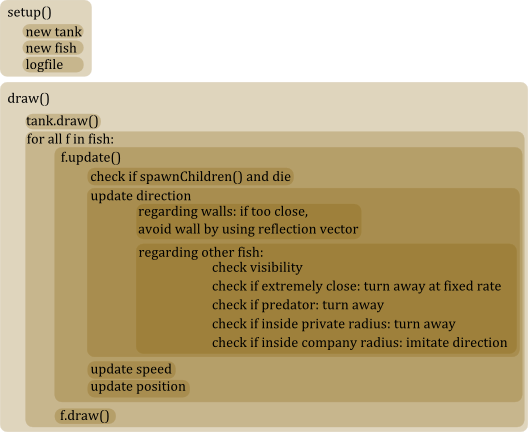
\includegraphics[width=\textwidth]{implementationsketch}
        \caption{Essential structure of the program}
        
\end{figure}

\subsection{Exporting the Values}
To be able to extract all important positions and values from the program I implemented several logging methods. The program produces a simple text-file, where the parameter values are noted as well as the positions of the fish (original coordinates plus coordinates scaled to fit the textile application), their id and their children. The tank class produces an image where the positions of the fish are noted pixelwise, the image shows their complete movement. I also export an SVG-file with a straight line connecting the end position of each fish with their children. This export can be done with additional text output directly within the SVG-file (the id of each fish above its "grave").

%TODO examples of the 3 log files
\begin{minipage}[t]{\textwidth}
\scriptsize
\begin{verbatim}
tank cx,cy,radius: 300.0 300.0 300.0
starter fish: 1
start dir: 0.0 -1.0
start pos: 300.0, 300.0
wall/neighbor 0.9/0.1
maxGenerations 6
maxChildren 2

spawnTime 6000ms
spawnAnglesDegree 135.0 -135.0
turnSpeed 0.011/ms
private radius / company radius 30.0 / 70.0

fish:
0 g:0 born 300.0 590.0 : 140 275 c: 
0 g:0 died 300.0 410.82532 : 140 192 c: 1 2 
1 g:1 died 331.64142 237.63405 : 155 111 c: 3 4 
2 g:1 died 264.66016 238.89192 : 124 111 c: 5 6 
3 g:2 died 375.58804 65.089584 : 175 30 c: 7 8 
...
\end{verbatim}
\captionof{figure}{The text-based log file consists of all important parameters as well as the coordinates of each fish, g: denotes the generation while c: denotes the ids of its descendents.}
\end{minipage}
\vspace{0.5cm}

\begin{minipage}[t]{0.46\textwidth}
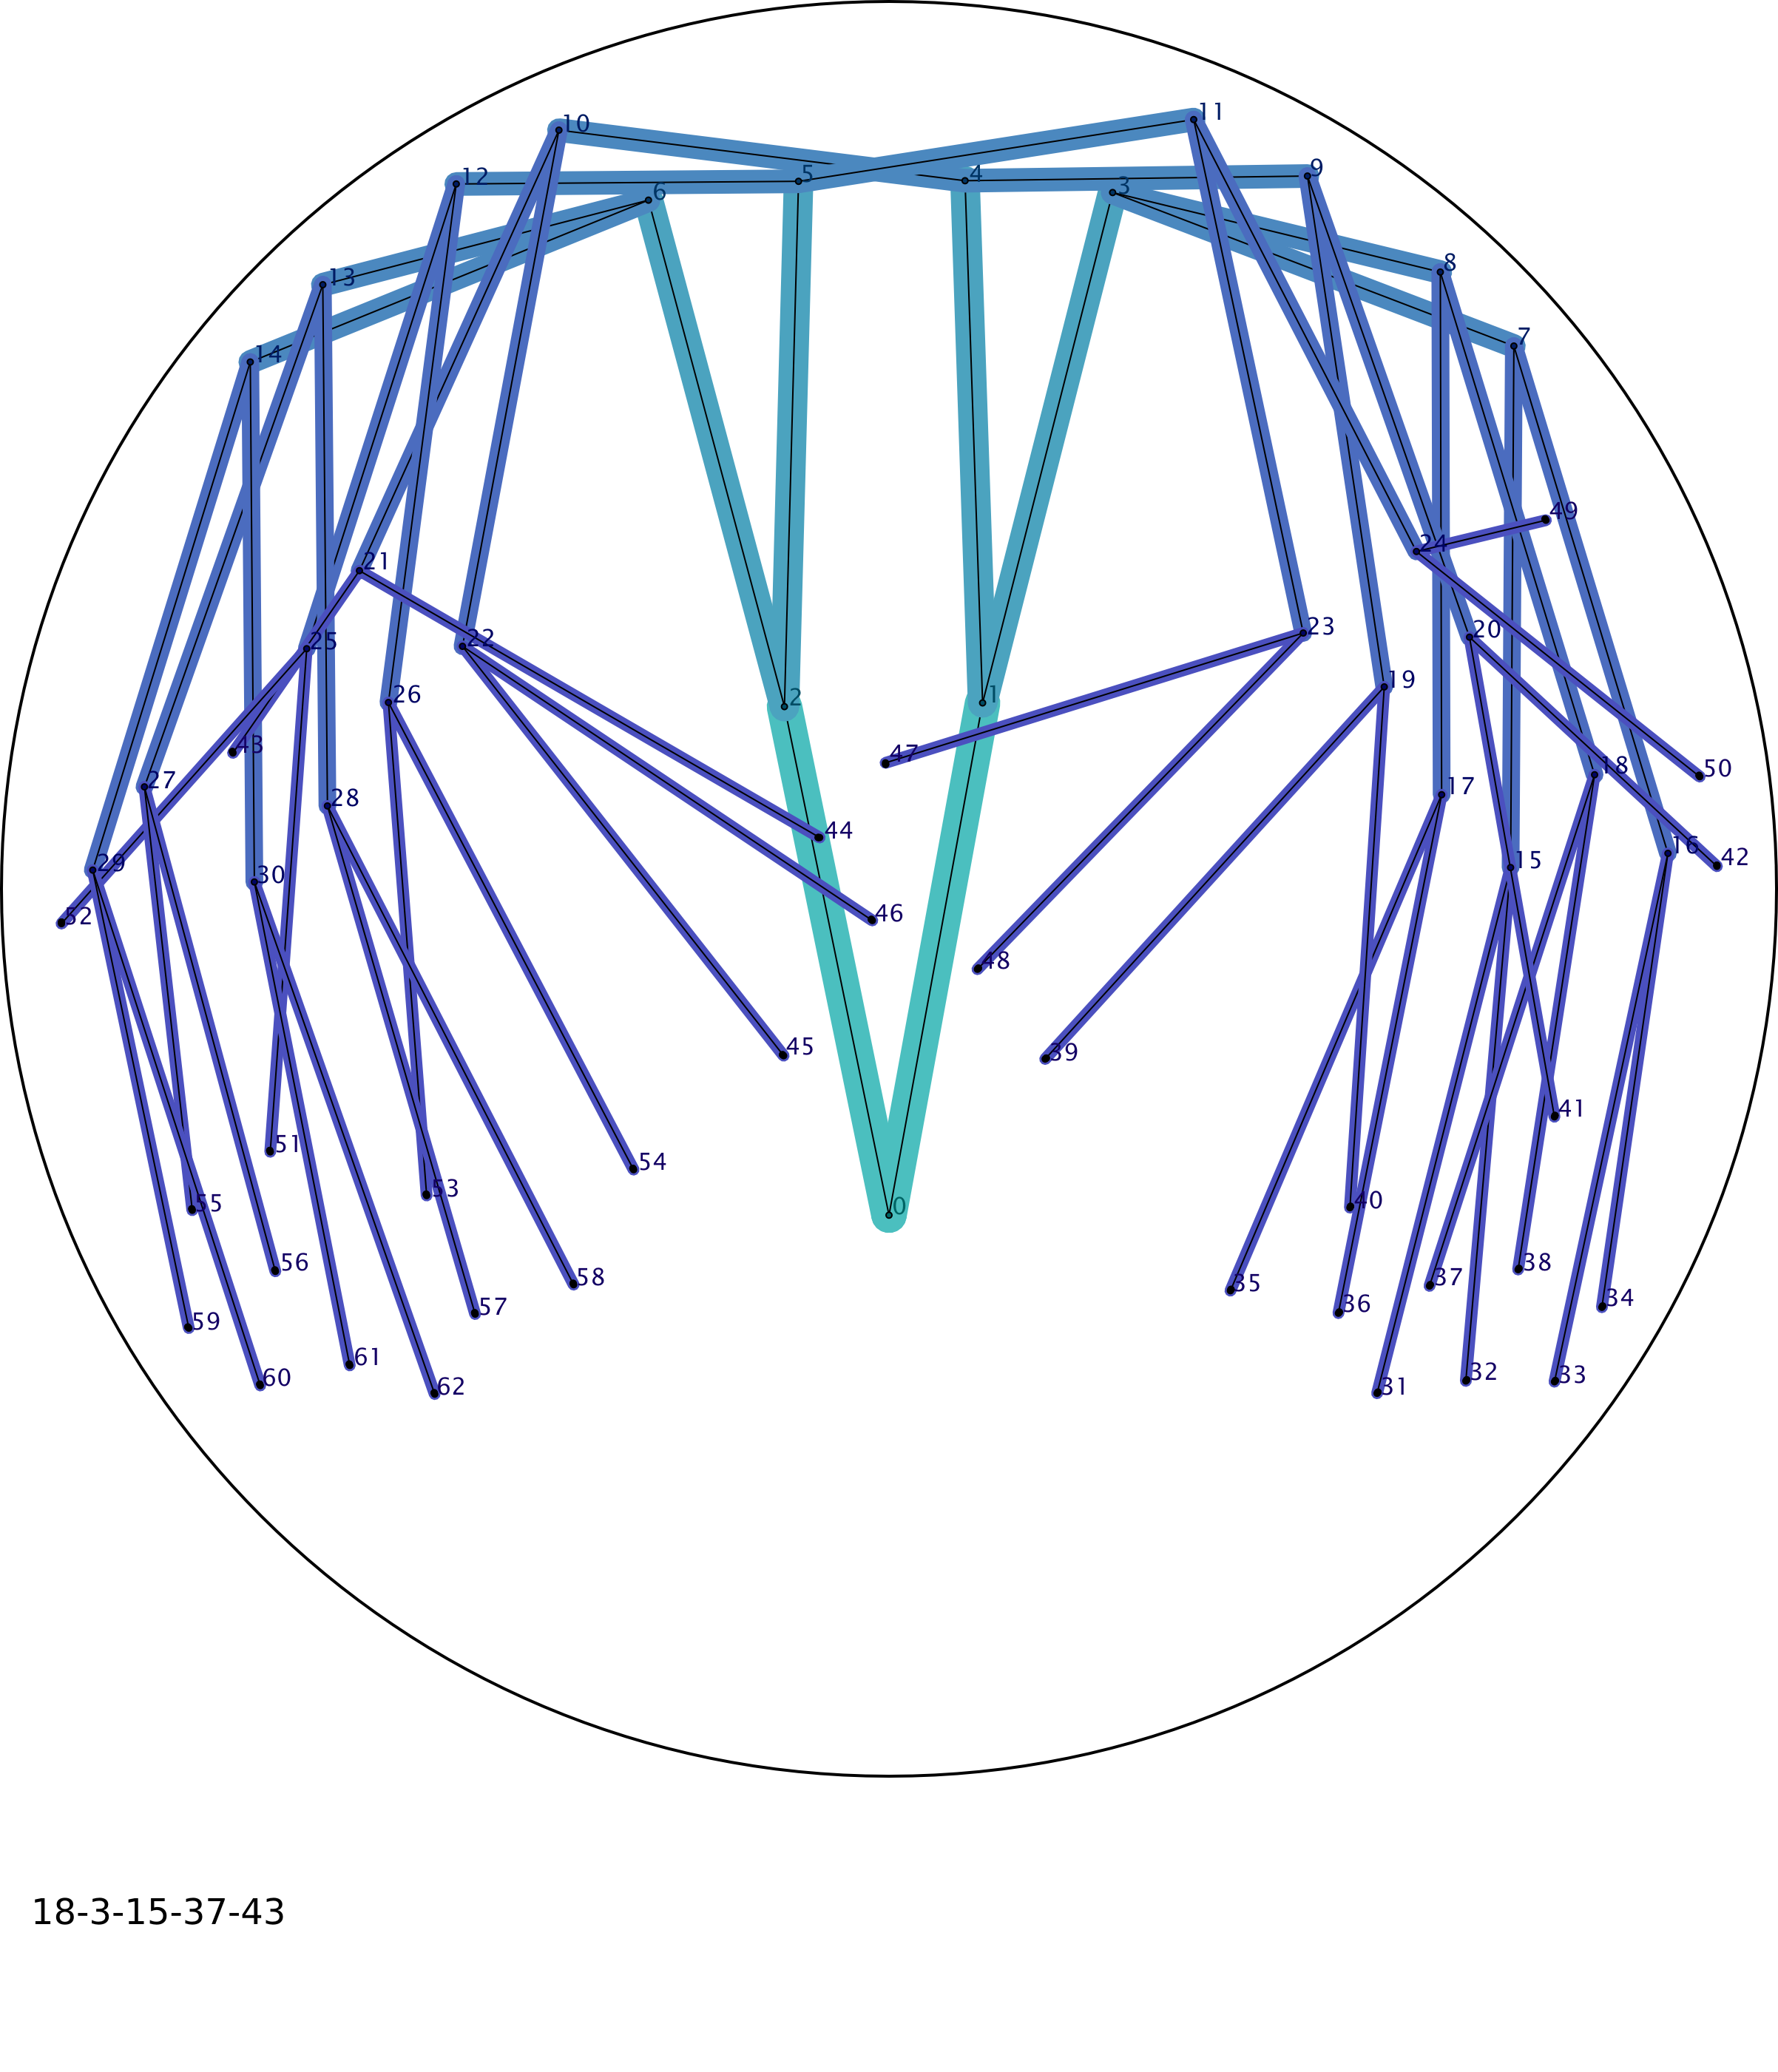
\includegraphics[width=\textwidth]{img_18-3-15-37-43}
\captionof{figure}{Connection lines between (dead) fish of 6 generations}
\end{minipage}
\hspace{0.5cm}
\begin{minipage}[t]{0.46\textwidth}
\raisebox{0.175\totalheight}{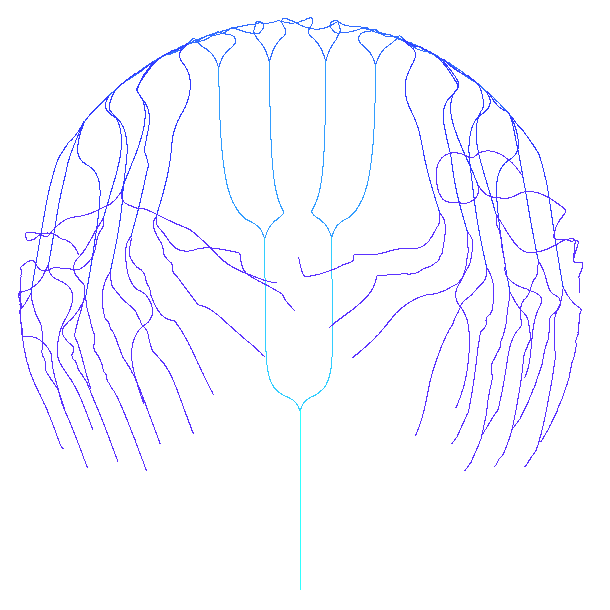
\includegraphics[width=\textwidth]{tank_default_trace_18-3-15-37-43_1}}
\captionof{figure}{Traces of the movement of the fish while living}
\end{minipage}
\vspace{0.5cm}

\subsection{Parameters and Variations}
There are several more, but some of the most important fish parameters and properties are:
\begin{description}
\item[privateRadius] If another fish is within this distance (in pixel) the current fish moves away from it.
\item[companyRadius] If another fish is within this distance (in pixel) the current fish imitates the other fish's movement (linear interpolation between current direction vector and target direction vector).
\item[interpolationSpeed (speed of turns)] This value is interpreted as the number of milliseconds which are needed to reach the target vector with linear interpolation. Since interpolation is mainly used when a fish changes its direction vector it can also be called speed of turns (in 1/milliseconds).
\item[timetoSpawn] This is the life span of one fish (in milliseconds), in the moment of dying it will generate two new fish.
\item[spawnAnglesDegree] This array contains the angles (in degrees) for the initial direction of each child (relative to the parent's direction).
\end{description}

When varying one parameter the others are set to a default value to cleanly separate the effects of the change.
The "baseline" setting with all parameters set to default is included in each of the variation series, the natural order of the parameter sizes detemines its placement within the series (ordered by increasing values). Table \ref{table:variation} shows the used integer values.

\begin{center}
\begin{tabular}{ l | c | c }
  \hline                       
  Parameters 		 & Default value 	& Variation \\
  \hline
  privateRadius 	 & 30 		& 20 30 40 50 \\
  companyRadius 	 & 70 		& 50 70 90 120 \\
  interpolationSpeed & 100 		& 50 100 150 200 250 350 \\
  timetoSpawn 		 & 6000 	& 3000 4000 5000 6000 8000 \\
  spawnAnglesDegree (+/-)  & 135 	& 0 20 45 90 135 180 \\
  \hline  
\end{tabular}
\captionof{table}{Used parameter values}
\label{table:variation}
\end{center}

The following images show the different outcomes for variations of the parameters. On the left you see the connections between related fish, on the right there are their movement traces (actual paths).

\subsubsection{Variations of "privateRadius"}

%20
\begin{minipage}[t]{\imgSize\textwidth}
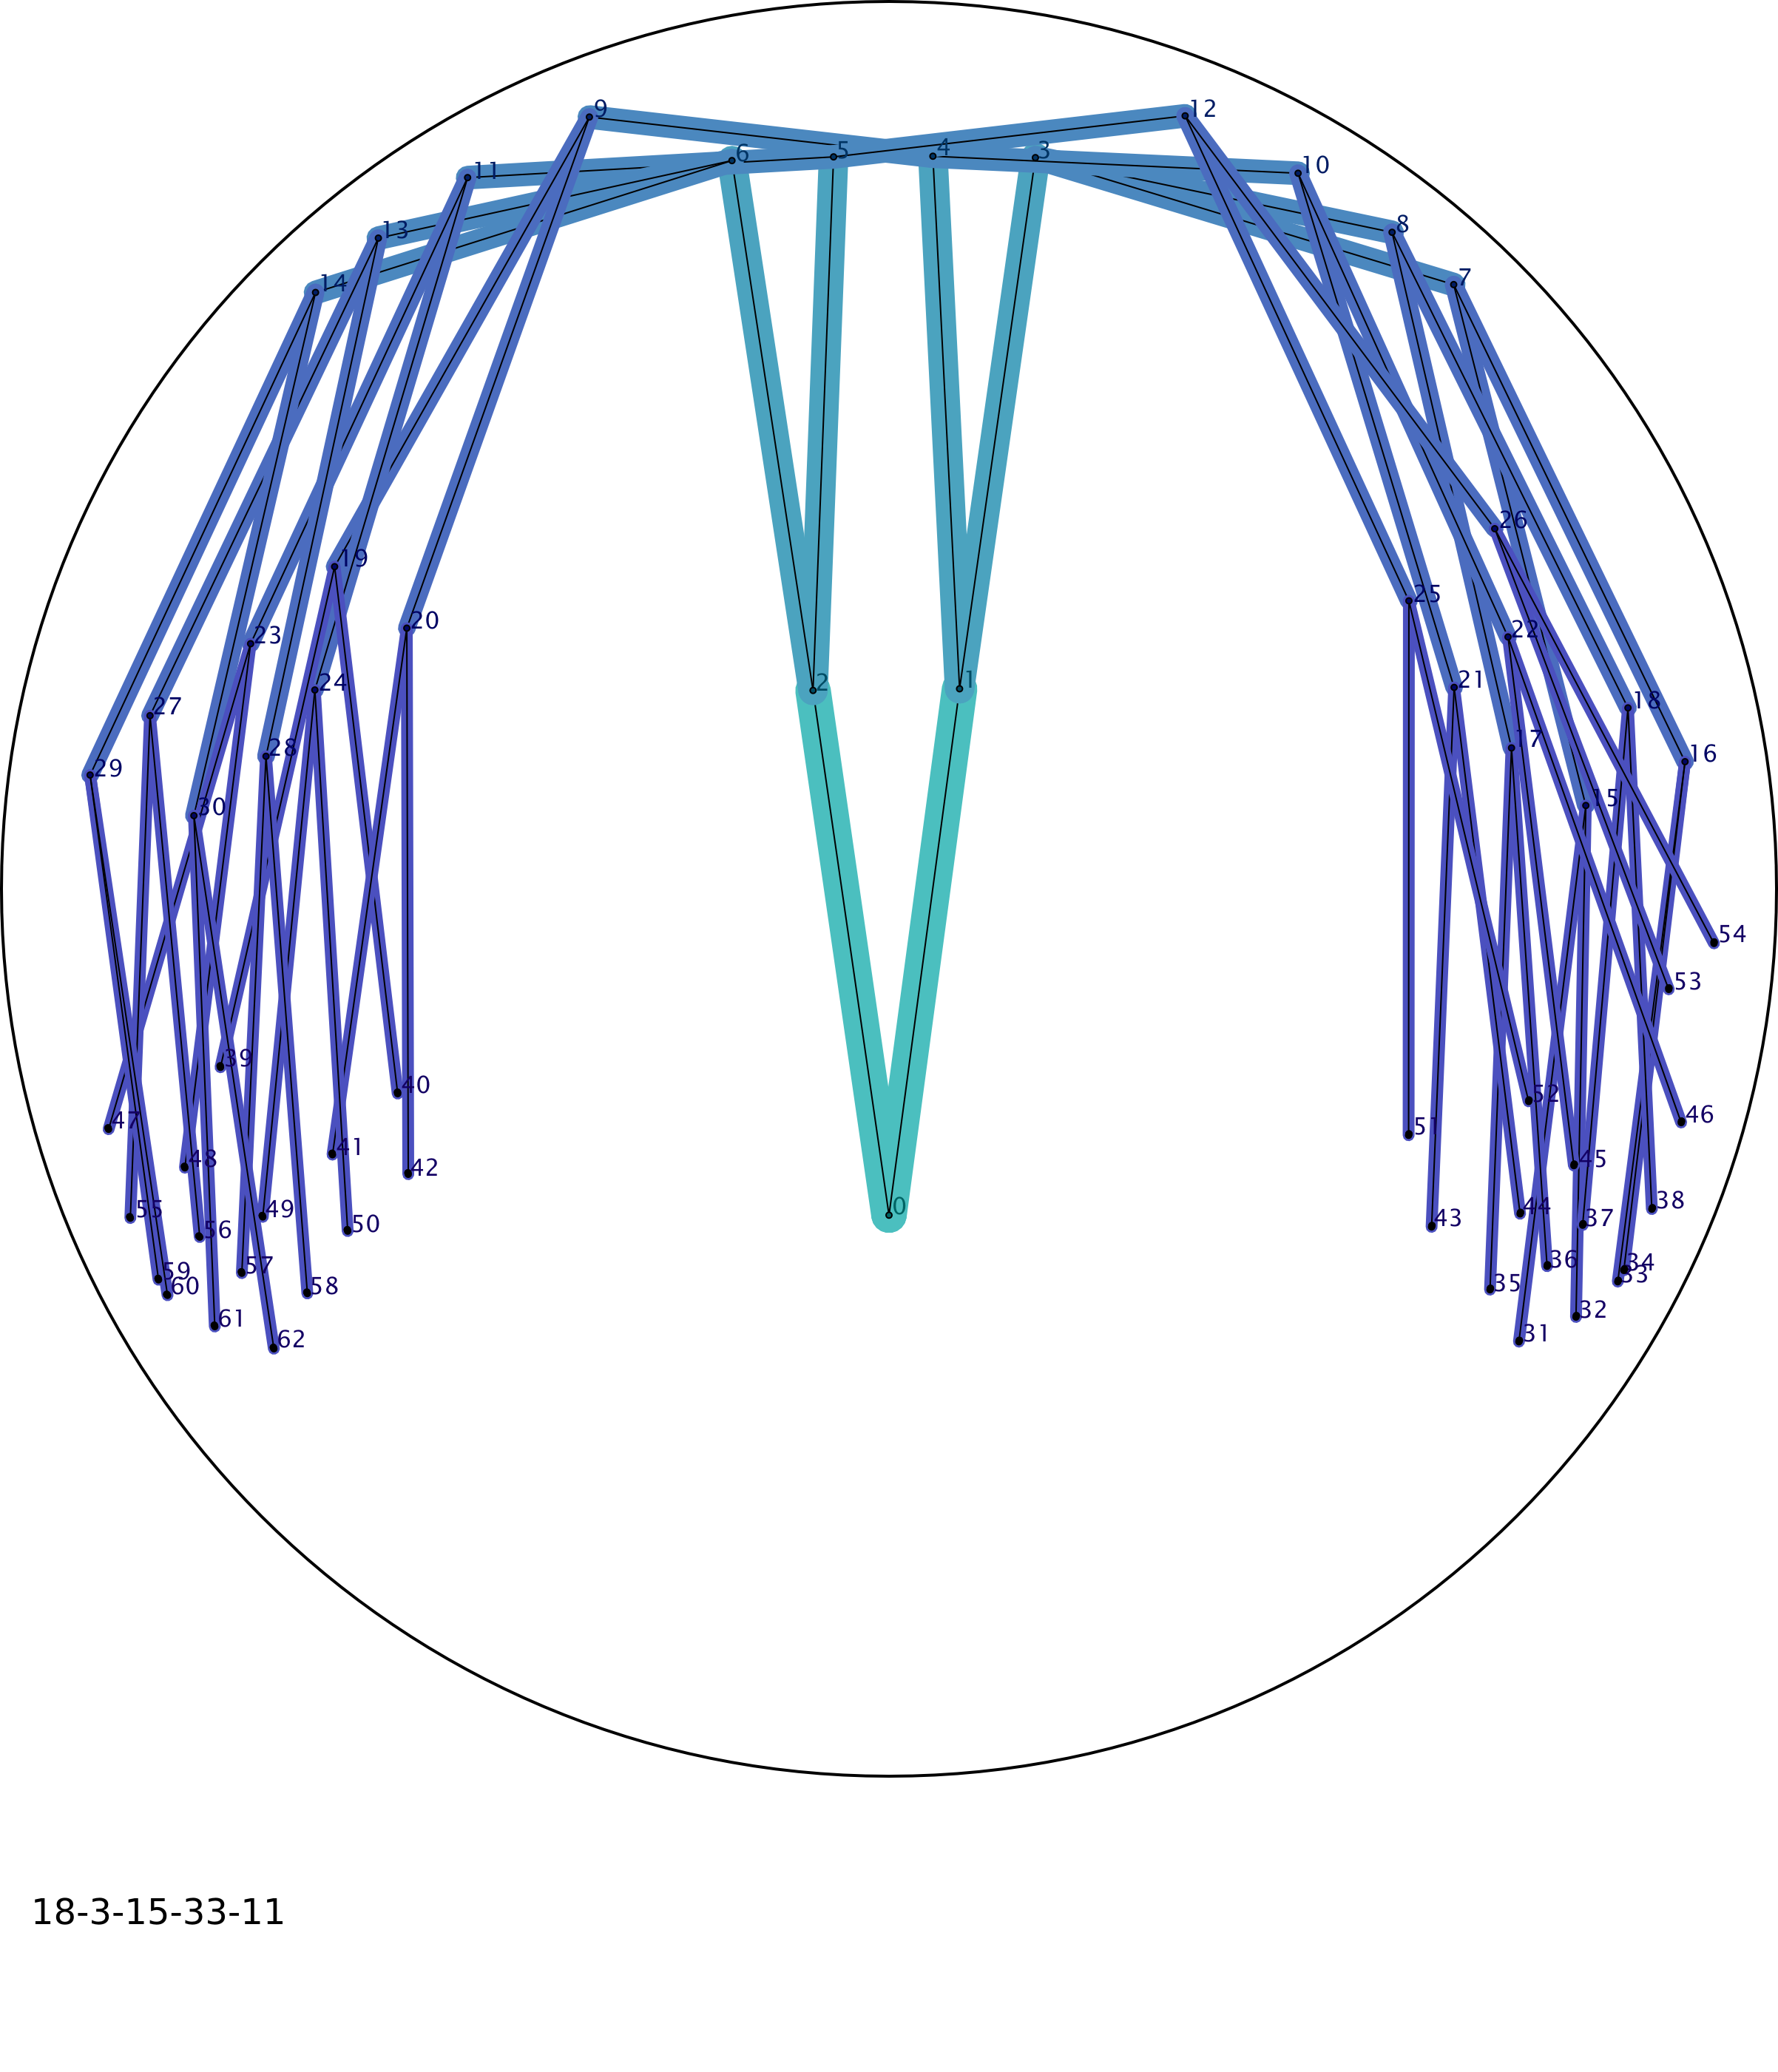
\includegraphics[width=\textwidth]{img_18-3-15-33-11}
\captionof{figure}{privateRadius = 20}
\end{minipage}
\hspace{0.5cm}
\begin{minipage}[t]{\imgSize\textwidth}
\raisebox{0.175\totalheight}{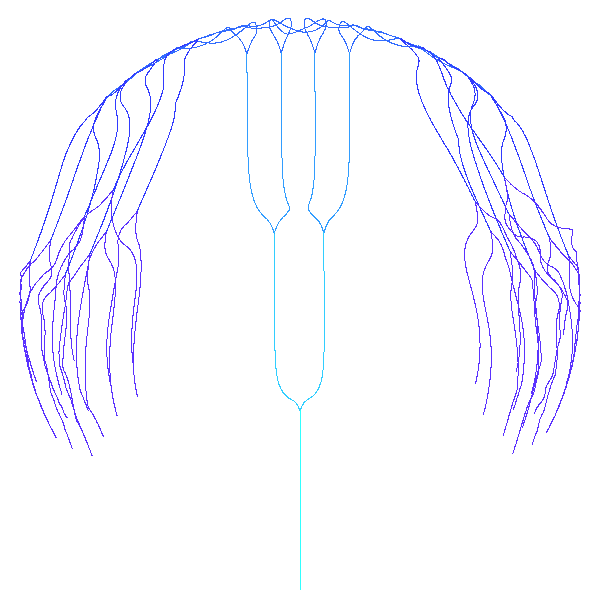
\includegraphics[width=\textwidth]{tank_privateRadius_trace_18-3-15-33-11_1}}
\captionof{figure}{privateRadius = 20}
\end{minipage}
\vspace{0.5cm}

%30
\begin{minipage}[t]{\imgSize\textwidth}
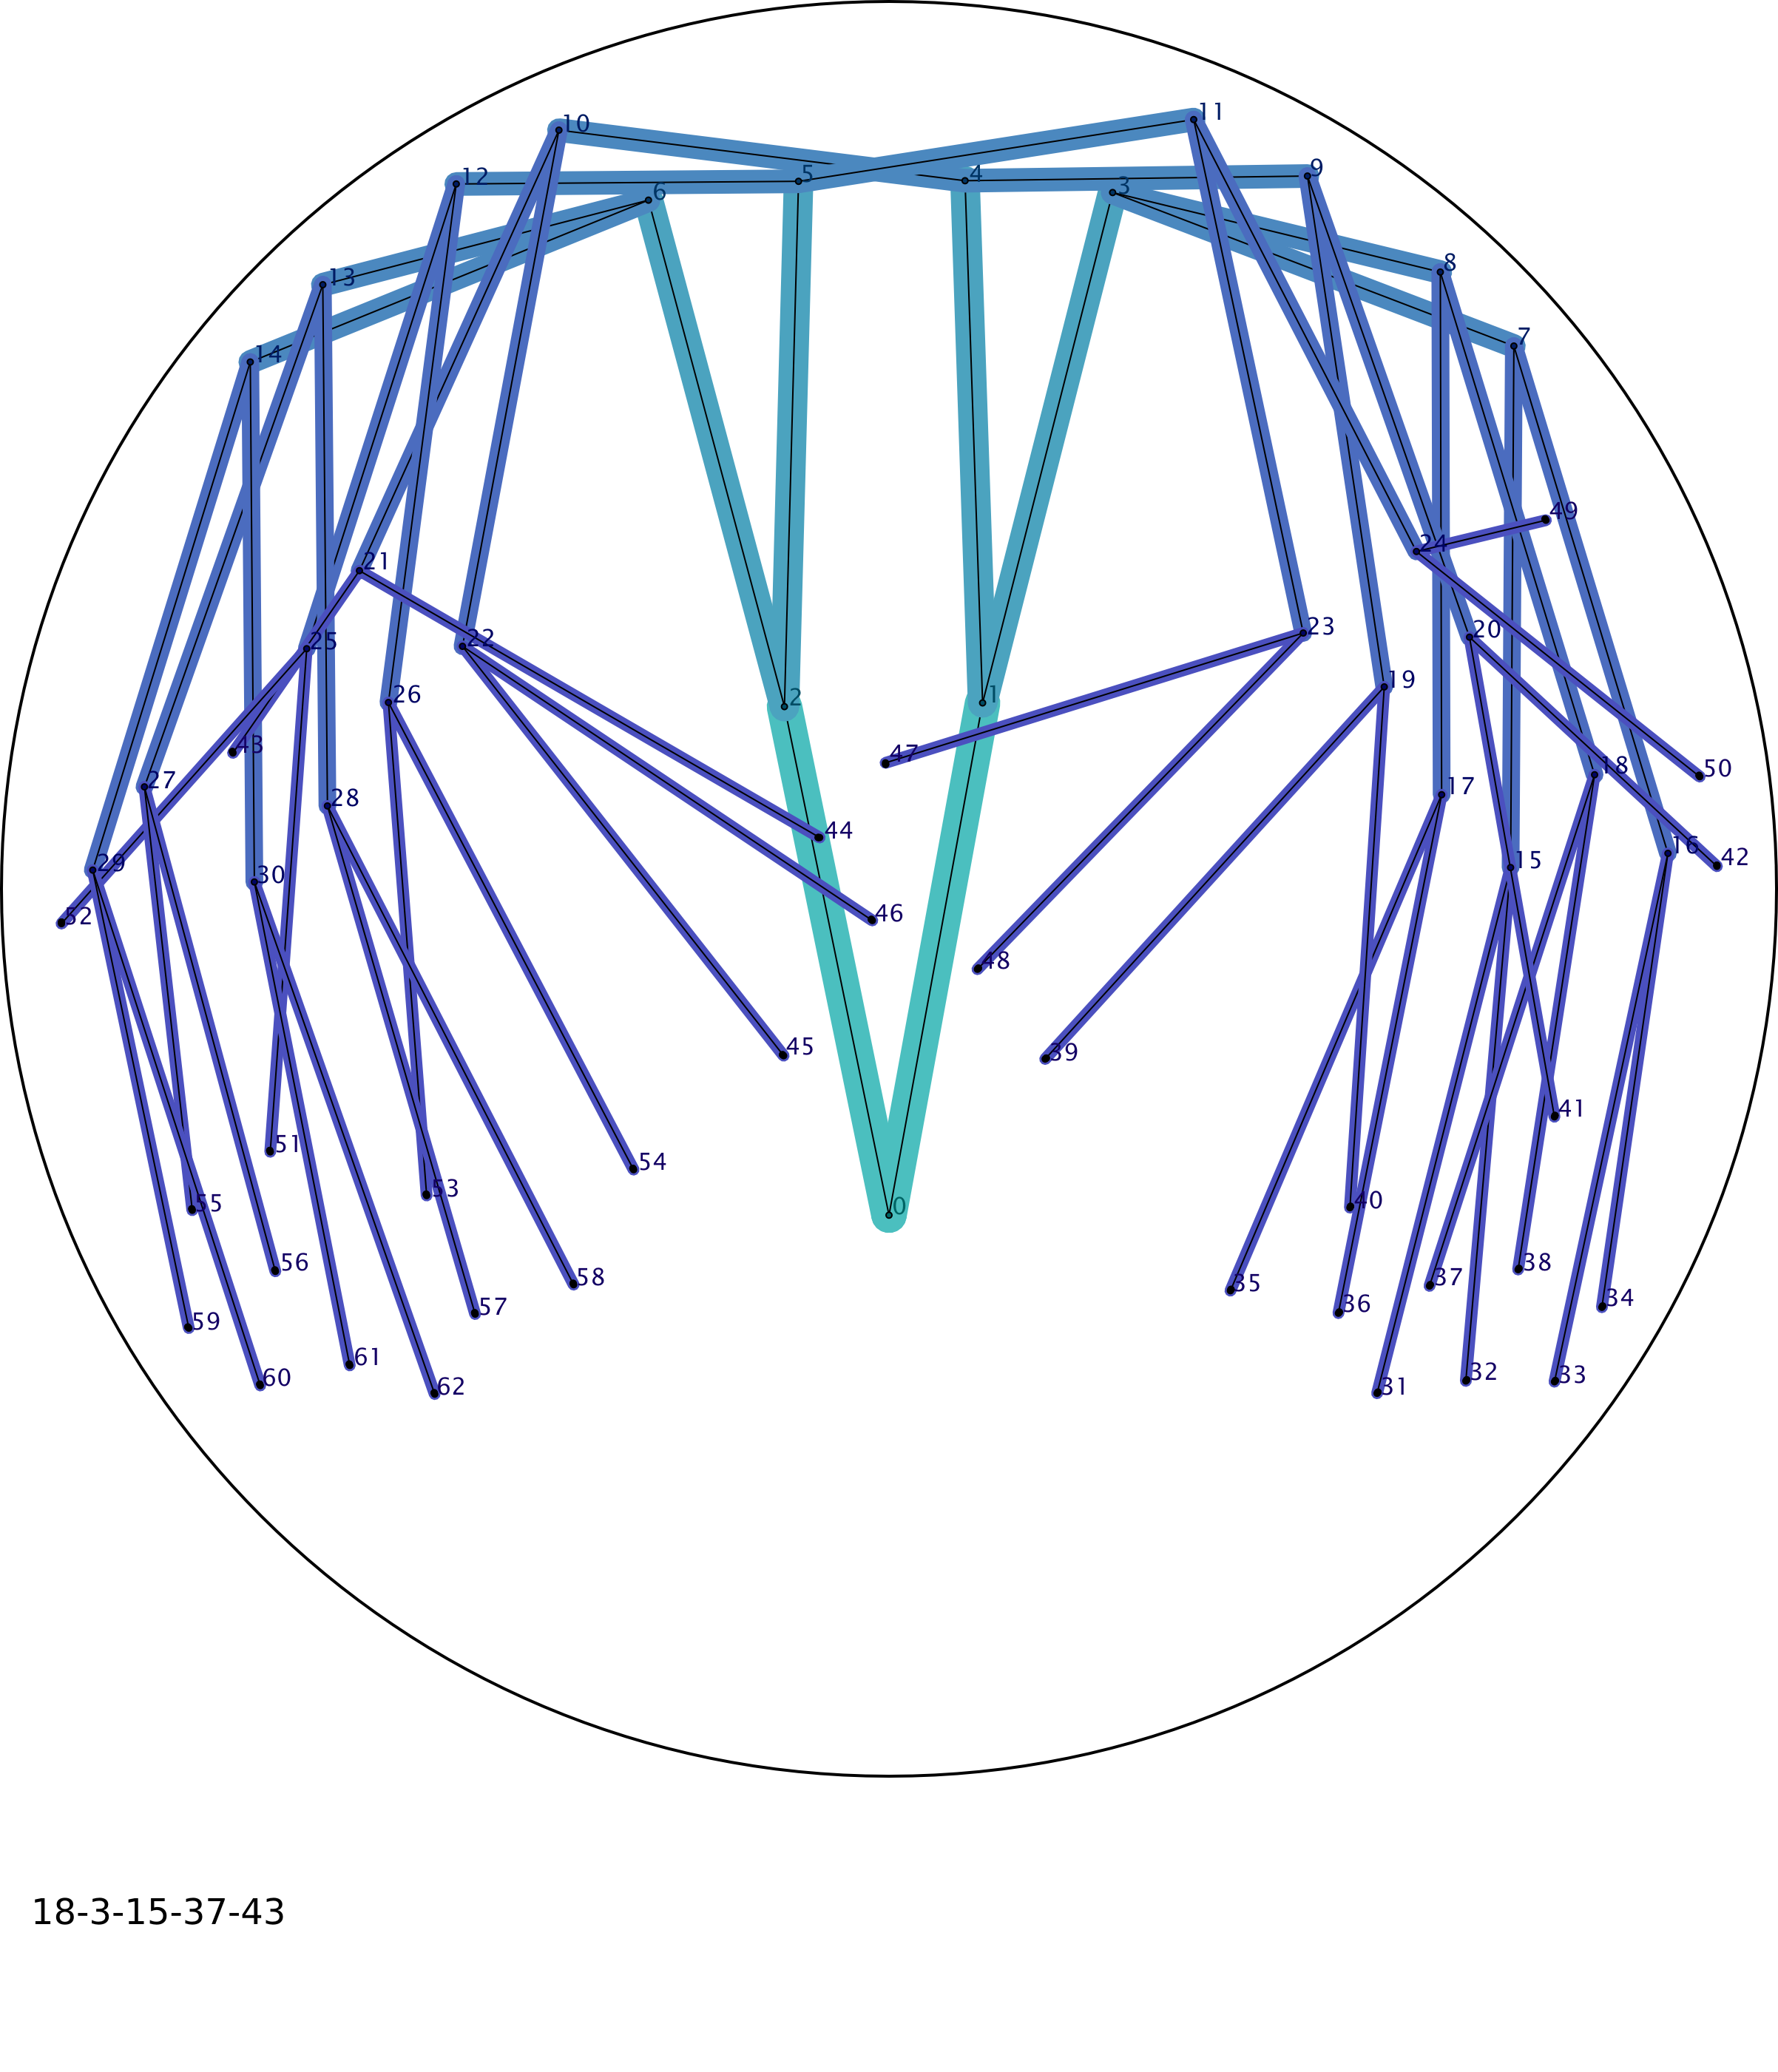
\includegraphics[width=\textwidth]{img_18-3-15-37-43}
\captionof{figure}{privateRadius = 30 (default)}
\end{minipage}
\hspace{0.5cm}
\begin{minipage}[t]{\imgSize\textwidth}
\raisebox{0.175\totalheight}{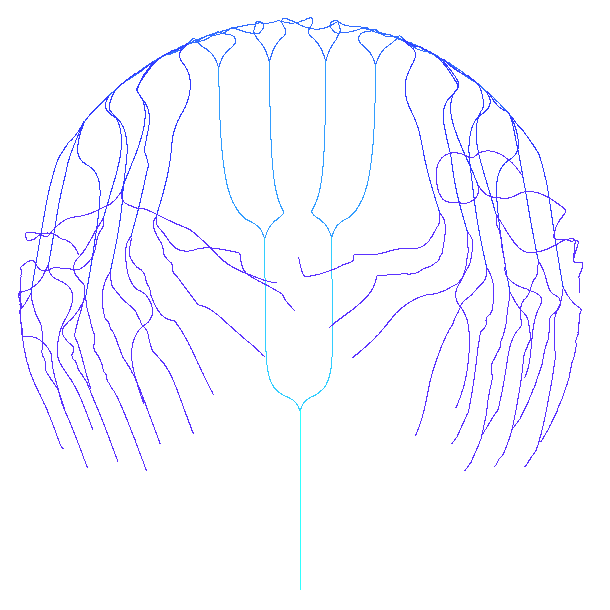
\includegraphics[width=\textwidth]{tank_default_trace_18-3-15-37-43_1}}
\captionof{figure}{privateRadius = 30 (default)}
\end{minipage}
\vspace{0.5cm}

%40
\begin{minipage}[t]{\imgSize\textwidth}
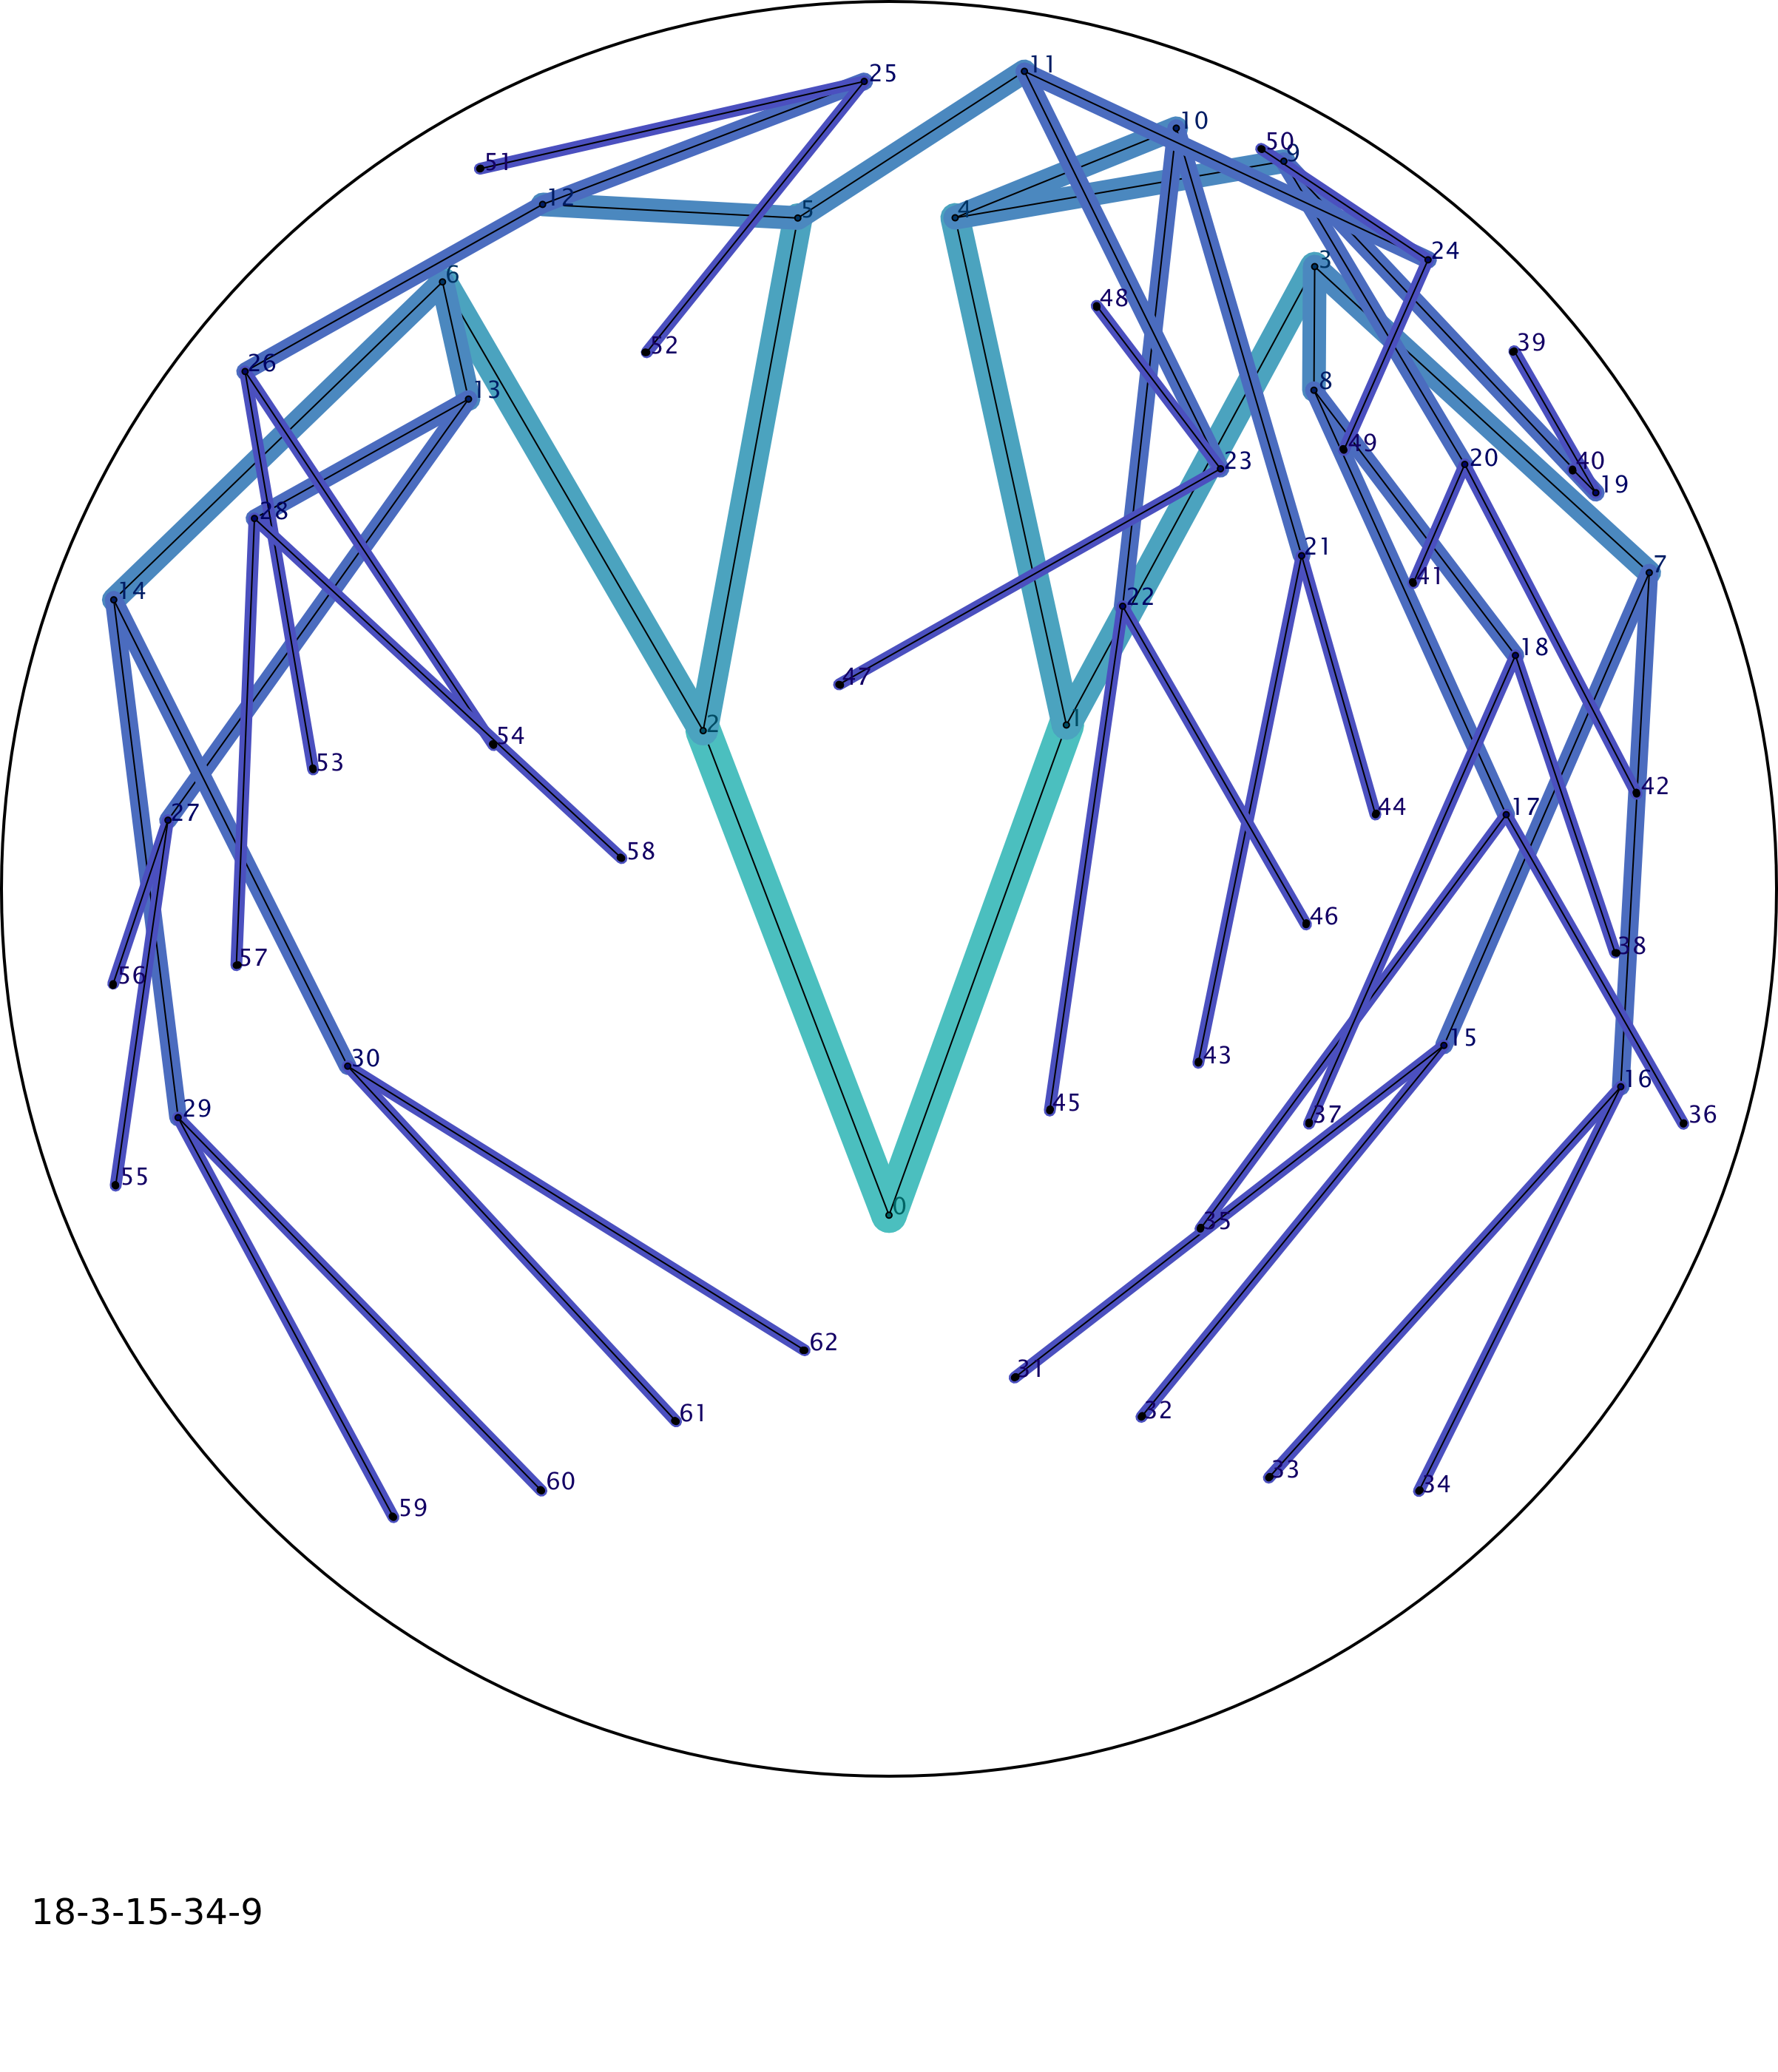
\includegraphics[width=\textwidth]{img_18-3-15-34-9}
\captionof{figure}{privateRadius = 40}
\end{minipage}
\hspace{0.5cm}
\begin{minipage}[t]{\imgSize\textwidth}
\raisebox{0.175\totalheight}{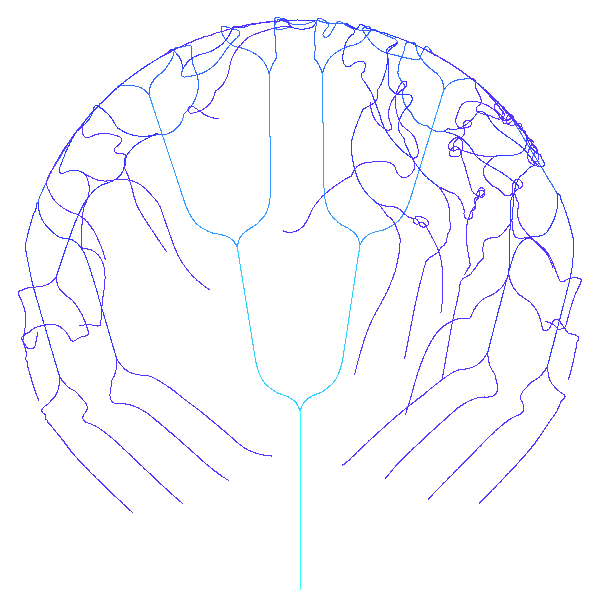
\includegraphics[width=\textwidth]{tank_privateRadius_trace_18-3-15-34-9_1}}
\captionof{figure}{privateRadius = 40}
\end{minipage}
\vspace{0.5cm}

%50
\begin{minipage}[t]{\imgSize\textwidth}
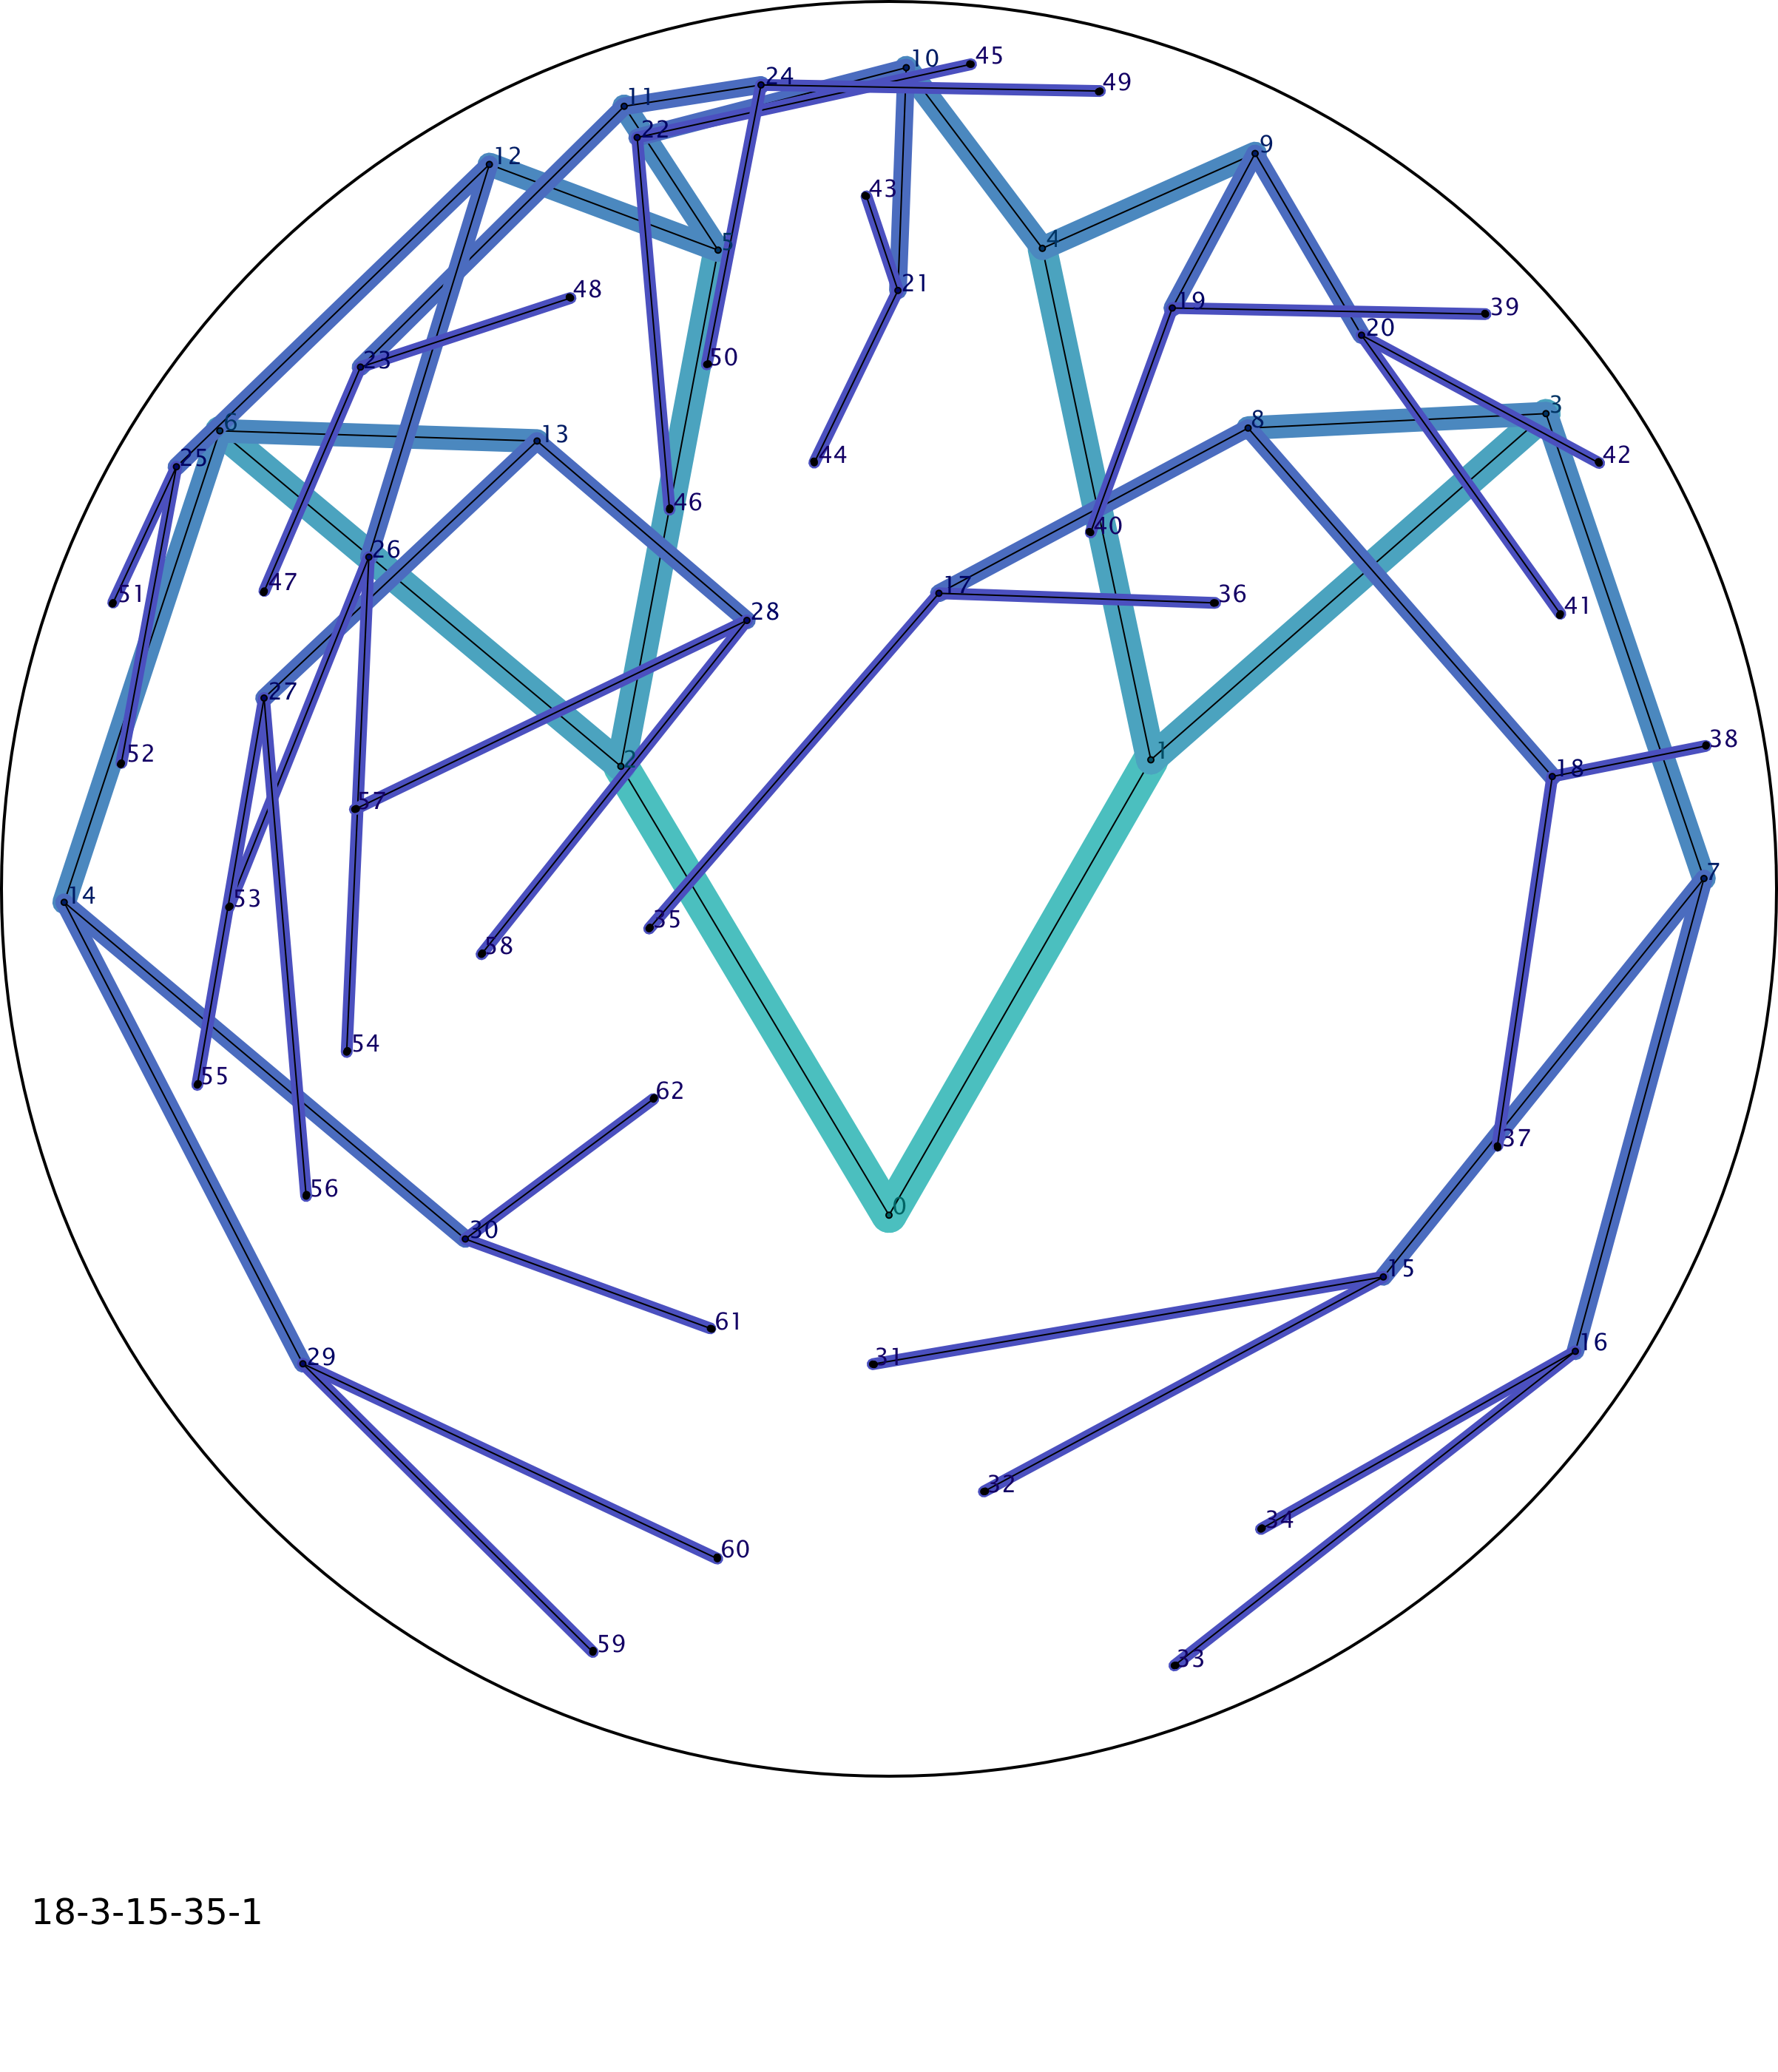
\includegraphics[width=\textwidth]{img_18-3-15-35-1}
\captionof{figure}{privateRadius = 50}
\end{minipage}
\hspace{0.5cm}
\begin{minipage}[t]{\imgSize\textwidth}
\raisebox{0.175\totalheight}{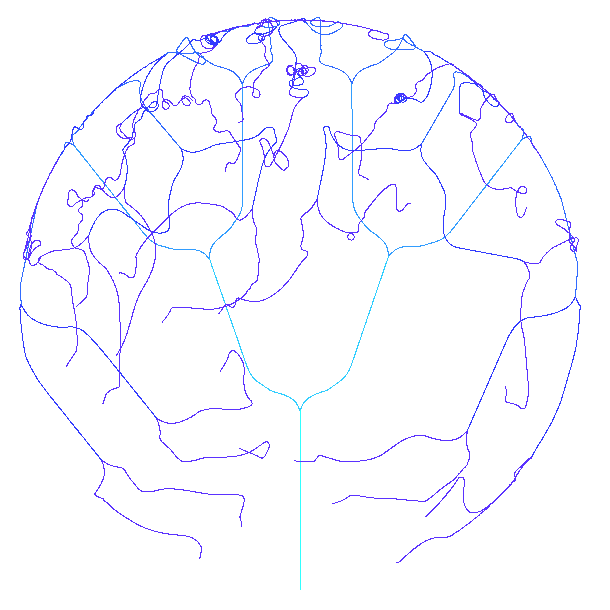
\includegraphics[width=\textwidth]{tank_privateRadius_trace_18-3-15-35-1_1}}
\captionof{figure}{privateRadius = 50}
\end{minipage}
\vspace{0.5cm}

\newpage
\subsubsection{Variations of "companyRadius"}

%50
\begin{minipage}[t]{\imgSize\textwidth}
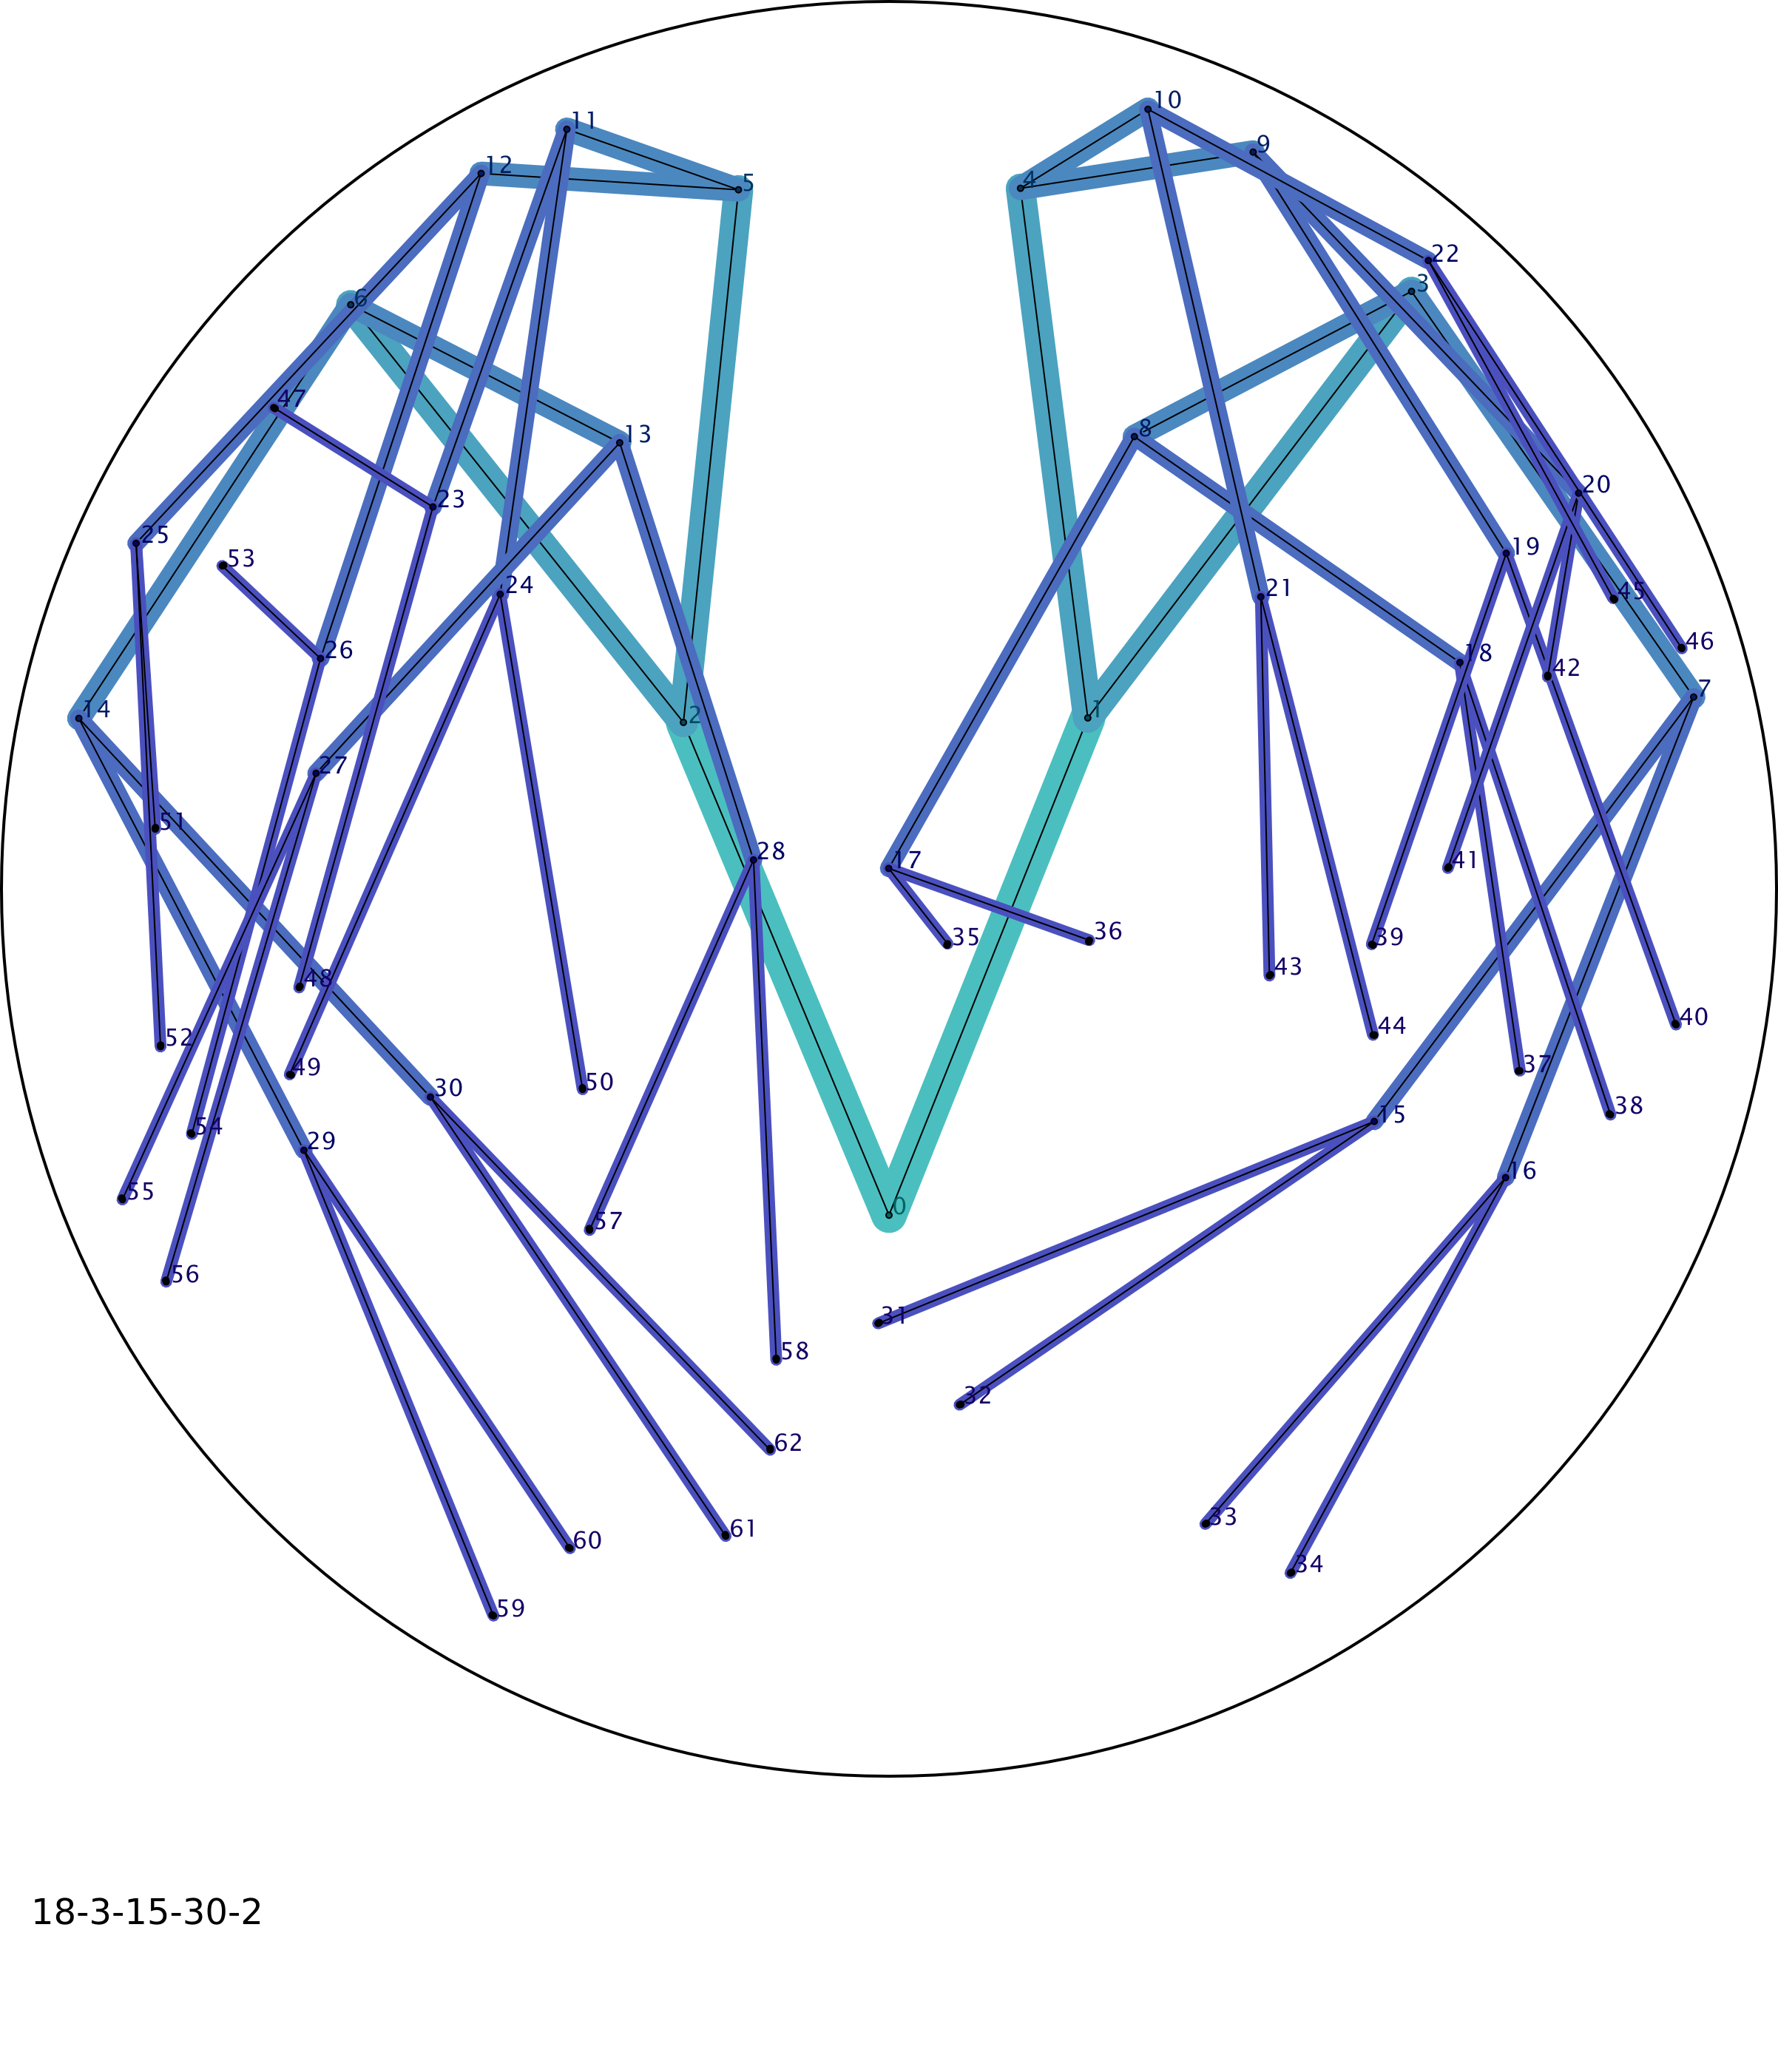
\includegraphics[width=\textwidth]{img_18-3-15-30-2}
\captionof{figure}{companyRadius = 50}
\end{minipage}
\hspace{0.5cm}
\begin{minipage}[t]{\imgSize\textwidth}
\raisebox{0.175\totalheight}{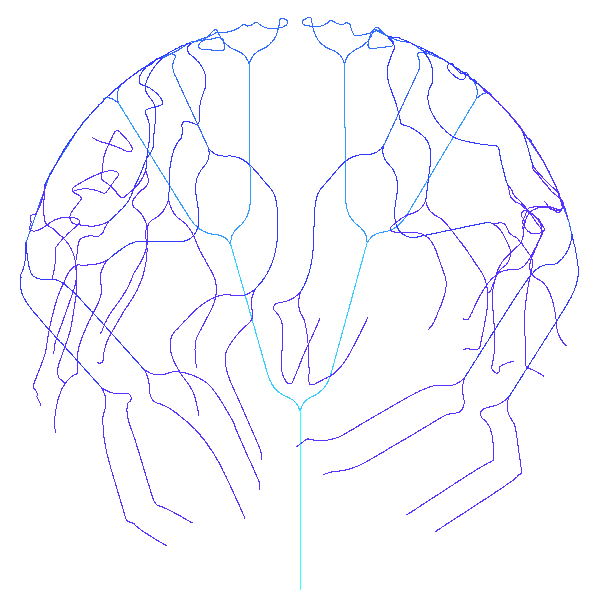
\includegraphics[width=\textwidth]{tank_companyRadius_trace_18-3-15-30-2_1}}
\captionof{figure}{companyRadius = 50}
\end{minipage}
\vspace{0.5cm}

%70
\begin{minipage}[t]{\imgSize\textwidth}
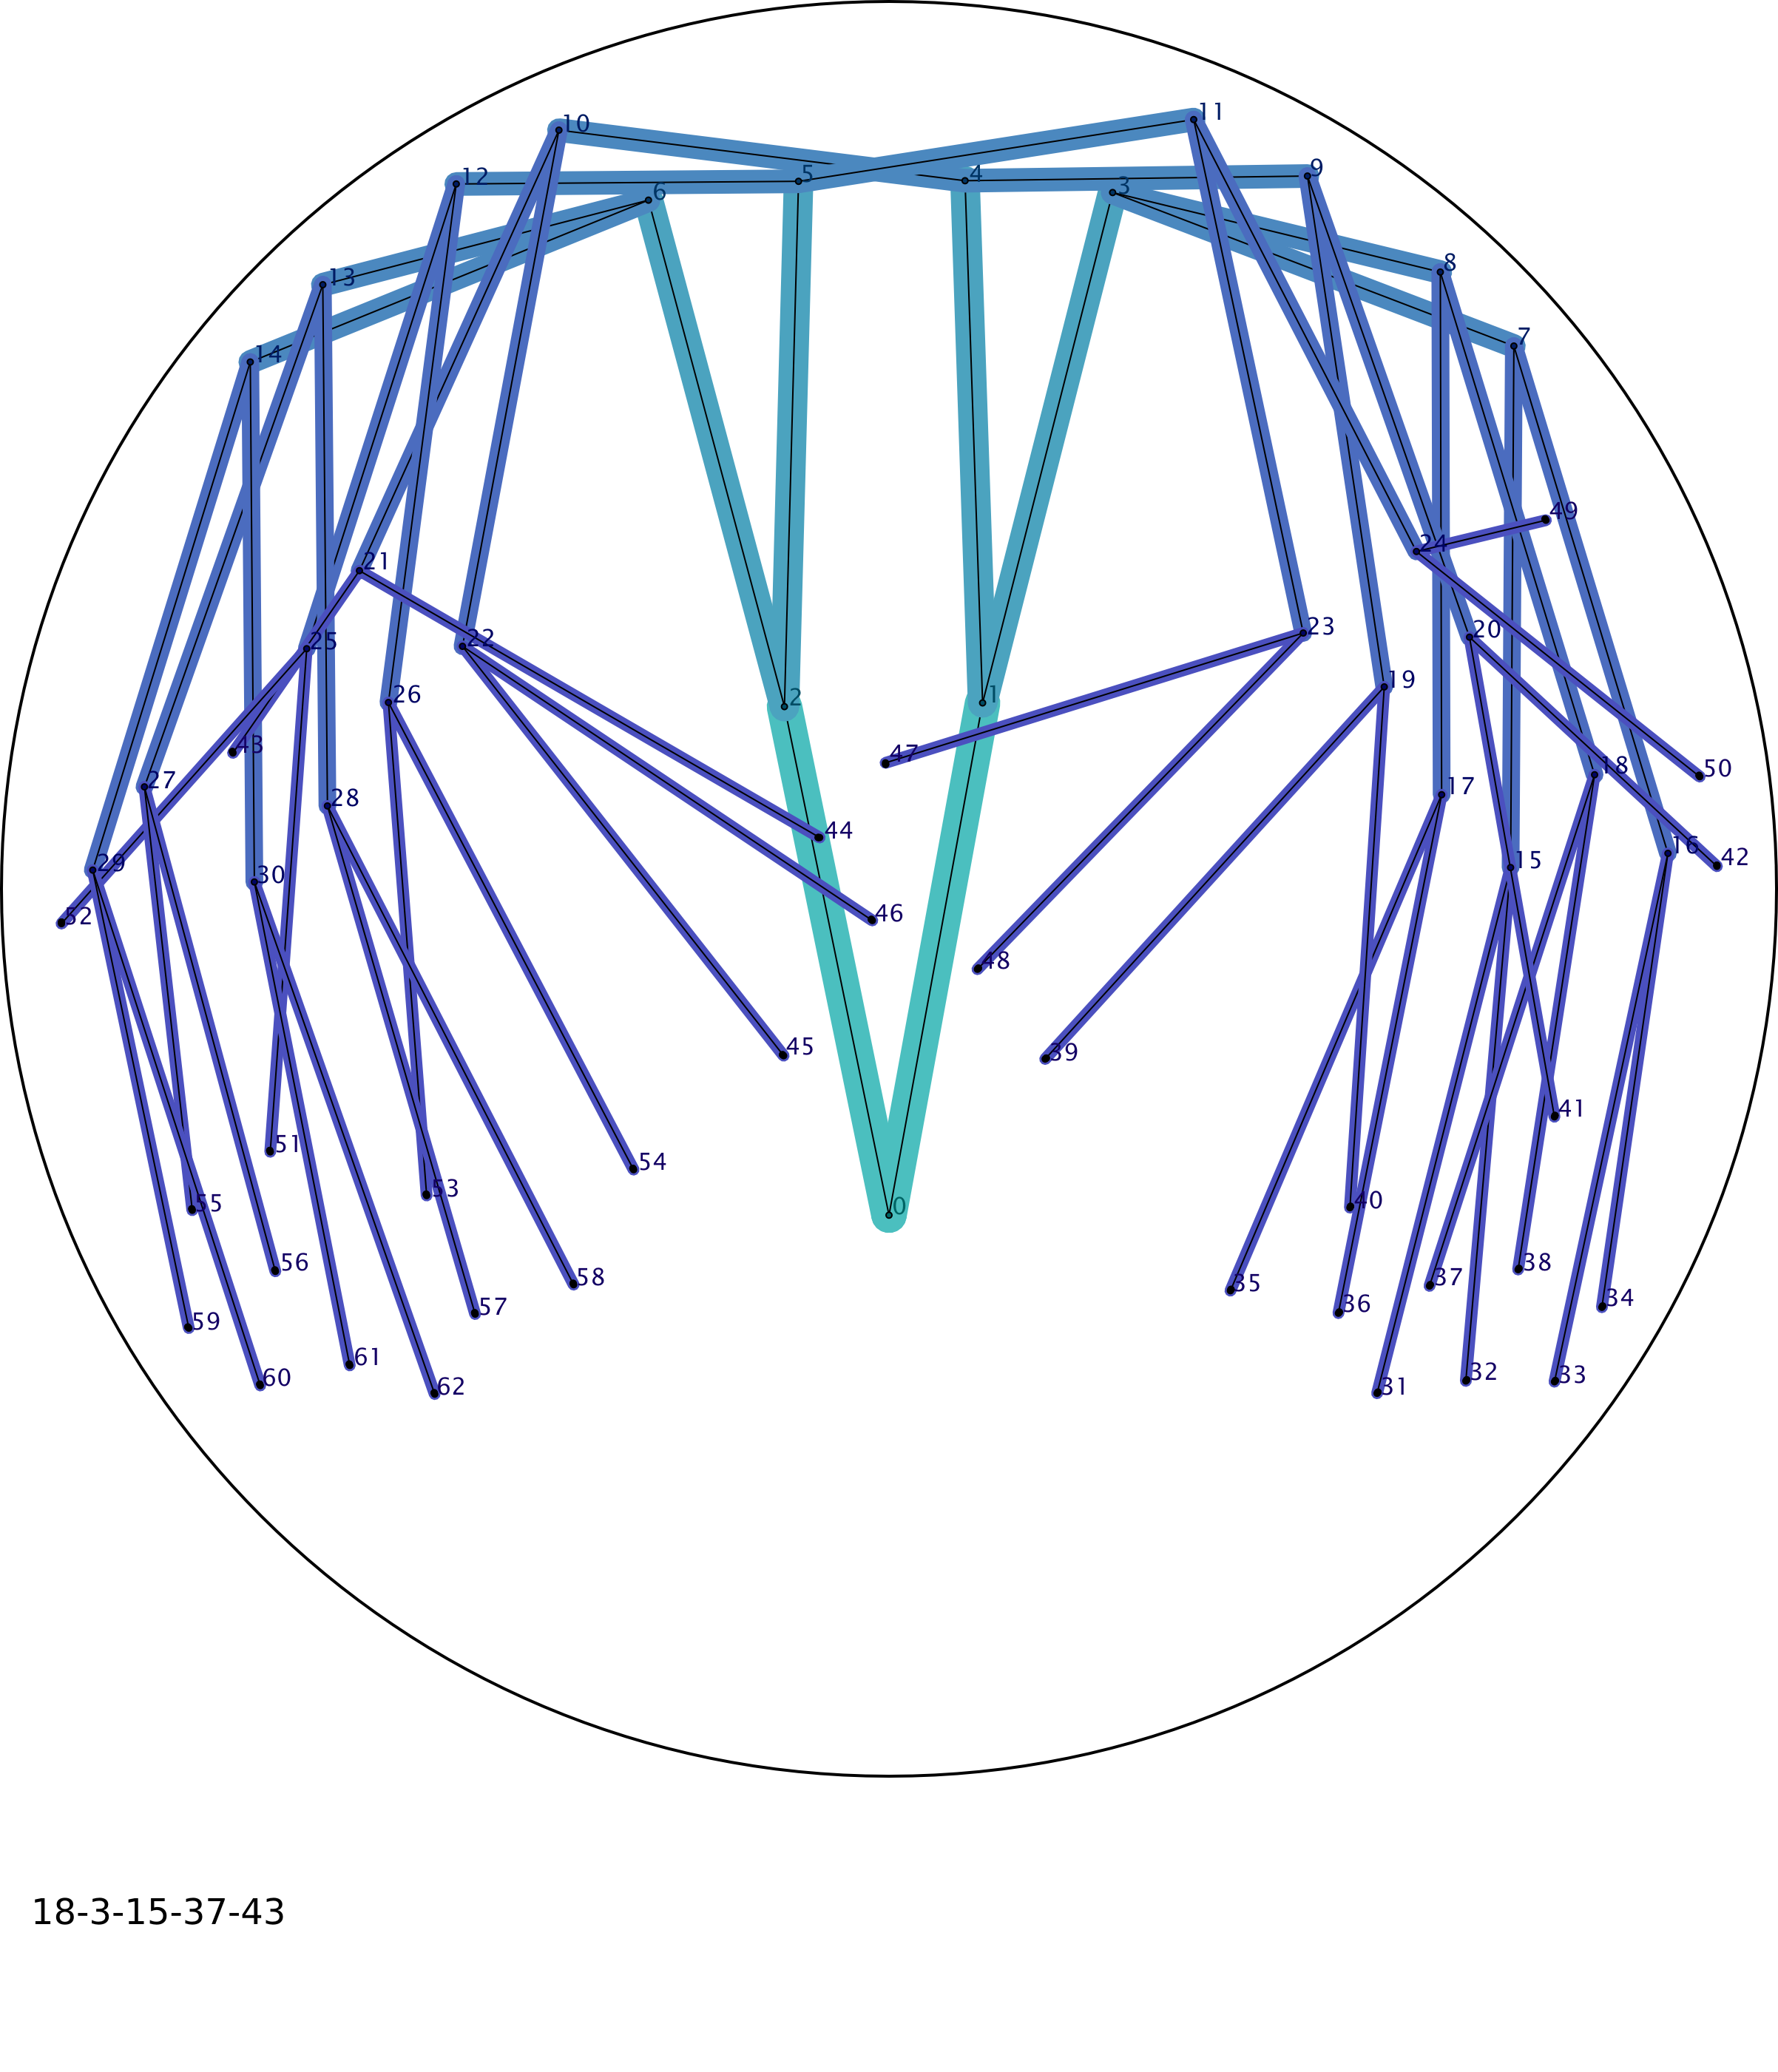
\includegraphics[width=\textwidth]{img_18-3-15-37-43}
\captionof{figure}{companyRadius = 70 (default)}
\end{minipage}
\hspace{0.5cm}
\begin{minipage}[t]{\imgSize\textwidth}
\raisebox{0.175\totalheight}{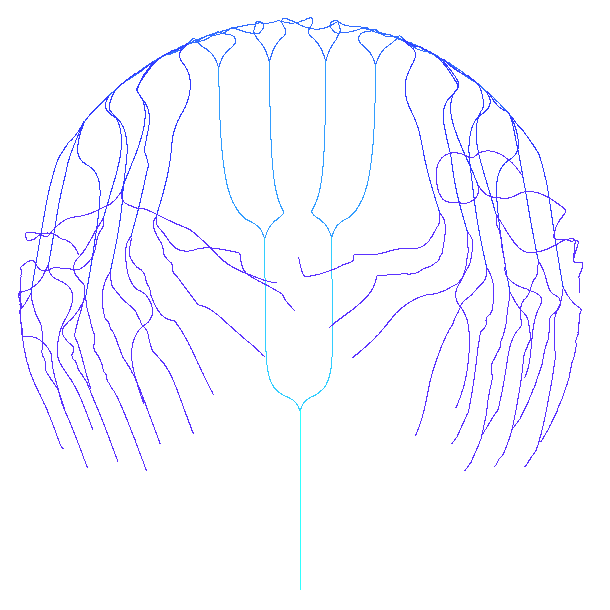
\includegraphics[width=\textwidth]{tank_default_trace_18-3-15-37-43_1}}
\captionof{figure}{companyRadius = 70 (default)}
\end{minipage}
\vspace{0.5cm}

%90
\begin{minipage}[t]{\imgSize\textwidth}
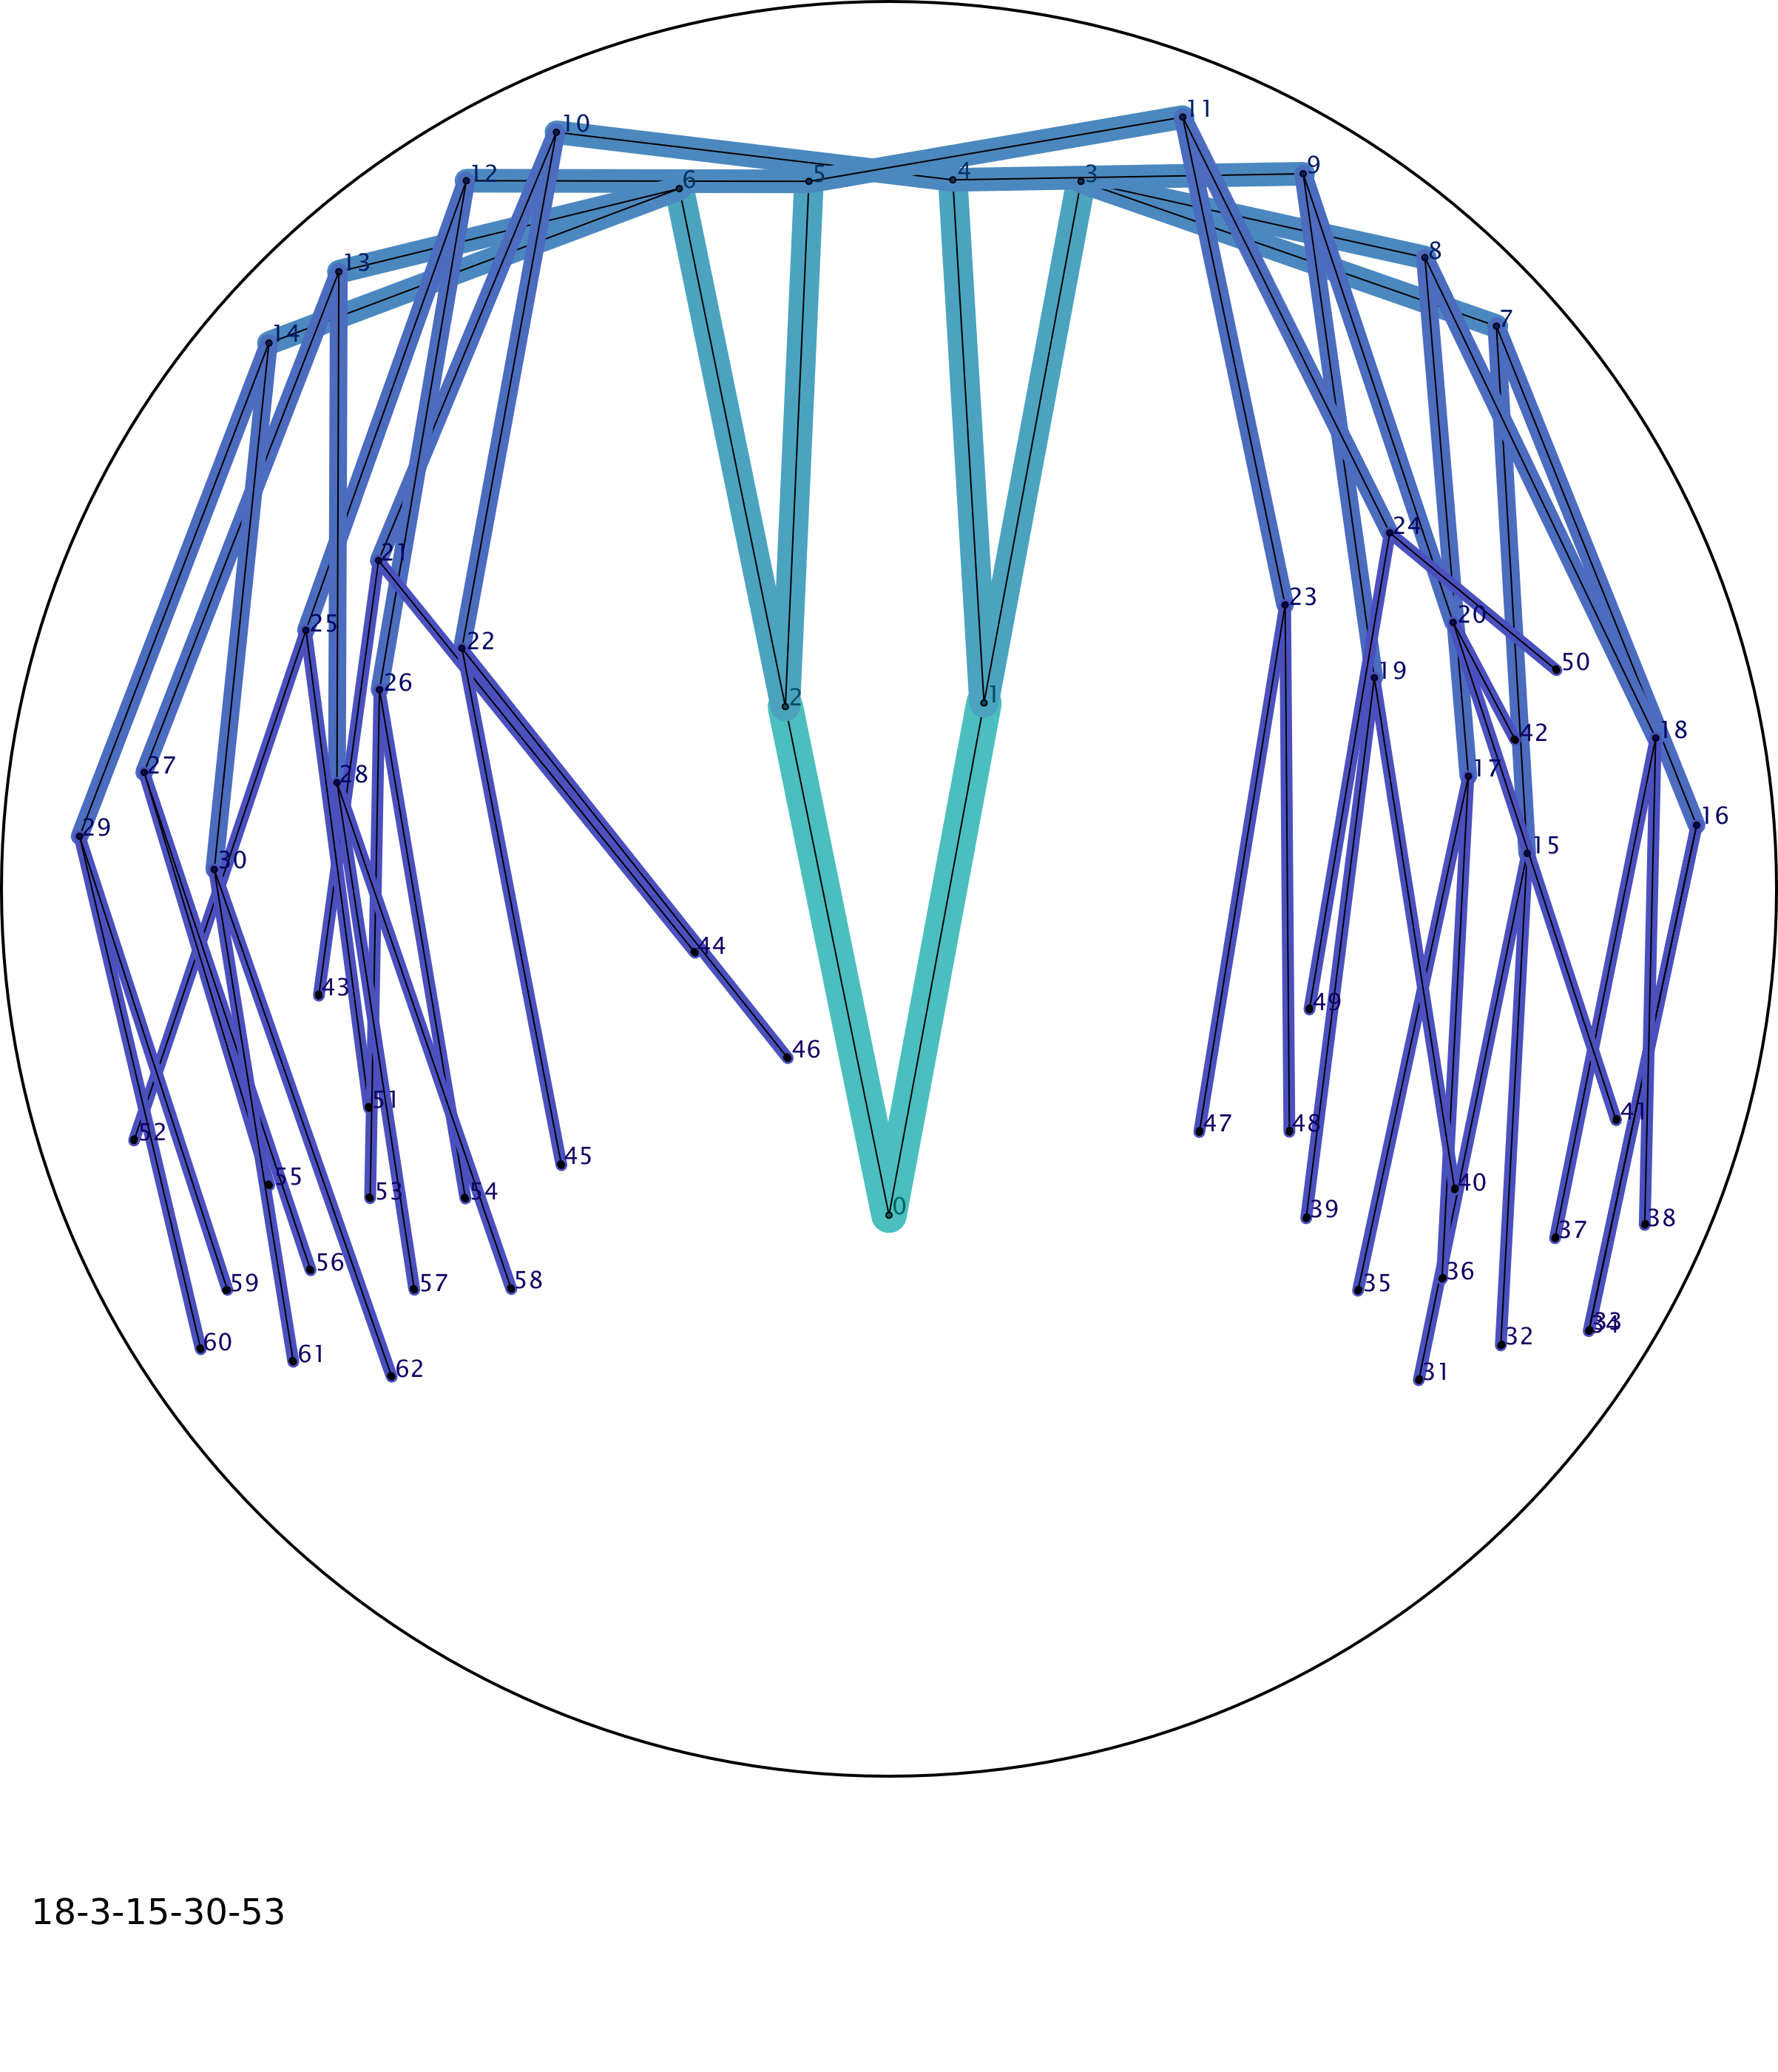
\includegraphics[width=\textwidth]{img_18-3-15-30-53}
\captionof{figure}{companyRadius = 90}
\end{minipage}
\hspace{0.5cm}
\begin{minipage}[t]{\imgSize\textwidth}
\raisebox{0.175\totalheight}{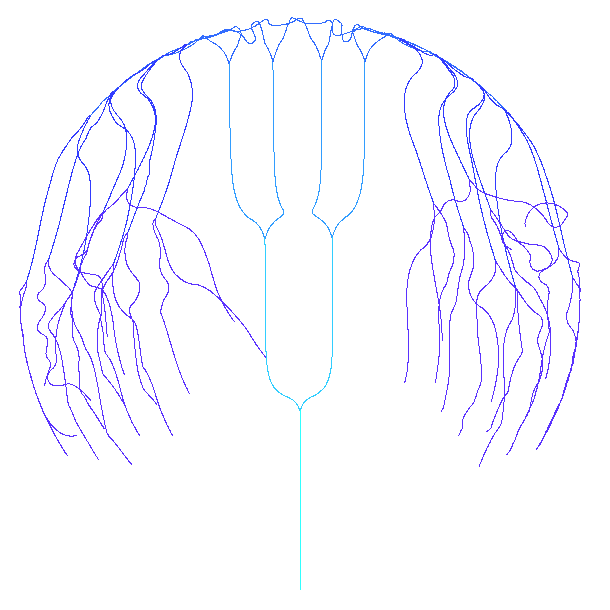
\includegraphics[width=\textwidth]{tank_companyRadius_trace_18-3-15-30-53_1}}
\captionof{figure}{companyRadius = 90}
\end{minipage}
\vspace{0.5cm}

%120
\begin{minipage}[t]{\imgSize\textwidth}
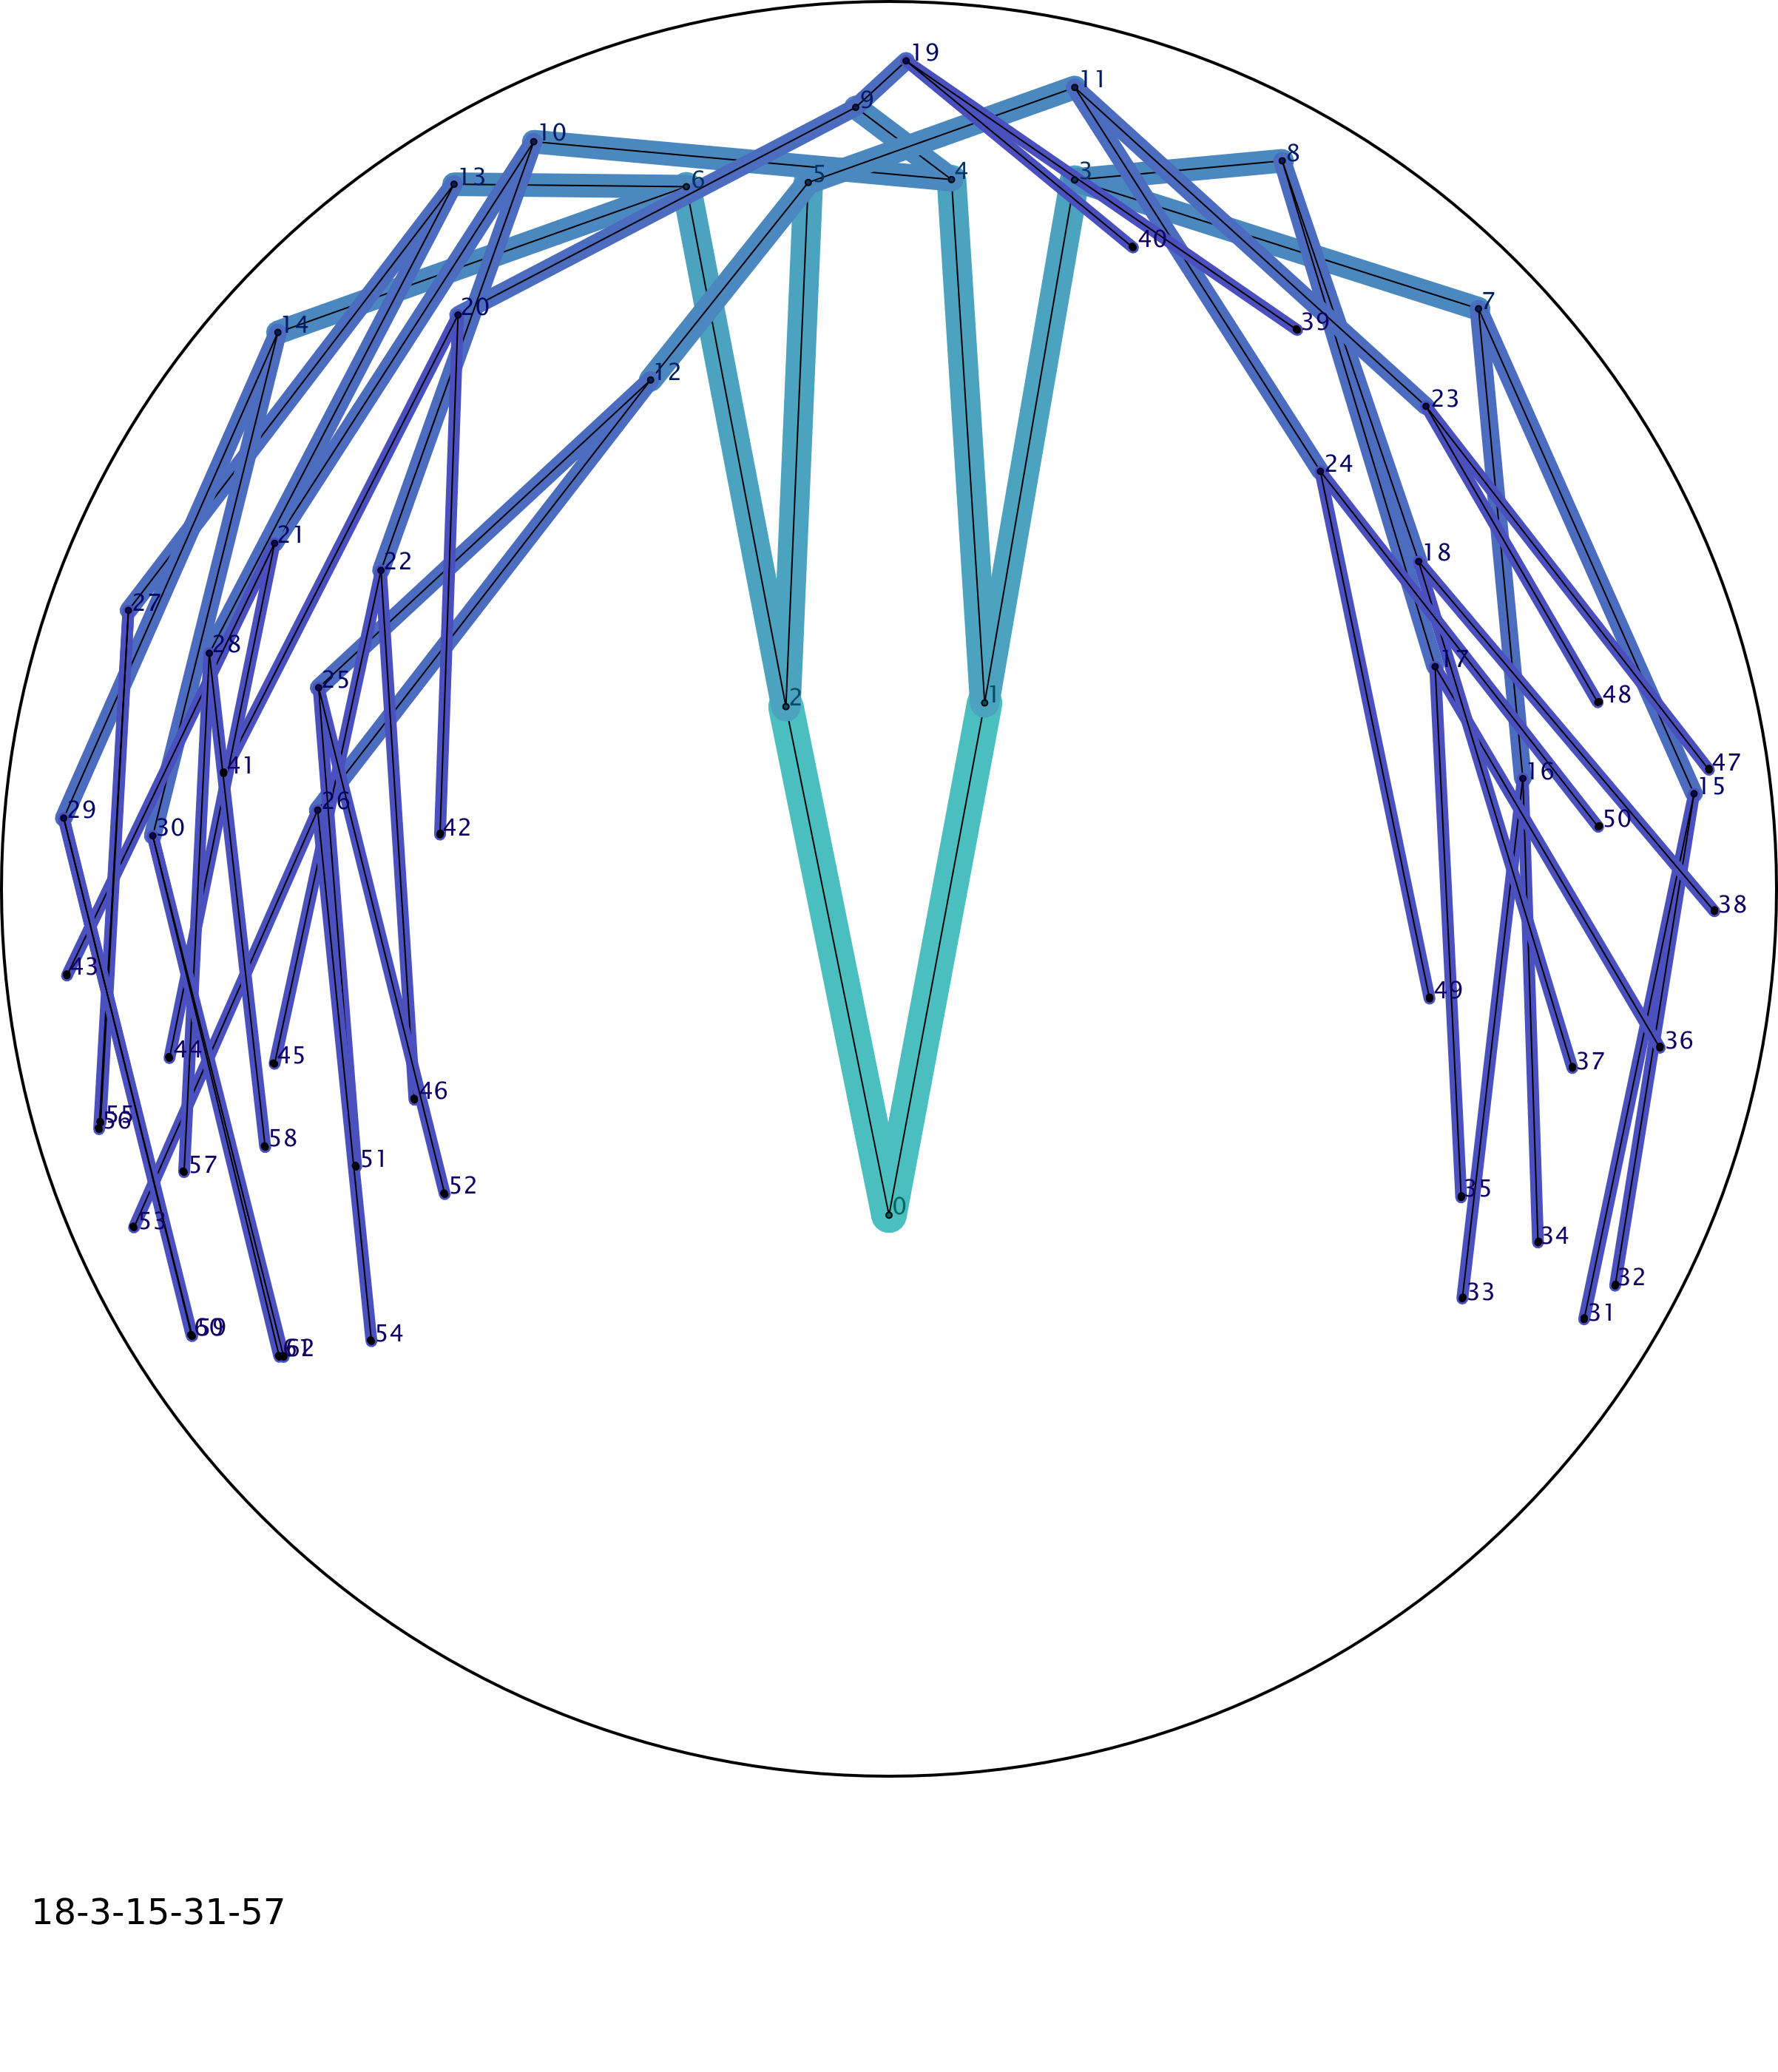
\includegraphics[width=\textwidth]{img_18-3-15-31-57}
\captionof{figure}{companyRadius = 120}
\end{minipage}
\hspace{0.5cm}
\begin{minipage}[t]{\imgSize\textwidth}
\raisebox{0.175\totalheight}{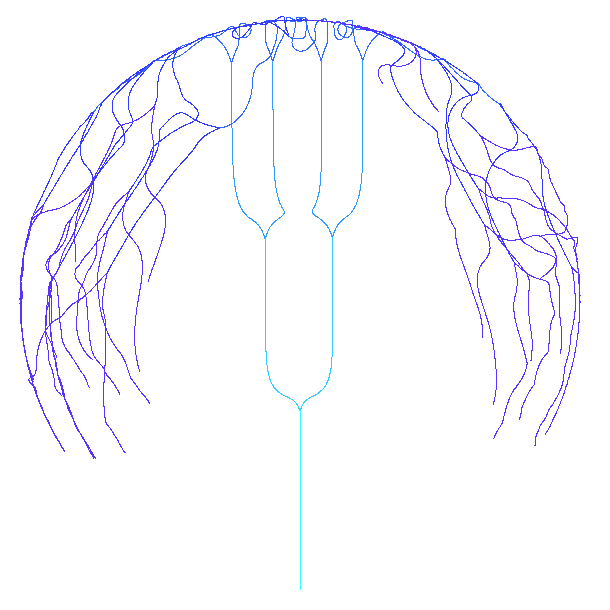
\includegraphics[width=\textwidth]{tank_companyRadius_trace_18-3-15-31-57_1}}
\captionof{figure}{companyRadius = 120}
\end{minipage}
\vspace{0.5cm}

\newpage
\subsubsection{Variations of "interpolationSpeed"}

%50
\begin{minipage}[t]{\imgSize\textwidth}
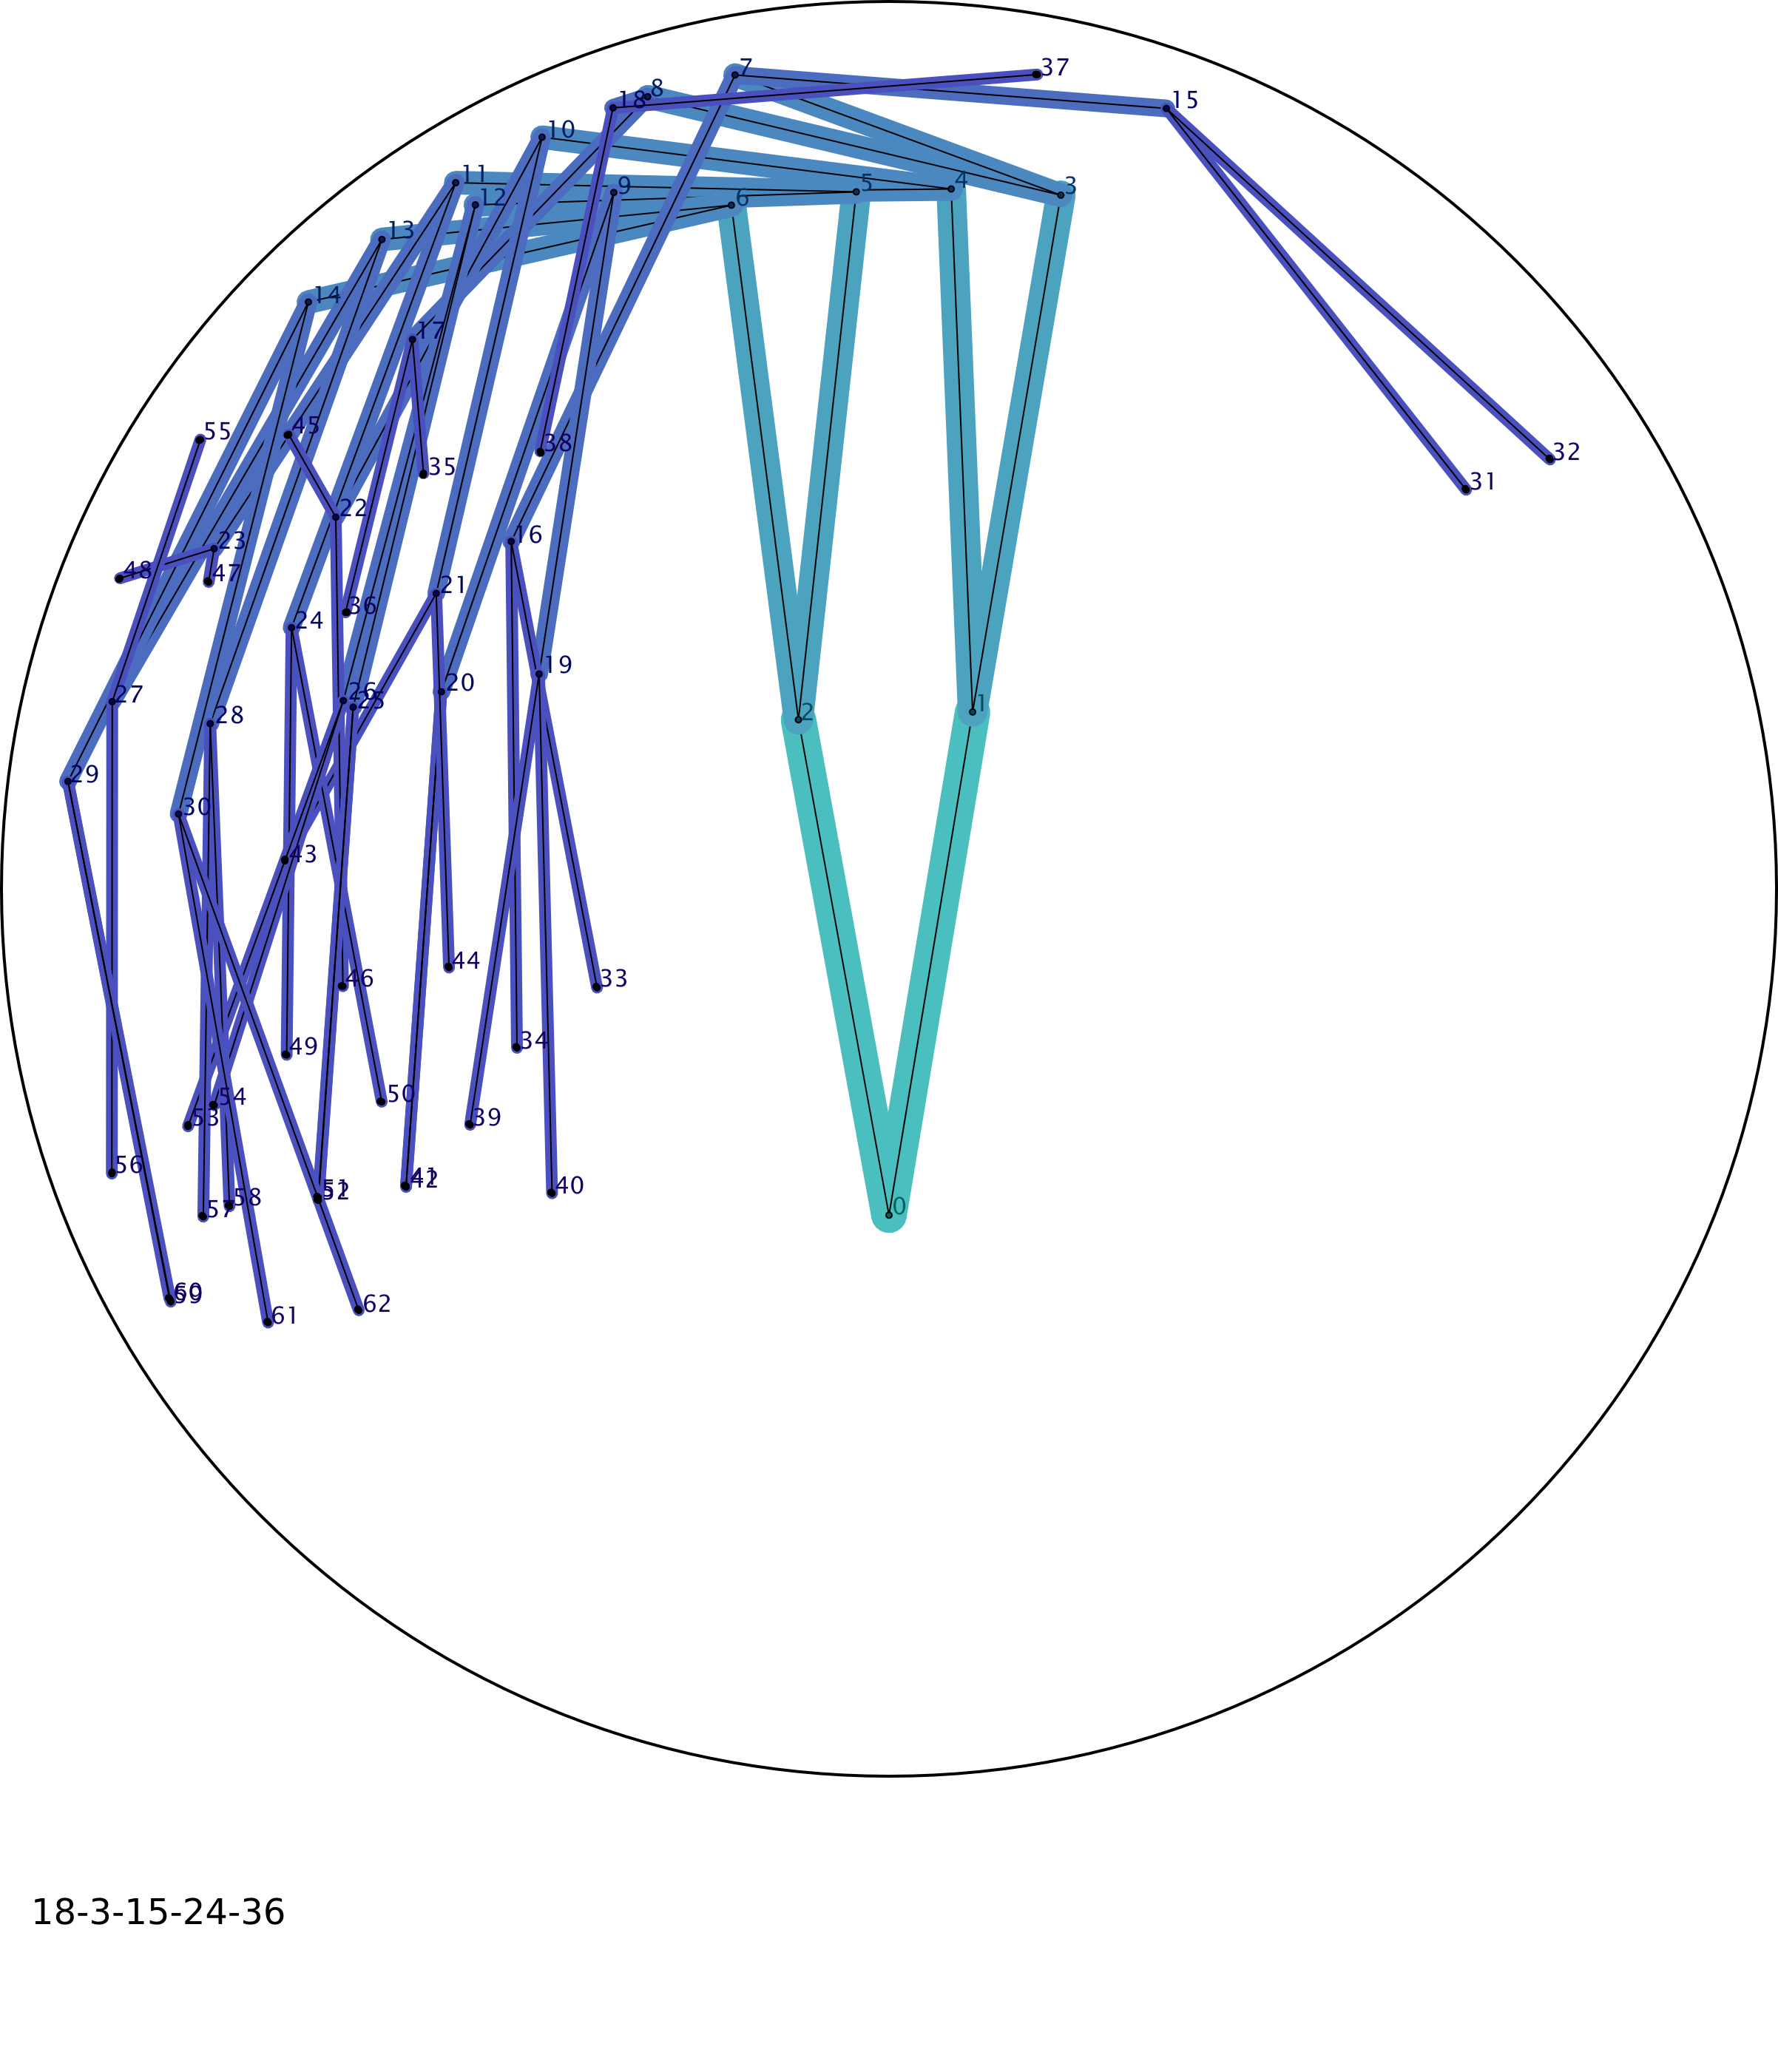
\includegraphics[width=\textwidth]{img_18-3-15-24-36}
\captionof{figure}{interpolationSpeed = 50}
\end{minipage}
\hspace{0.5cm}
\begin{minipage}[t]{\imgSize\textwidth}
\raisebox{0.175\totalheight}{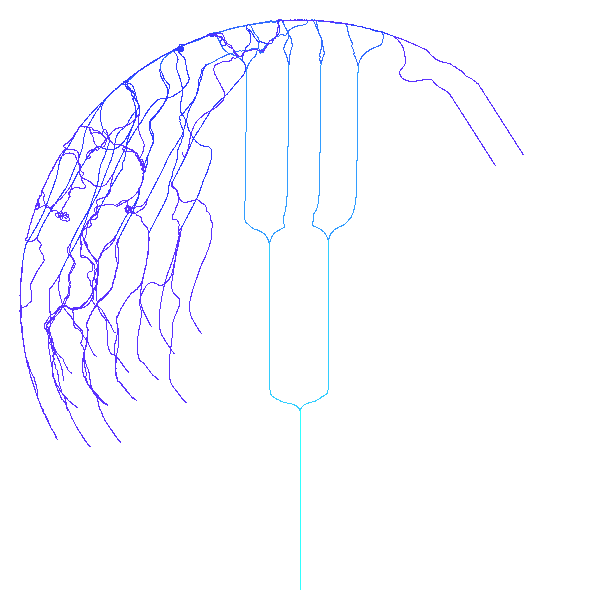
\includegraphics[width=\textwidth]{tank_interpolationSpeed_trace_18-3-15-24-36_1}}
\captionof{figure}{interpolationSpeed = 50}
\end{minipage}
\vspace{0.5cm} 

%100 def
\begin{minipage}[t]{\imgSize\textwidth}
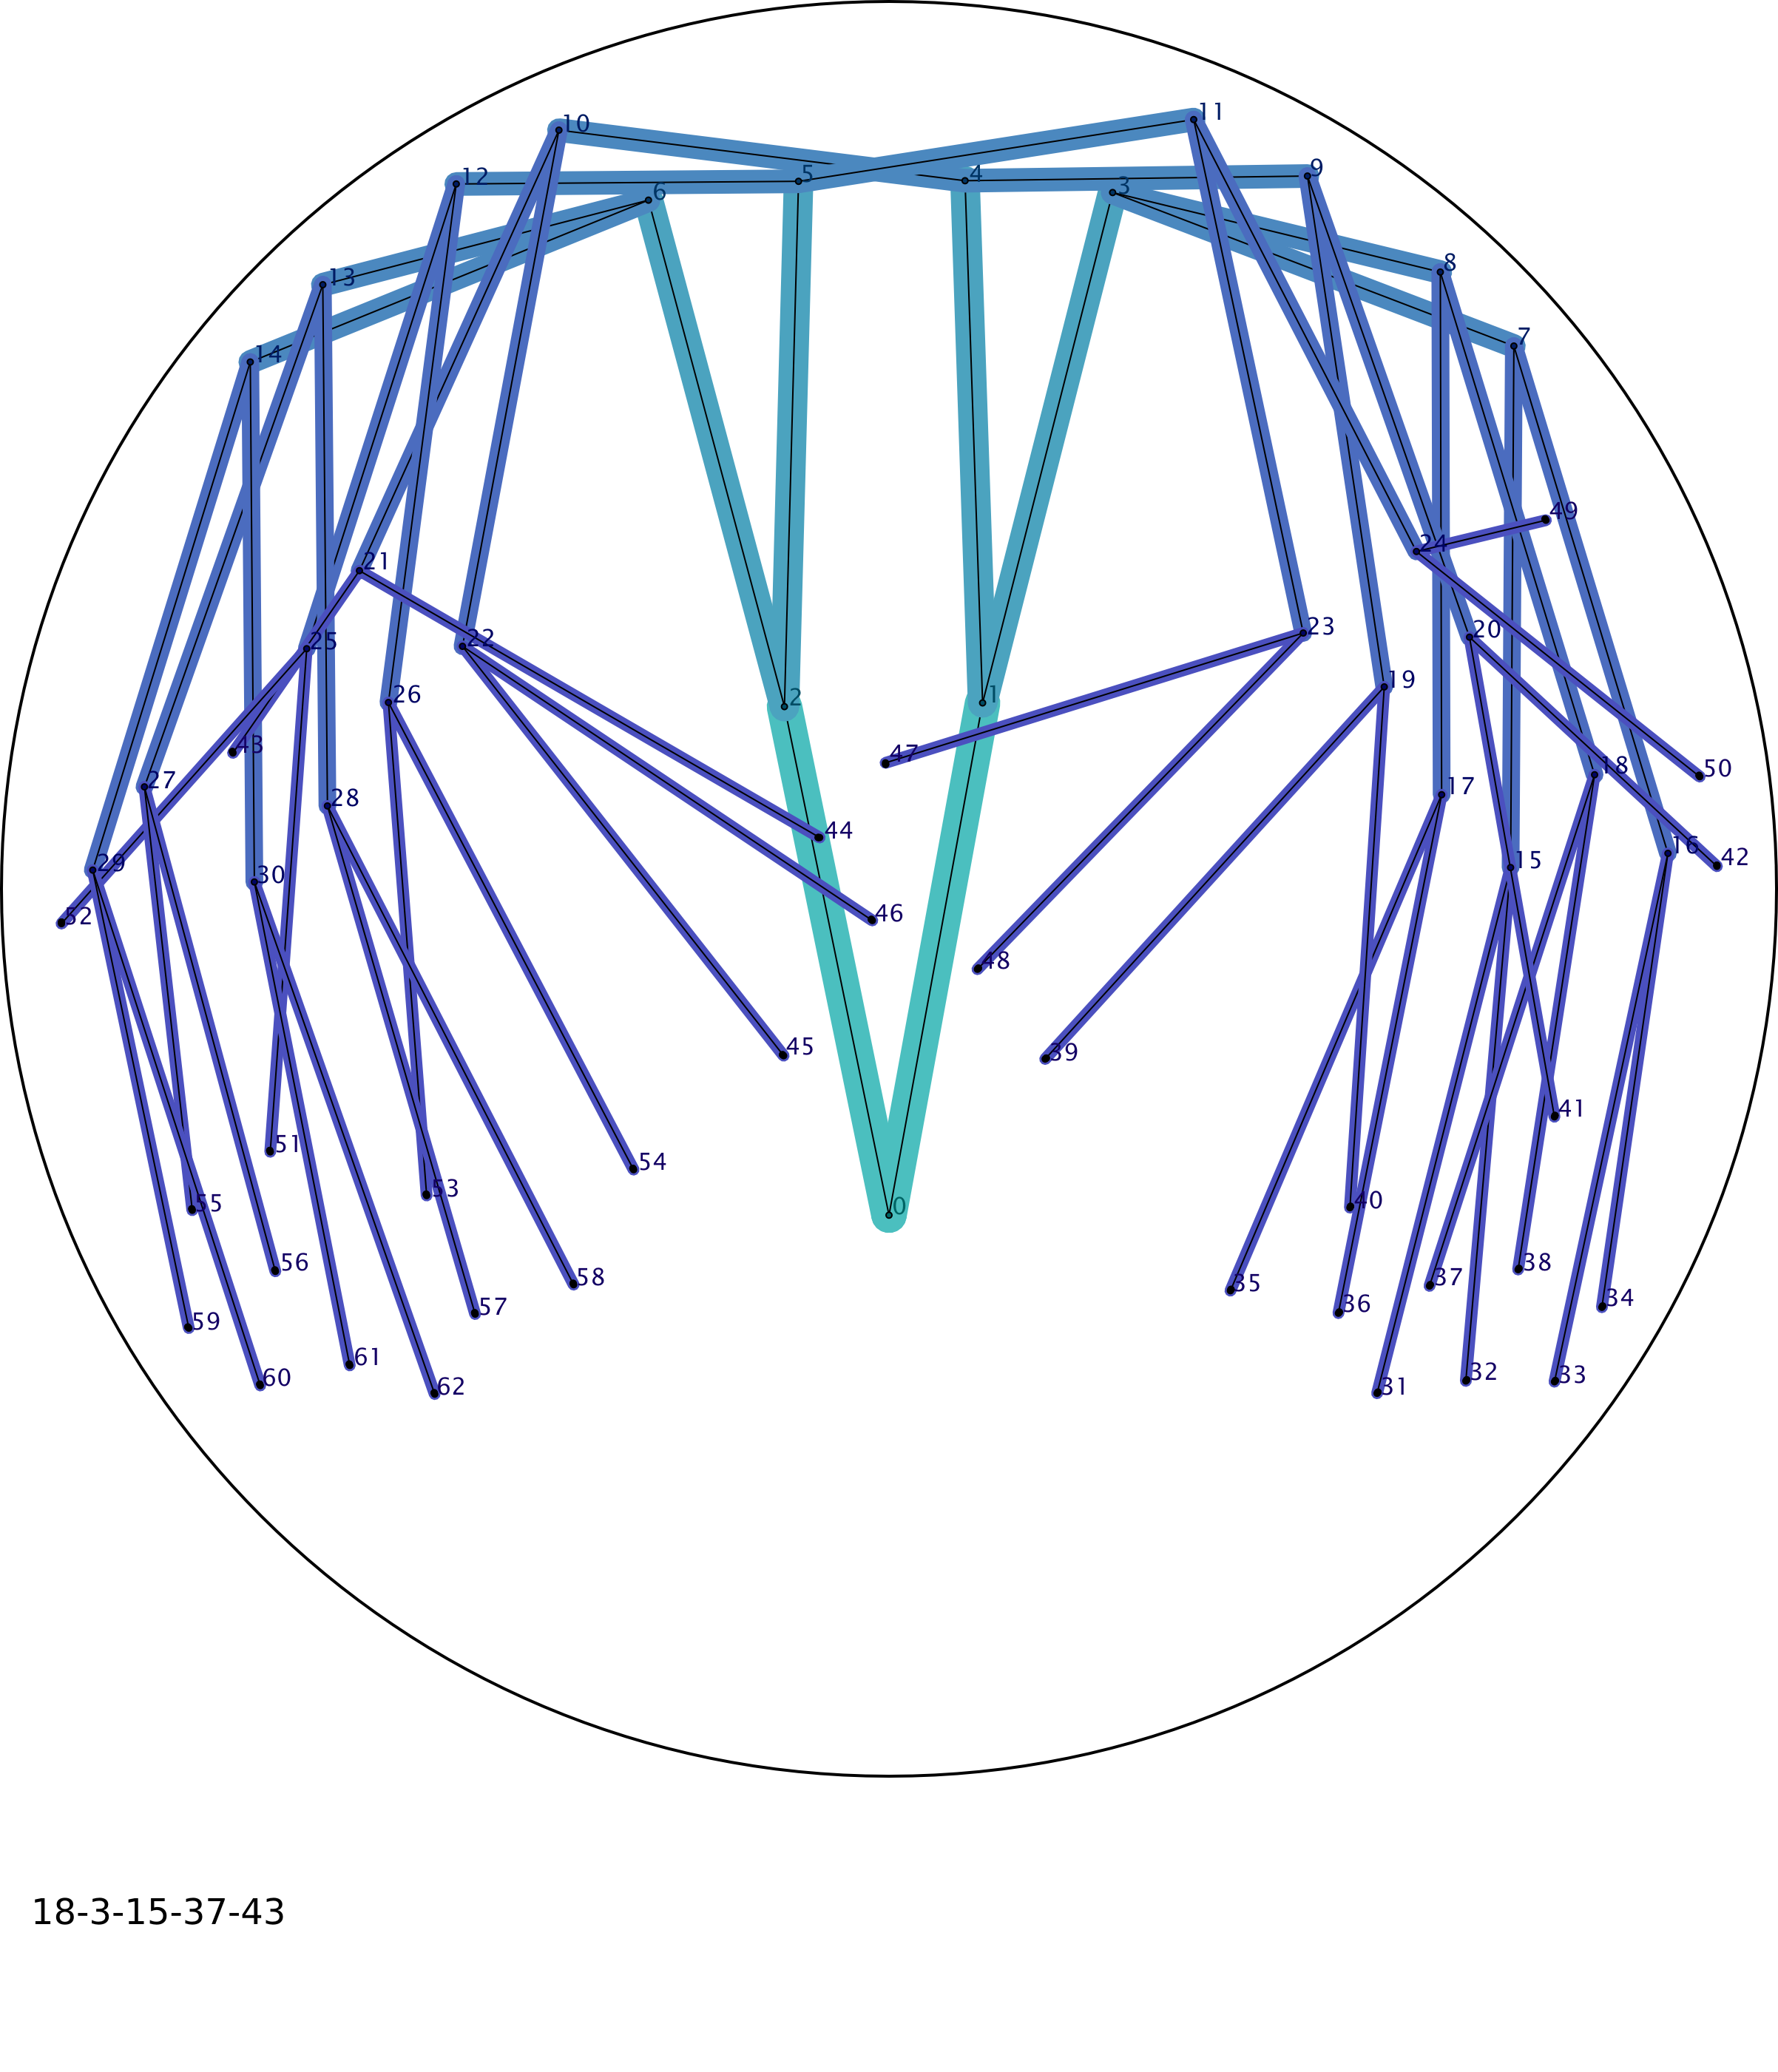
\includegraphics[width=\textwidth]{img_18-3-15-37-43}
\captionof{figure}{interpolationSpeed = 100 (default)}
\end{minipage}
\hspace{0.5cm}
\begin{minipage}[t]{\imgSize\textwidth}
\raisebox{0.175\totalheight}{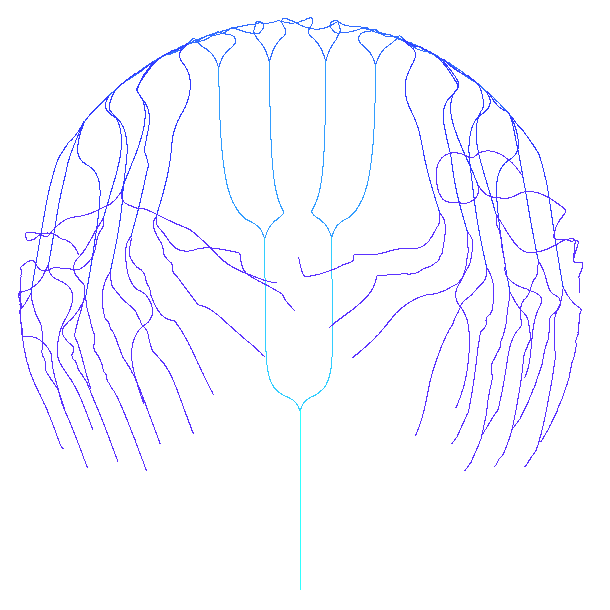
\includegraphics[width=\textwidth]{tank_default_trace_18-3-15-37-43_1}}
\captionof{figure}{interpolationSpeed = 100 (default)}
\end{minipage}
\vspace{0.5cm}

%150
\begin{minipage}[t]{\imgSize\textwidth}
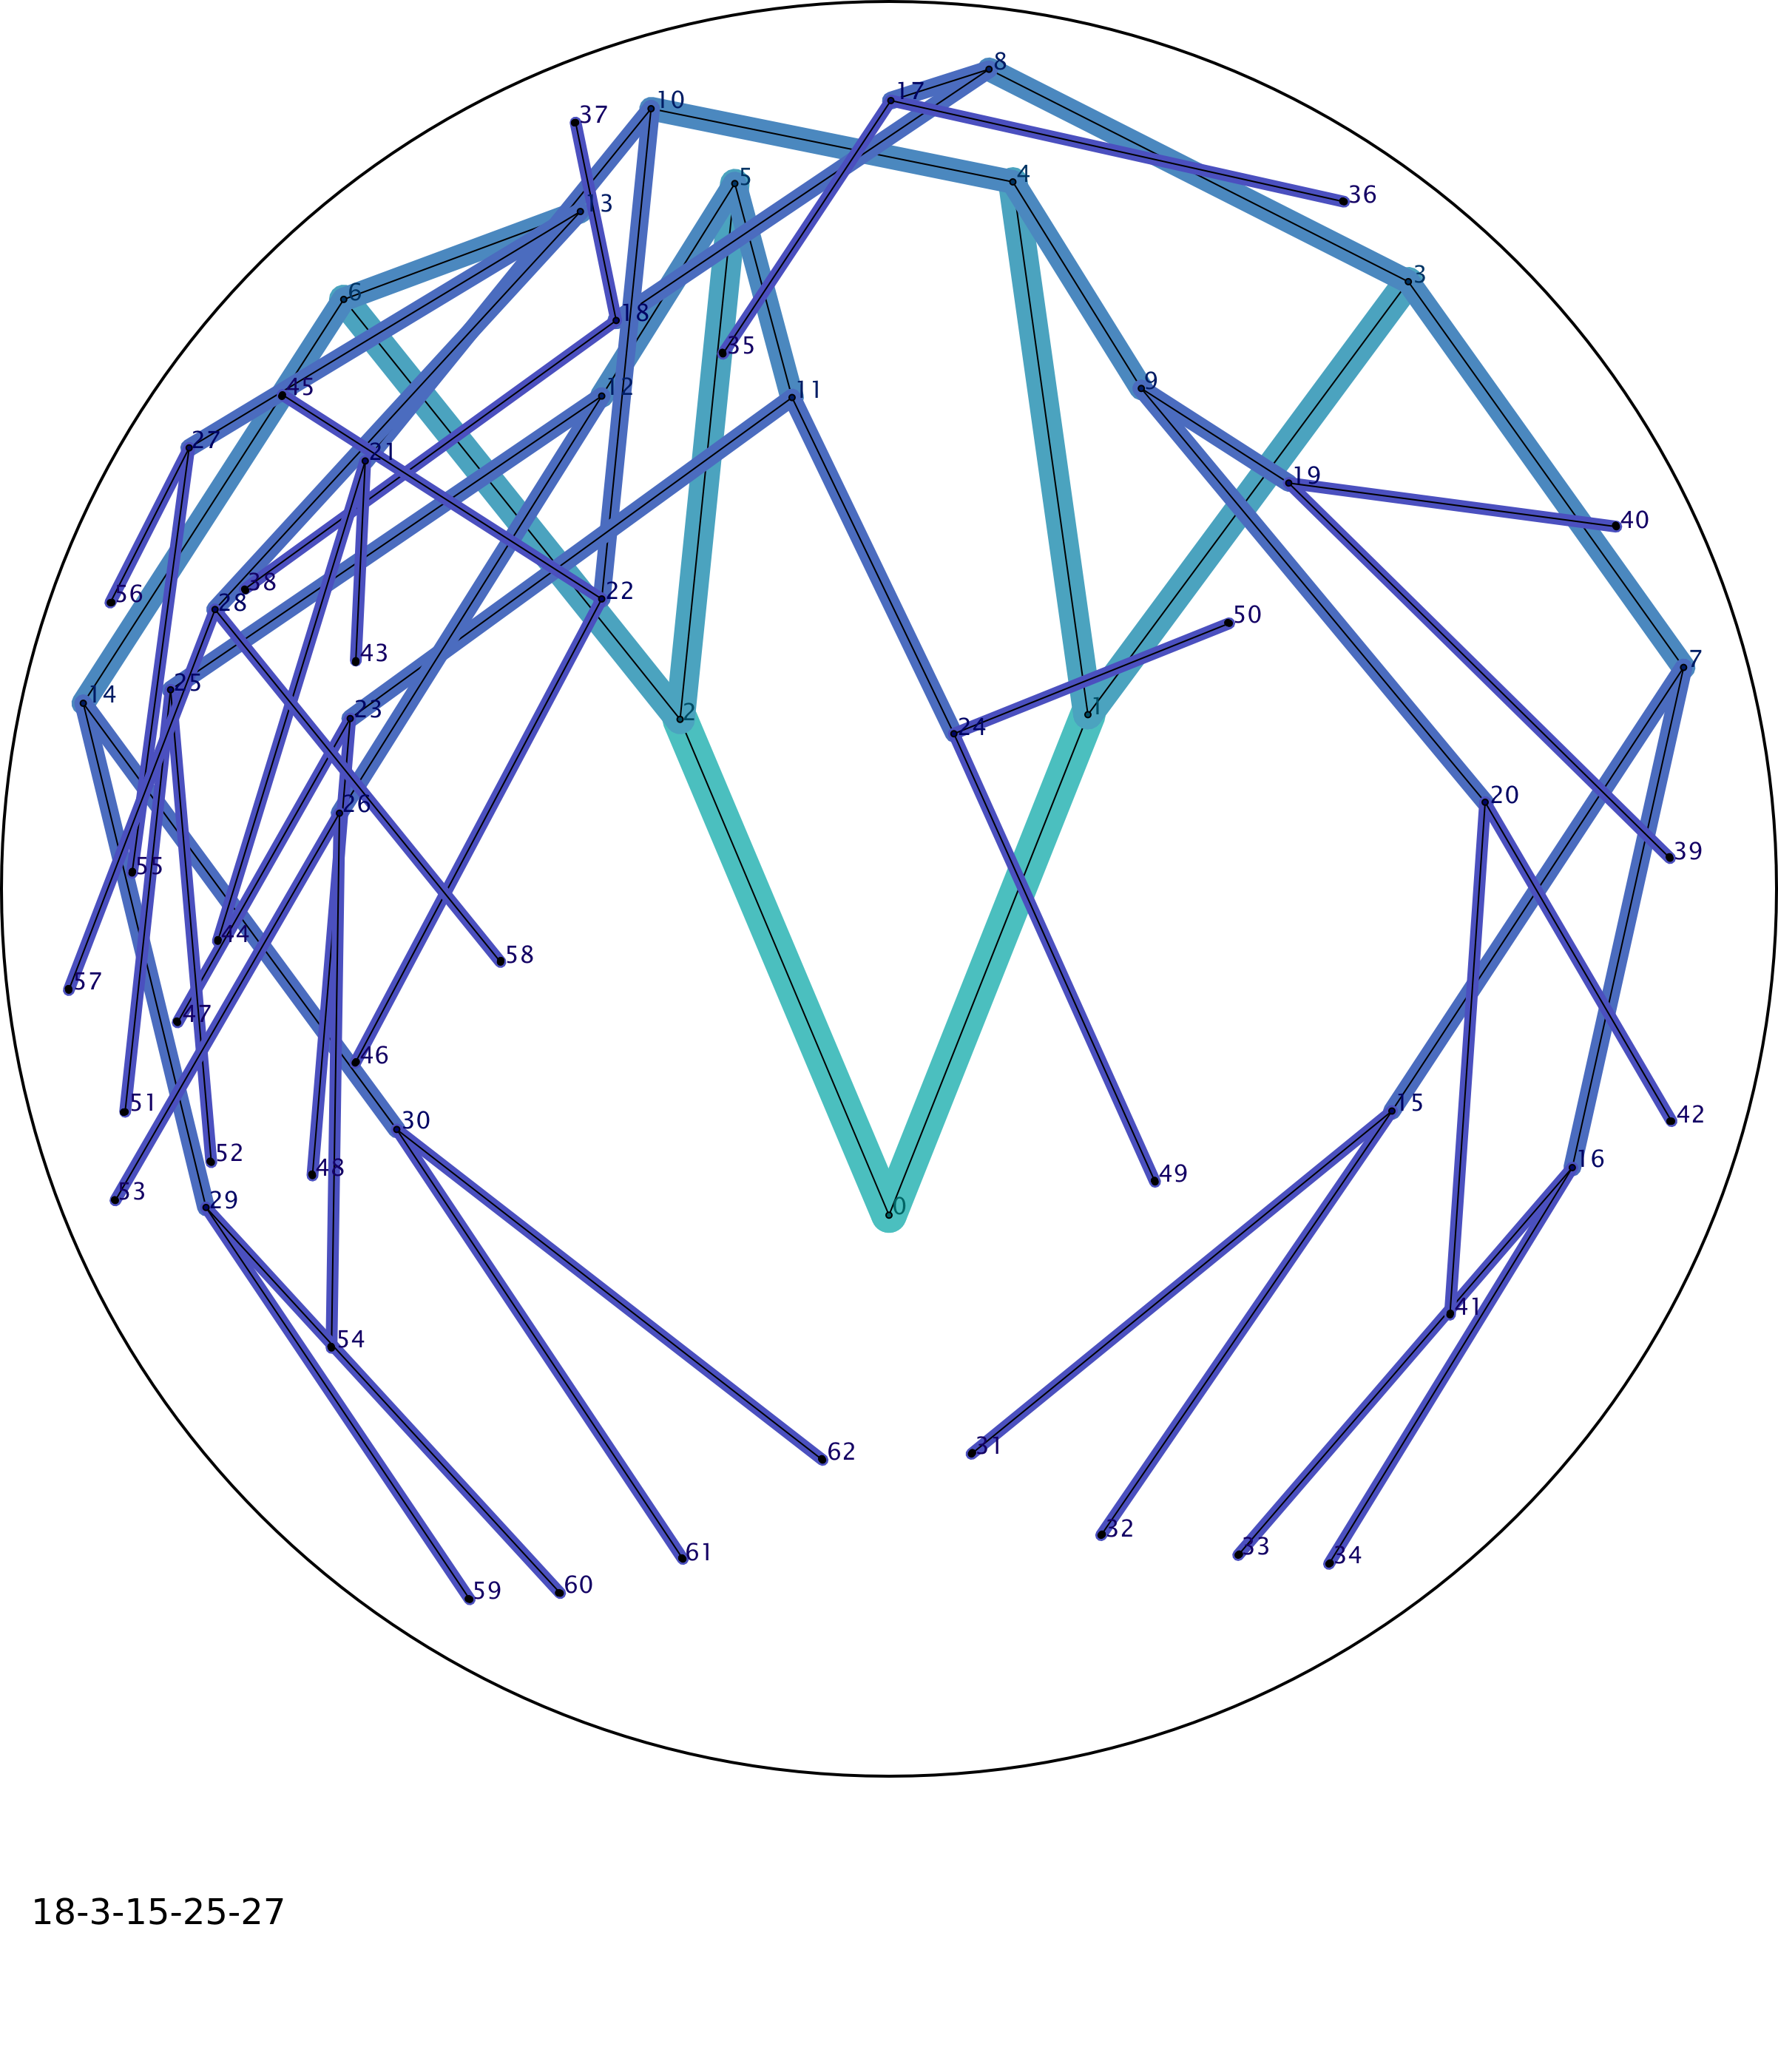
\includegraphics[width=\textwidth]{img_18-3-15-25-27}
\captionof{figure}{interpolationSpeed = 150}
\end{minipage}
\hspace{0.5cm}
\begin{minipage}[t]{\imgSize\textwidth}
\raisebox{0.175\totalheight}{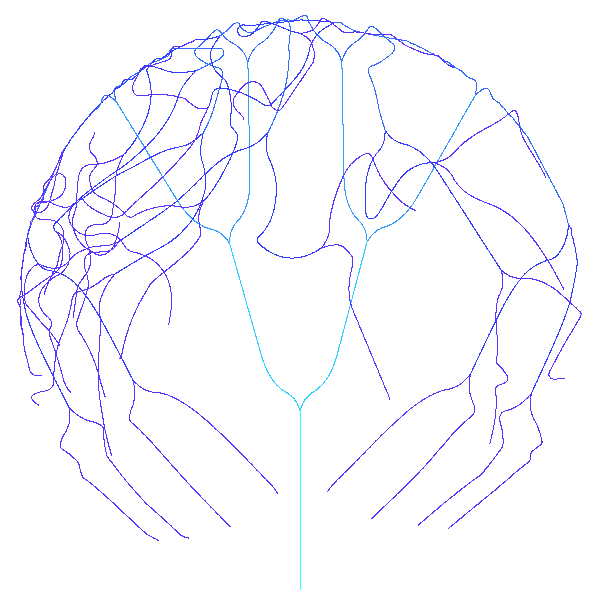
\includegraphics[width=\textwidth]{tank_interpolationSpeed_trace_18-3-15-25-27_1}}
\captionof{figure}{interpolationSpeed = 150}
\end{minipage}
\vspace{0.5cm}

%200
\begin{minipage}[t]{\imgSize\textwidth}
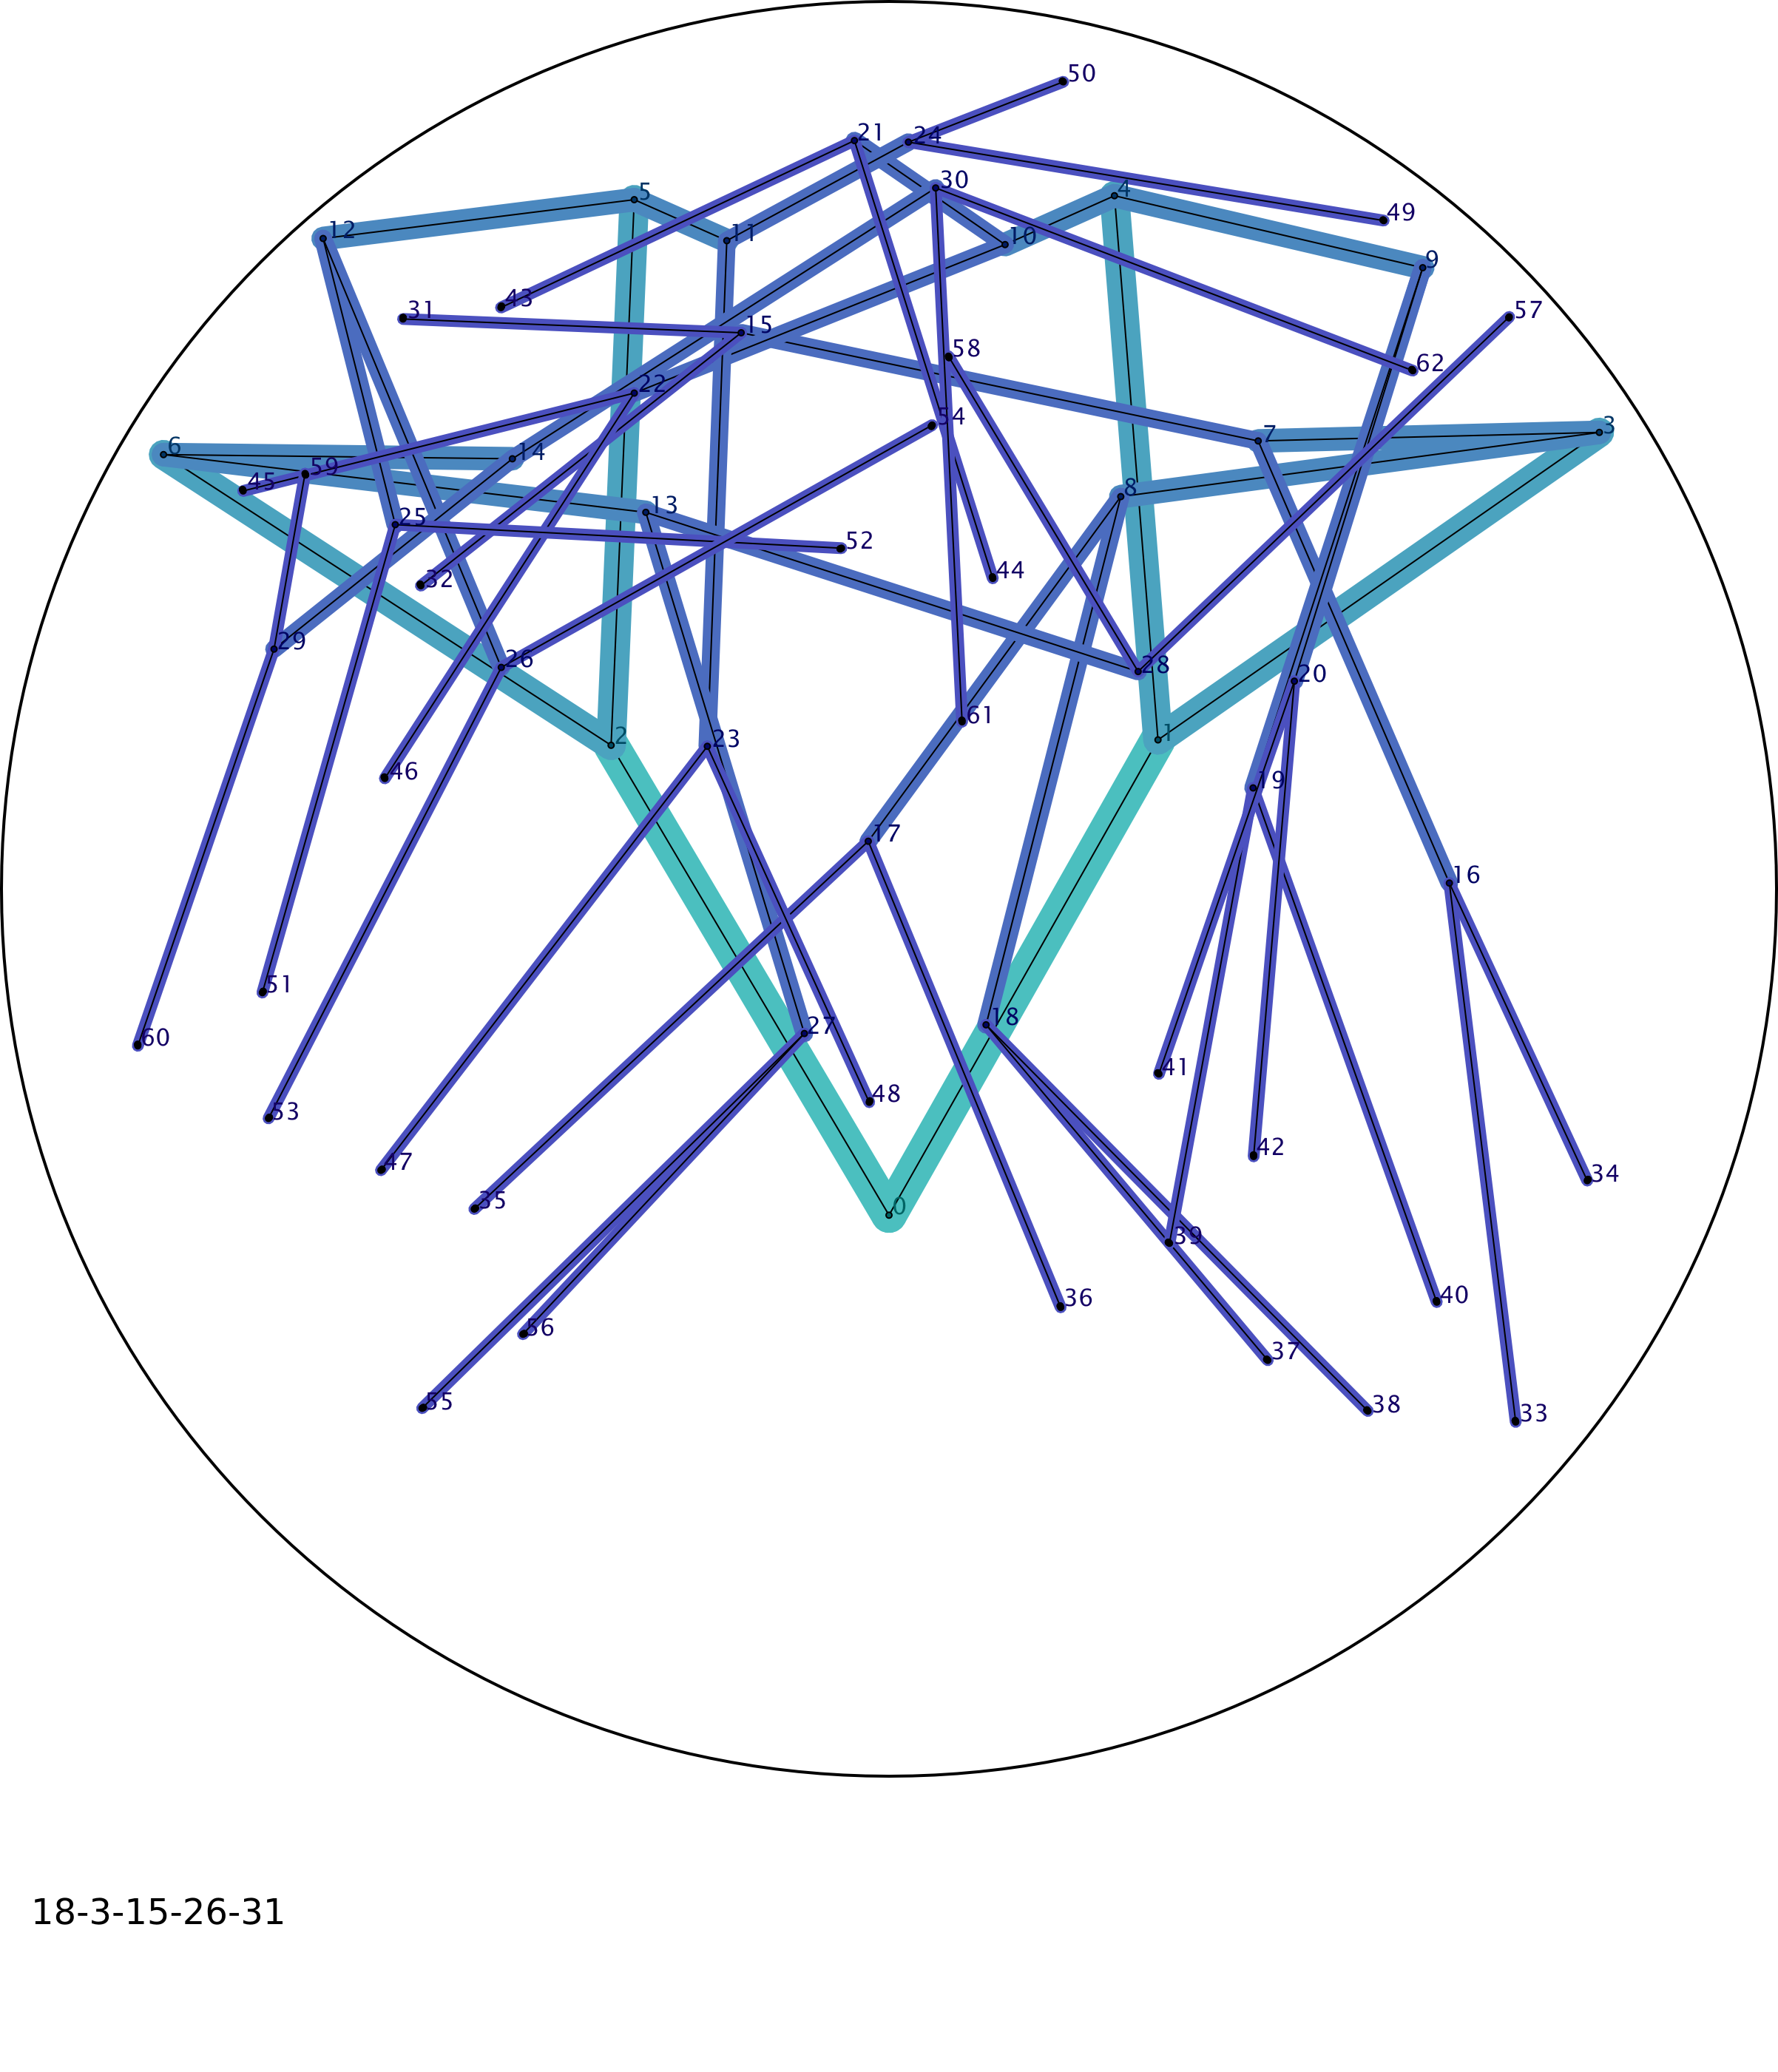
\includegraphics[width=\textwidth]{img_18-3-15-26-31}
\captionof{figure}{interpolationSpeed = 200}
\end{minipage}
\hspace{0.5cm}
\begin{minipage}[t]{\imgSize\textwidth}
\raisebox{0.175\totalheight}{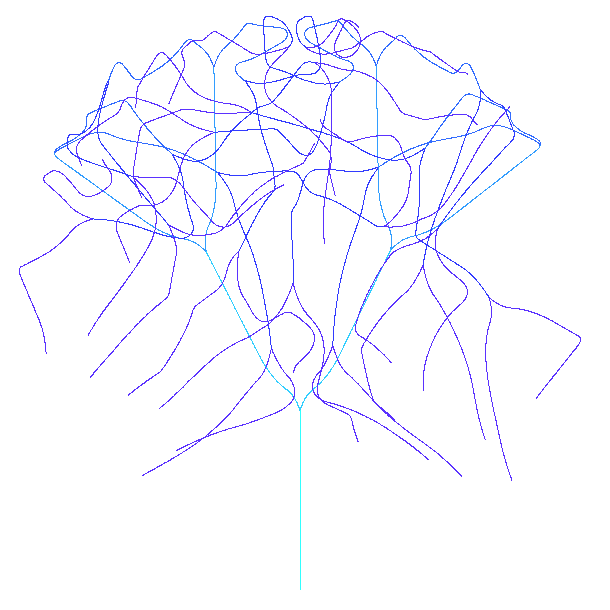
\includegraphics[width=\textwidth]{tank_interpolationSpeed_trace_18-3-15-26-31_1}}
\captionof{figure}{interpolationSpeed = 200}
\end{minipage}
\vspace{0.5cm}

%250
\begin{minipage}[t]{\imgSize\textwidth}
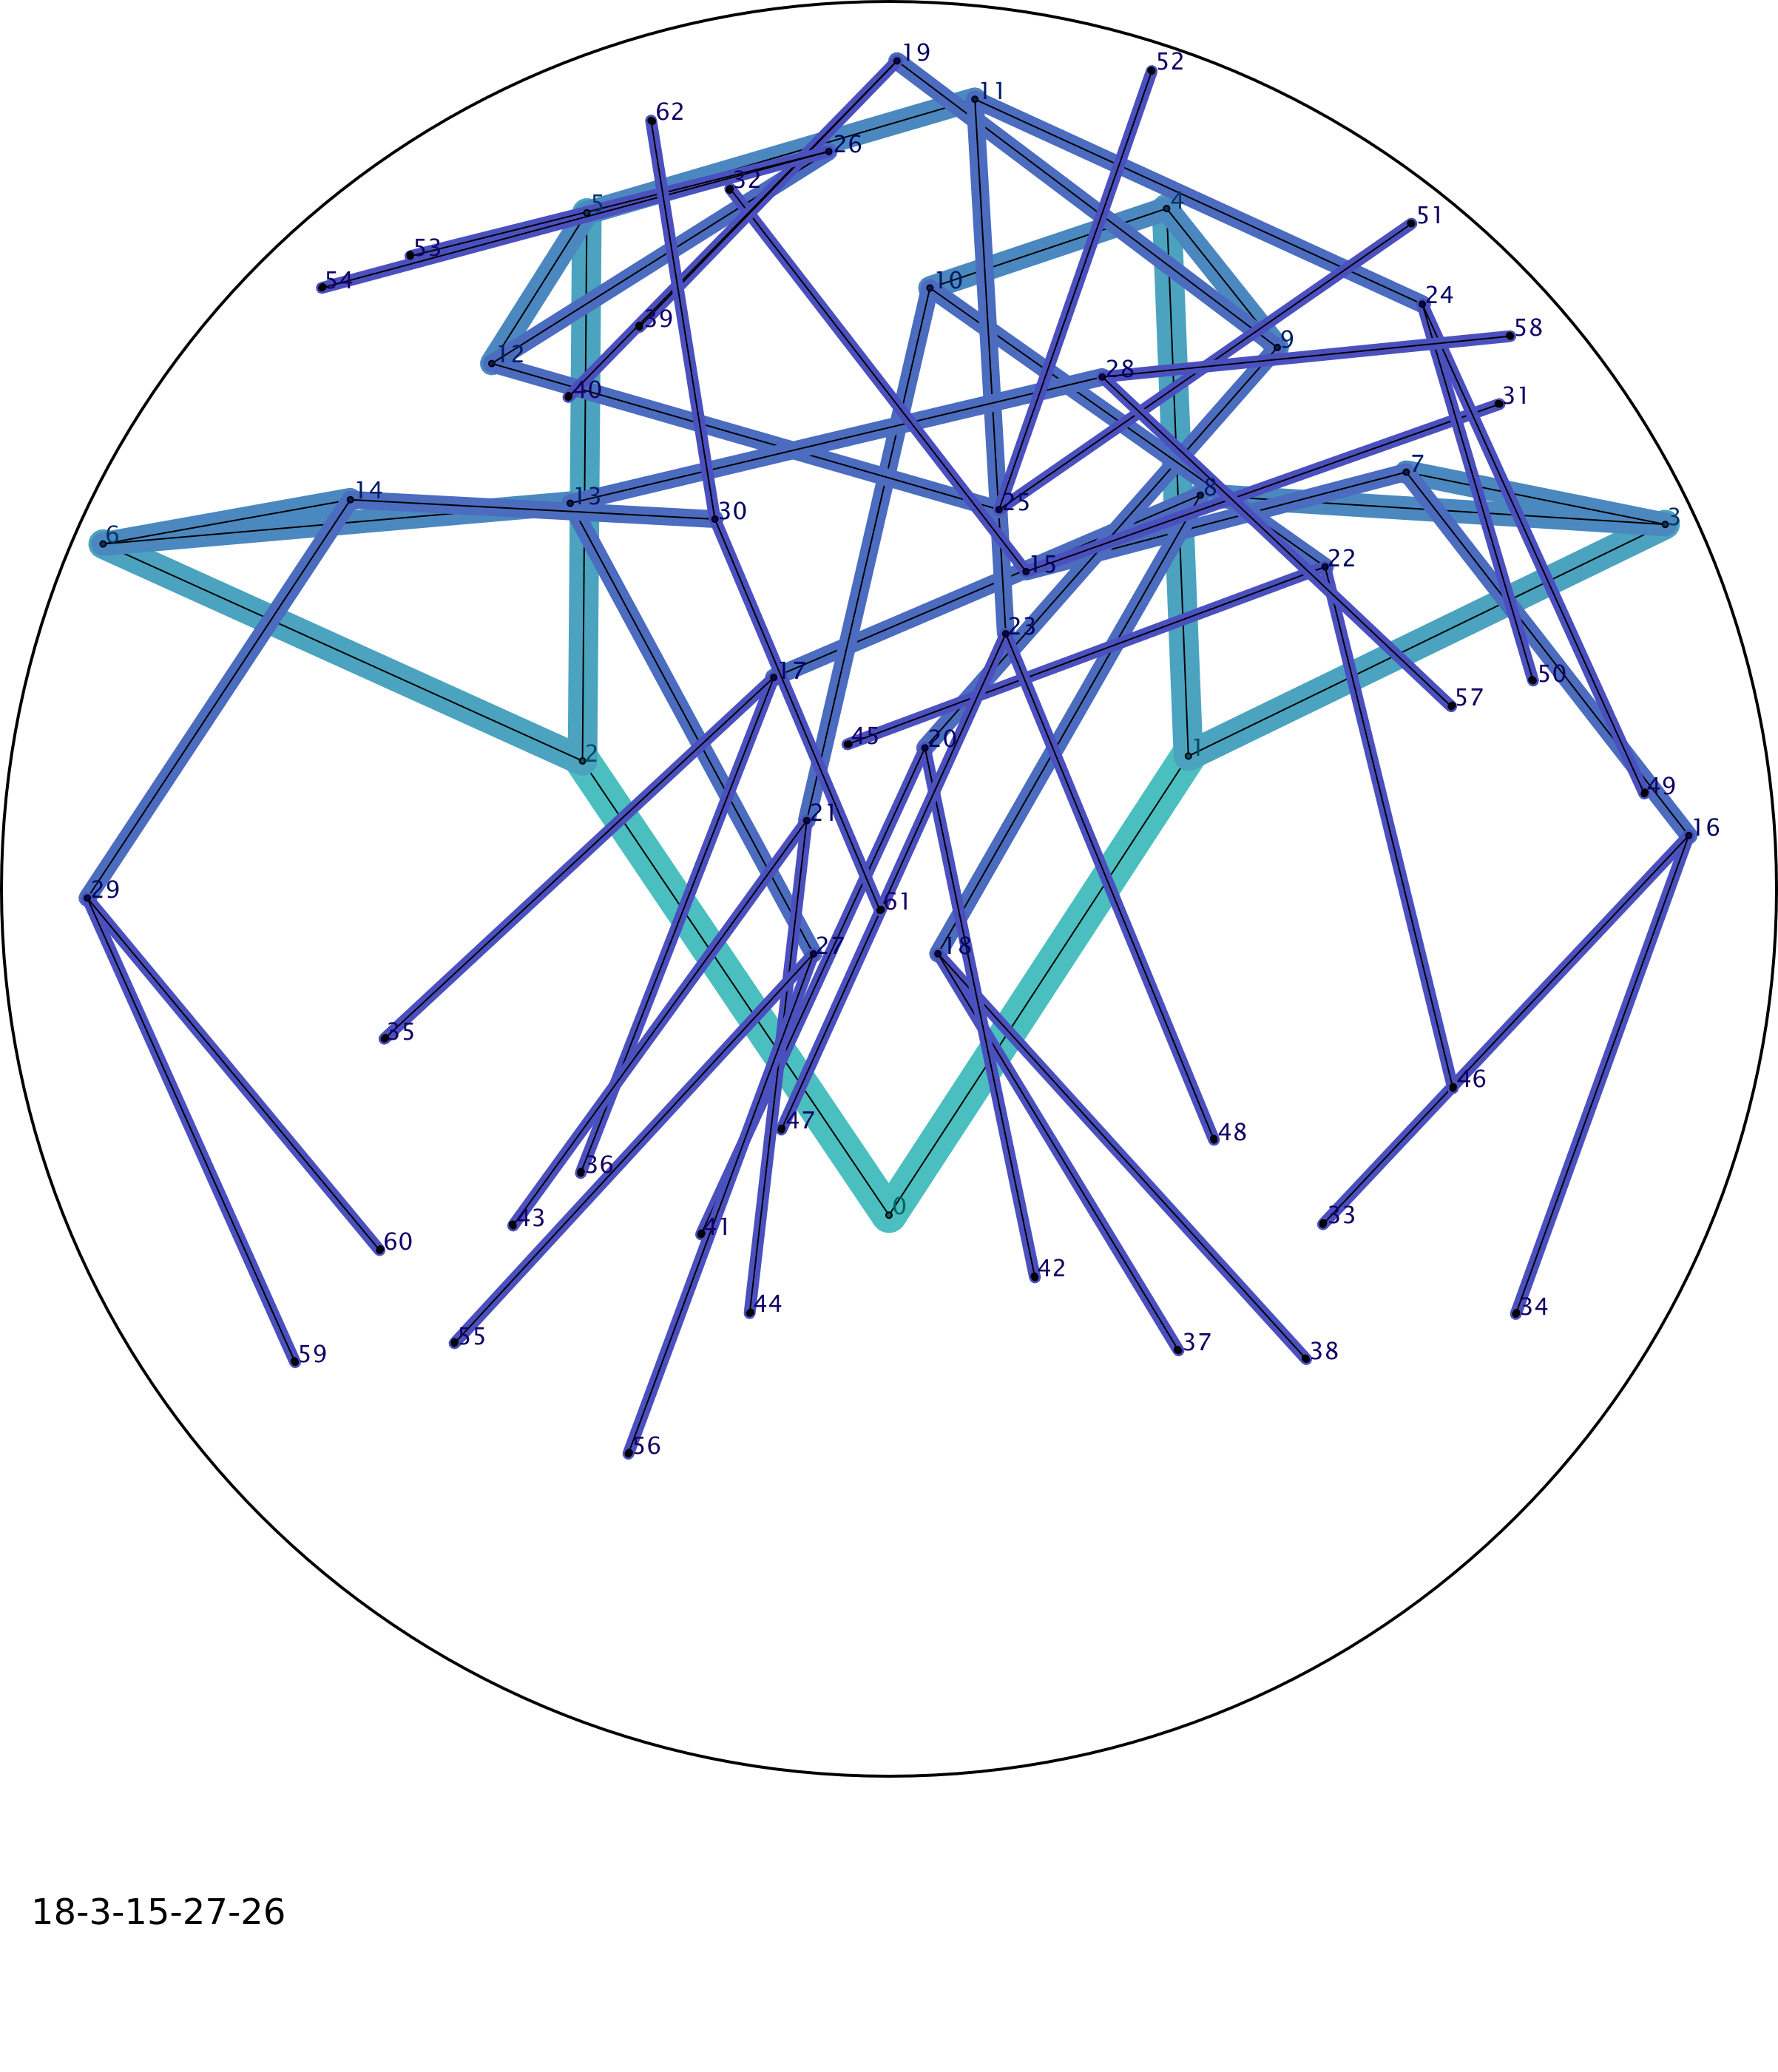
\includegraphics[width=\textwidth]{img_18-3-15-27-26}
\captionof{figure}{interpolationSpeed = 250}
\end{minipage}
\hspace{0.5cm}
\begin{minipage}[t]{\imgSize\textwidth}
\raisebox{0.175\totalheight}{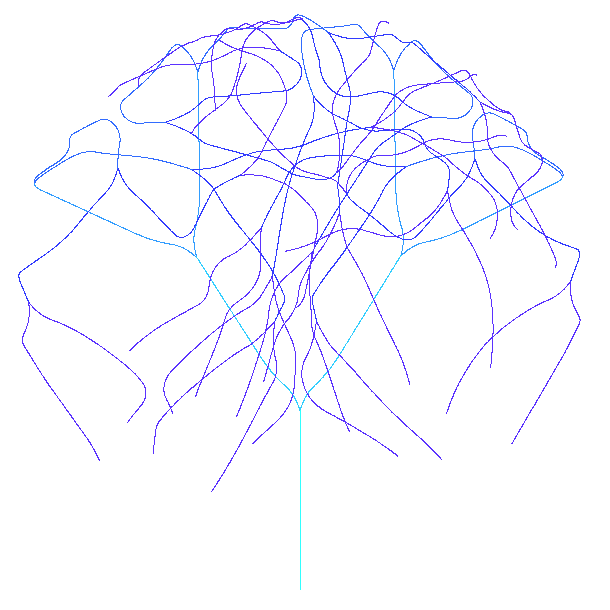
\includegraphics[width=\textwidth]{tank_interpolationSpeed_trace_18-3-15-27-26_1}}
\captionof{figure}{interpolationSpeed = 250}
\end{minipage}
\vspace{0.5cm}

%350
\begin{minipage}[t]{\imgSize\textwidth}
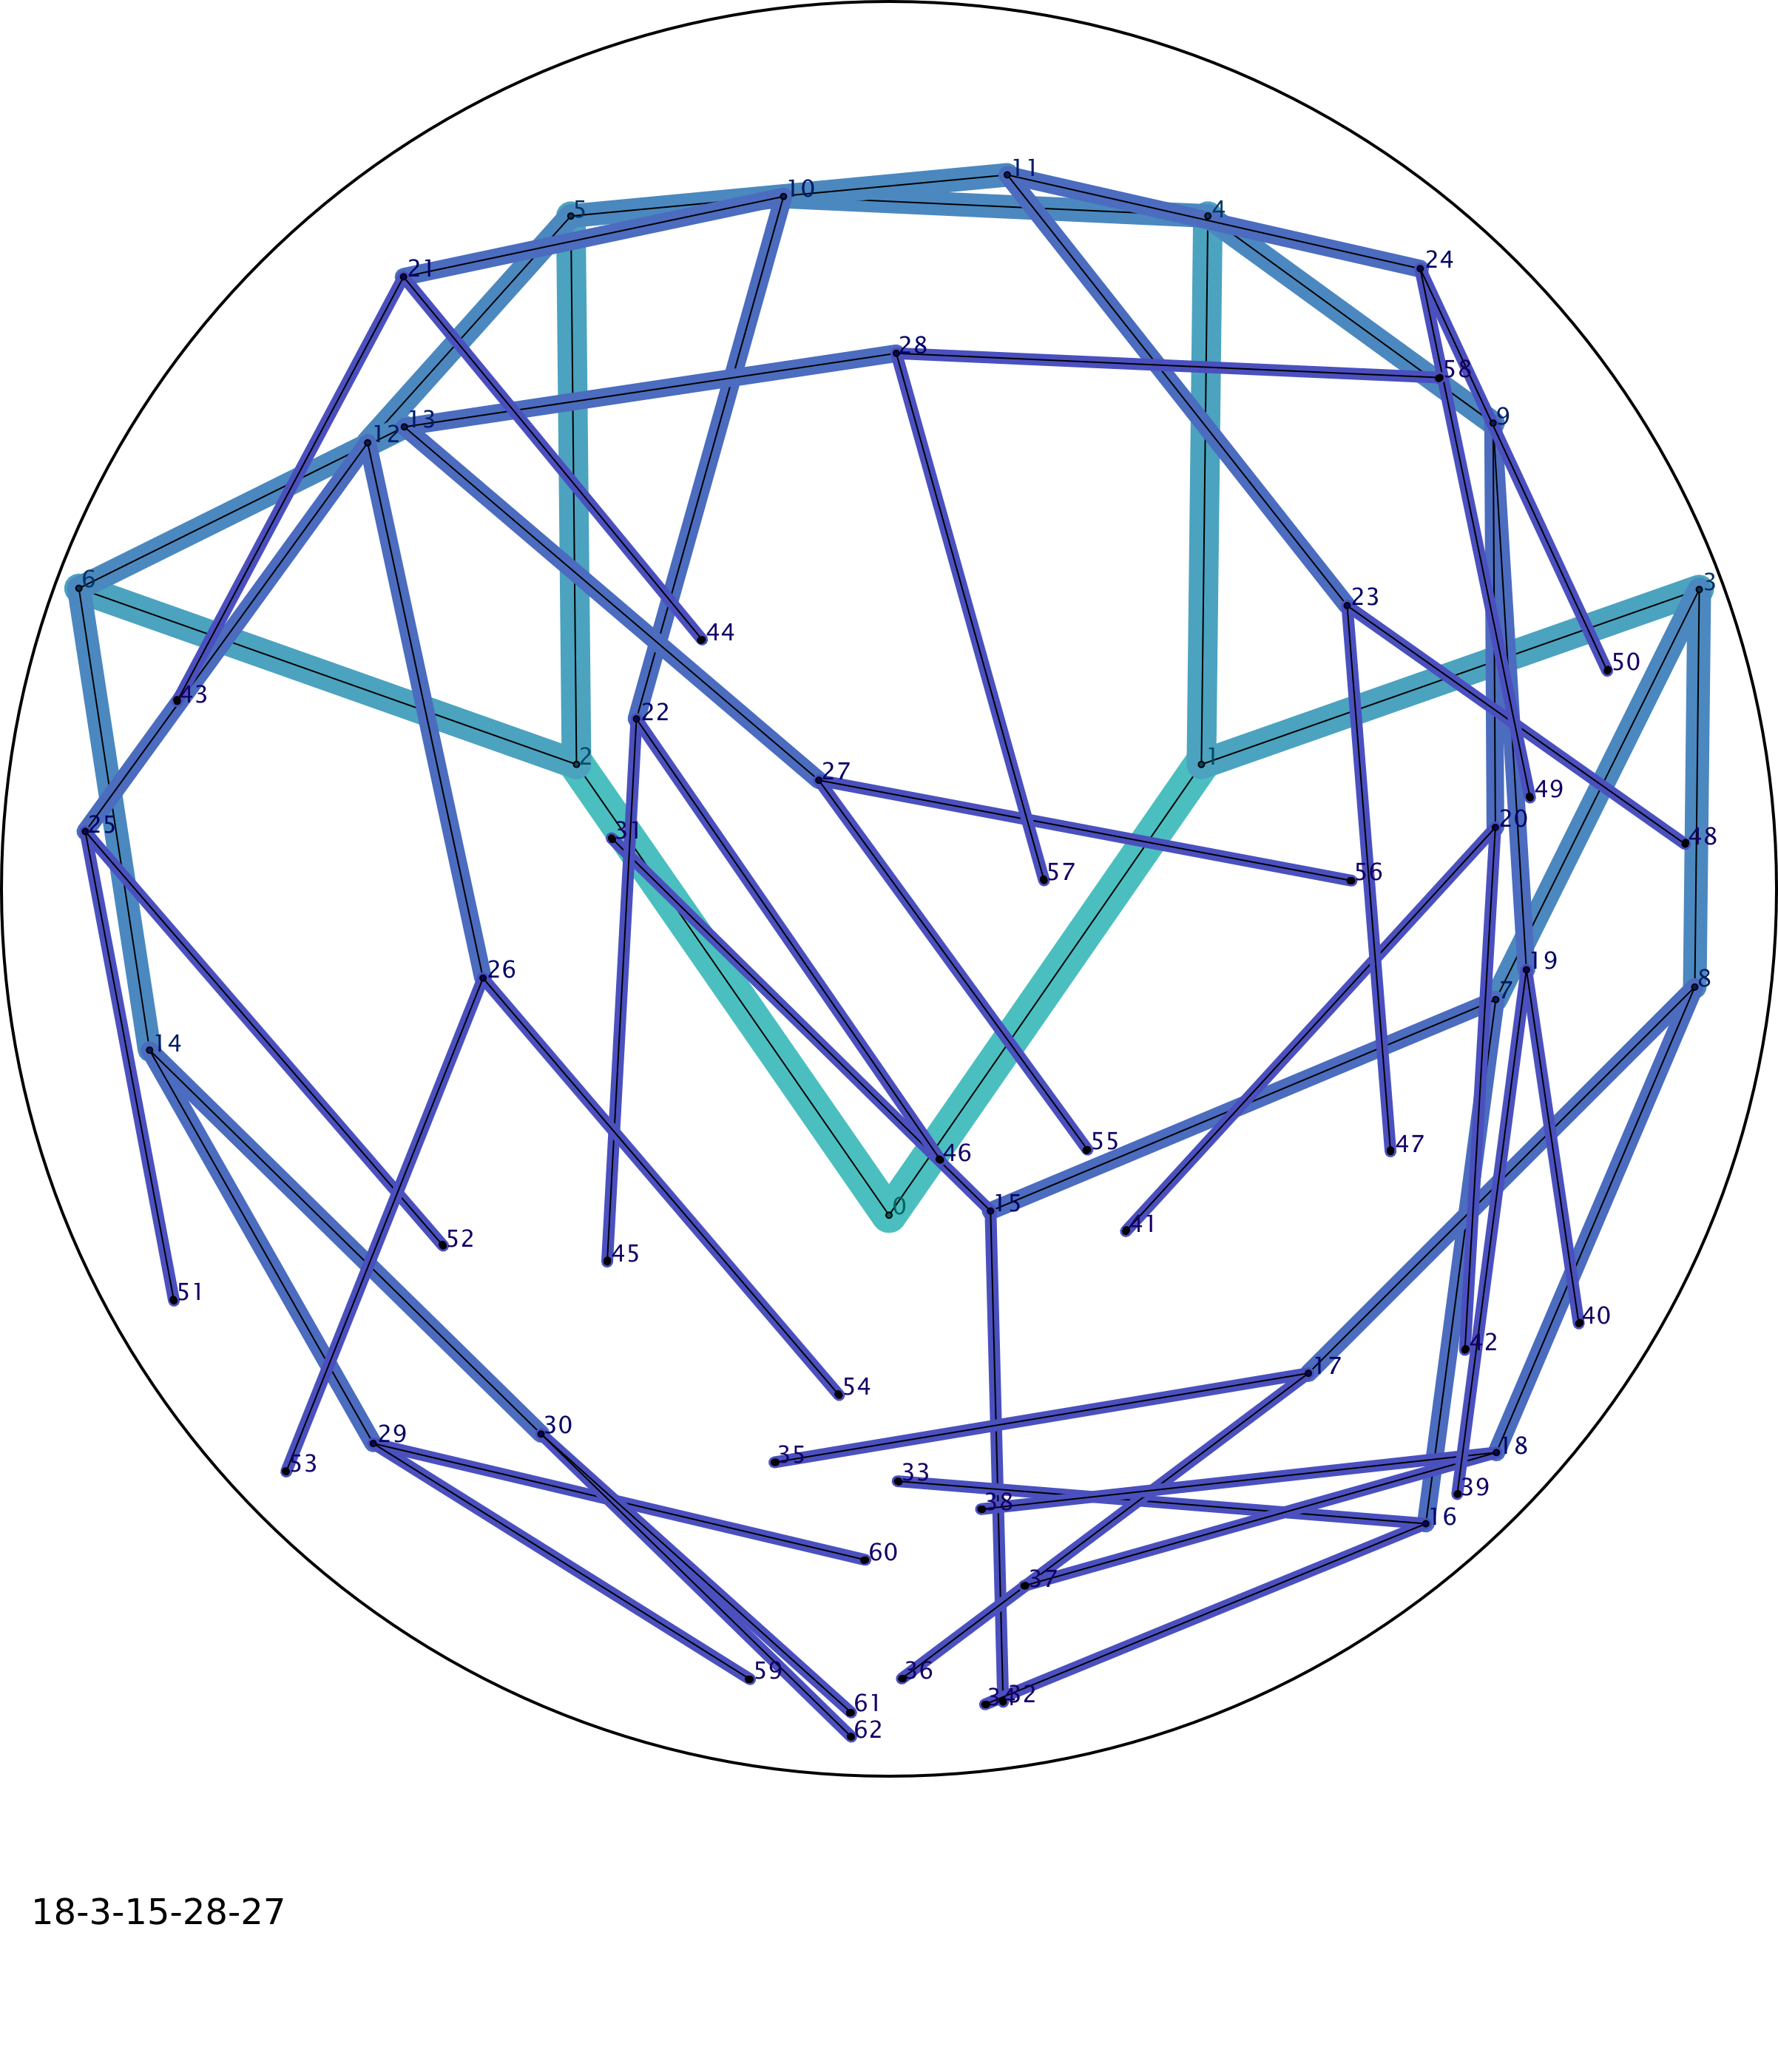
\includegraphics[width=\textwidth]{img_18-3-15-28-27}
\captionof{figure}{interpolationSpeed = 350}
\end{minipage}
\hspace{0.5cm}
\begin{minipage}[t]{\imgSize\textwidth}
\raisebox{0.175\totalheight}{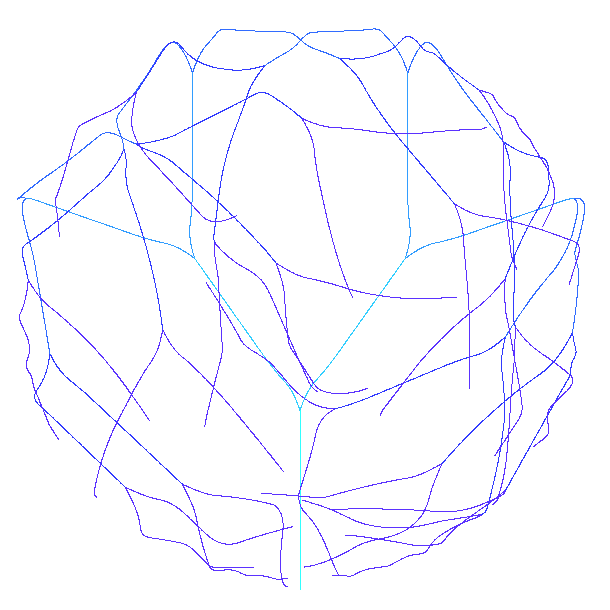
\includegraphics[width=\textwidth]{tank_interpolationSpeed_trace_18-3-15-28-27_1}}
\captionof{figure}{interpolationSpeed = 350}
\end{minipage}
\vspace{0.5cm}

\newpage
\subsubsection{Variations of "timetoSpawn"}

%3000
\begin{minipage}[t]{\imgSize\textwidth}
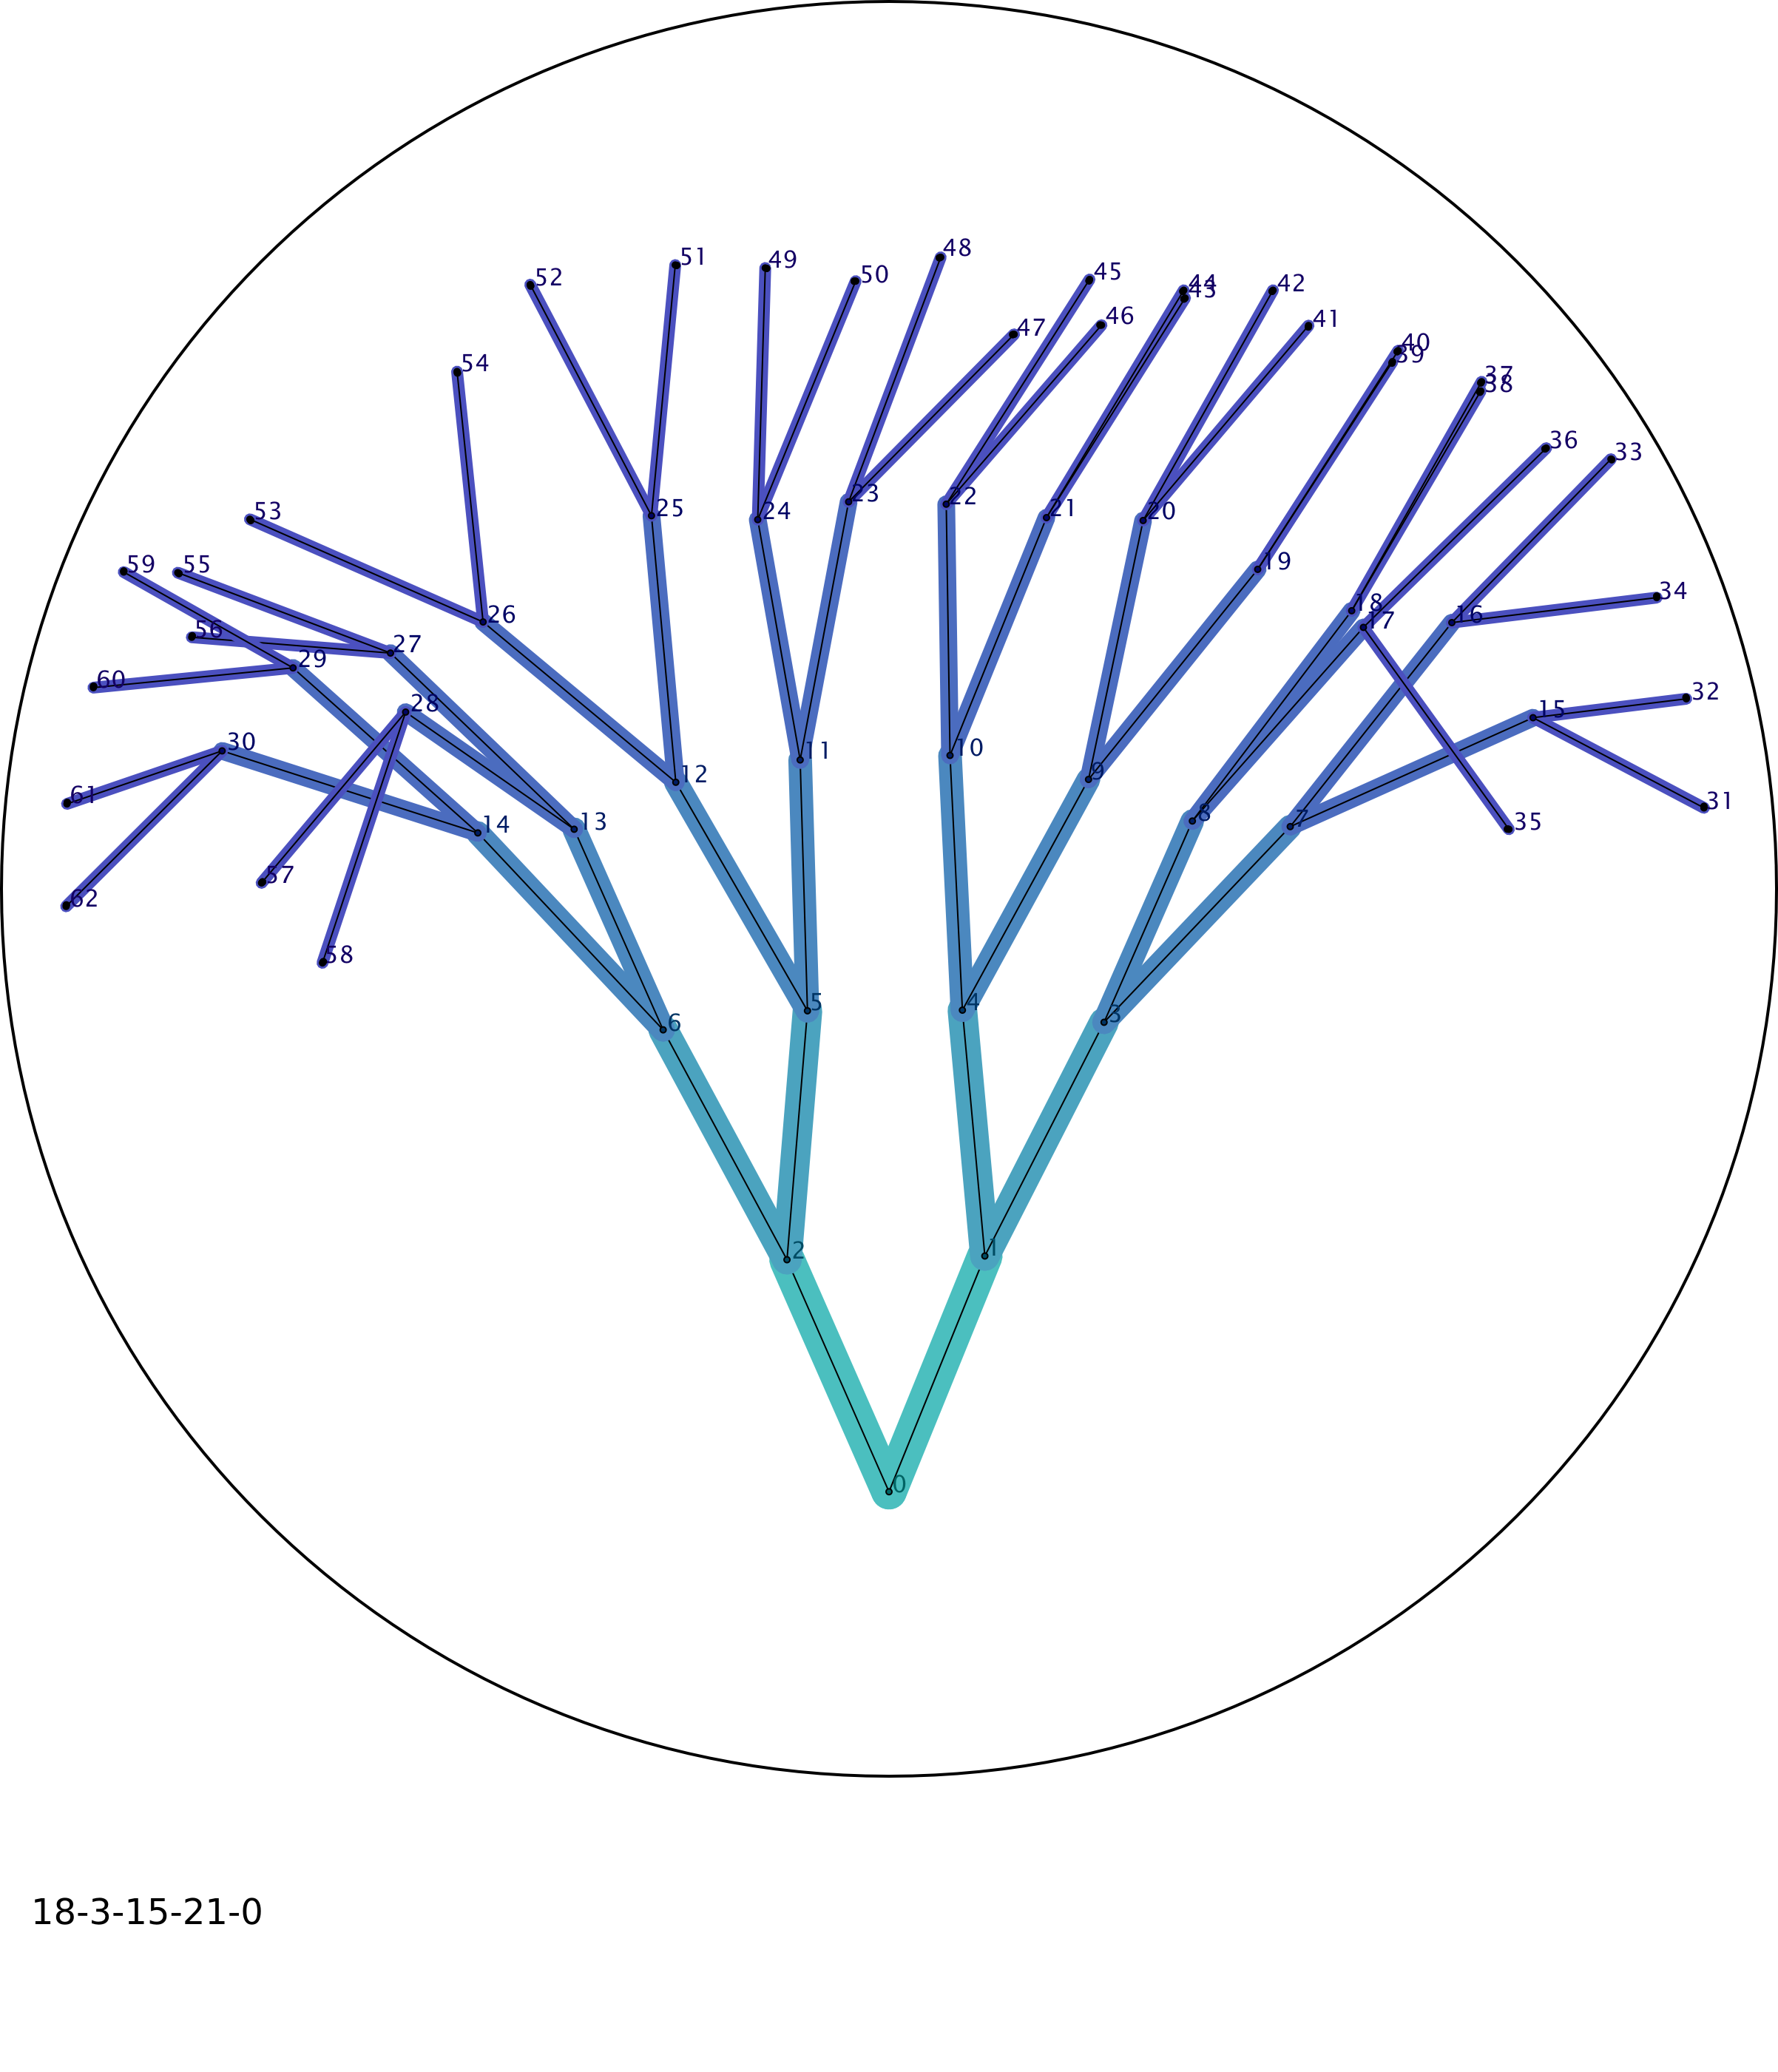
\includegraphics[width=\textwidth]{img_18-3-15-21-0}
\captionof{figure}{timetoSpawn = 3000}
\end{minipage}
\hspace{0.5cm}
\begin{minipage}[t]{\imgSize\textwidth}
\raisebox{0.175\totalheight}{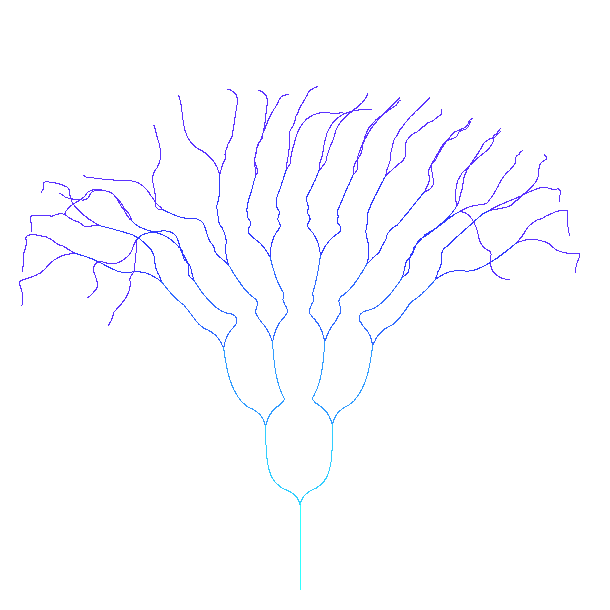
\includegraphics[width=\textwidth]{tank_timeToSpawn_trace_18-3-15-21-0_1}}
\captionof{figure}{timetoSpawn = 3000}
\end{minipage}
\vspace{0.5cm} 

%4000 
\begin{minipage}[t]{\imgSize\textwidth}
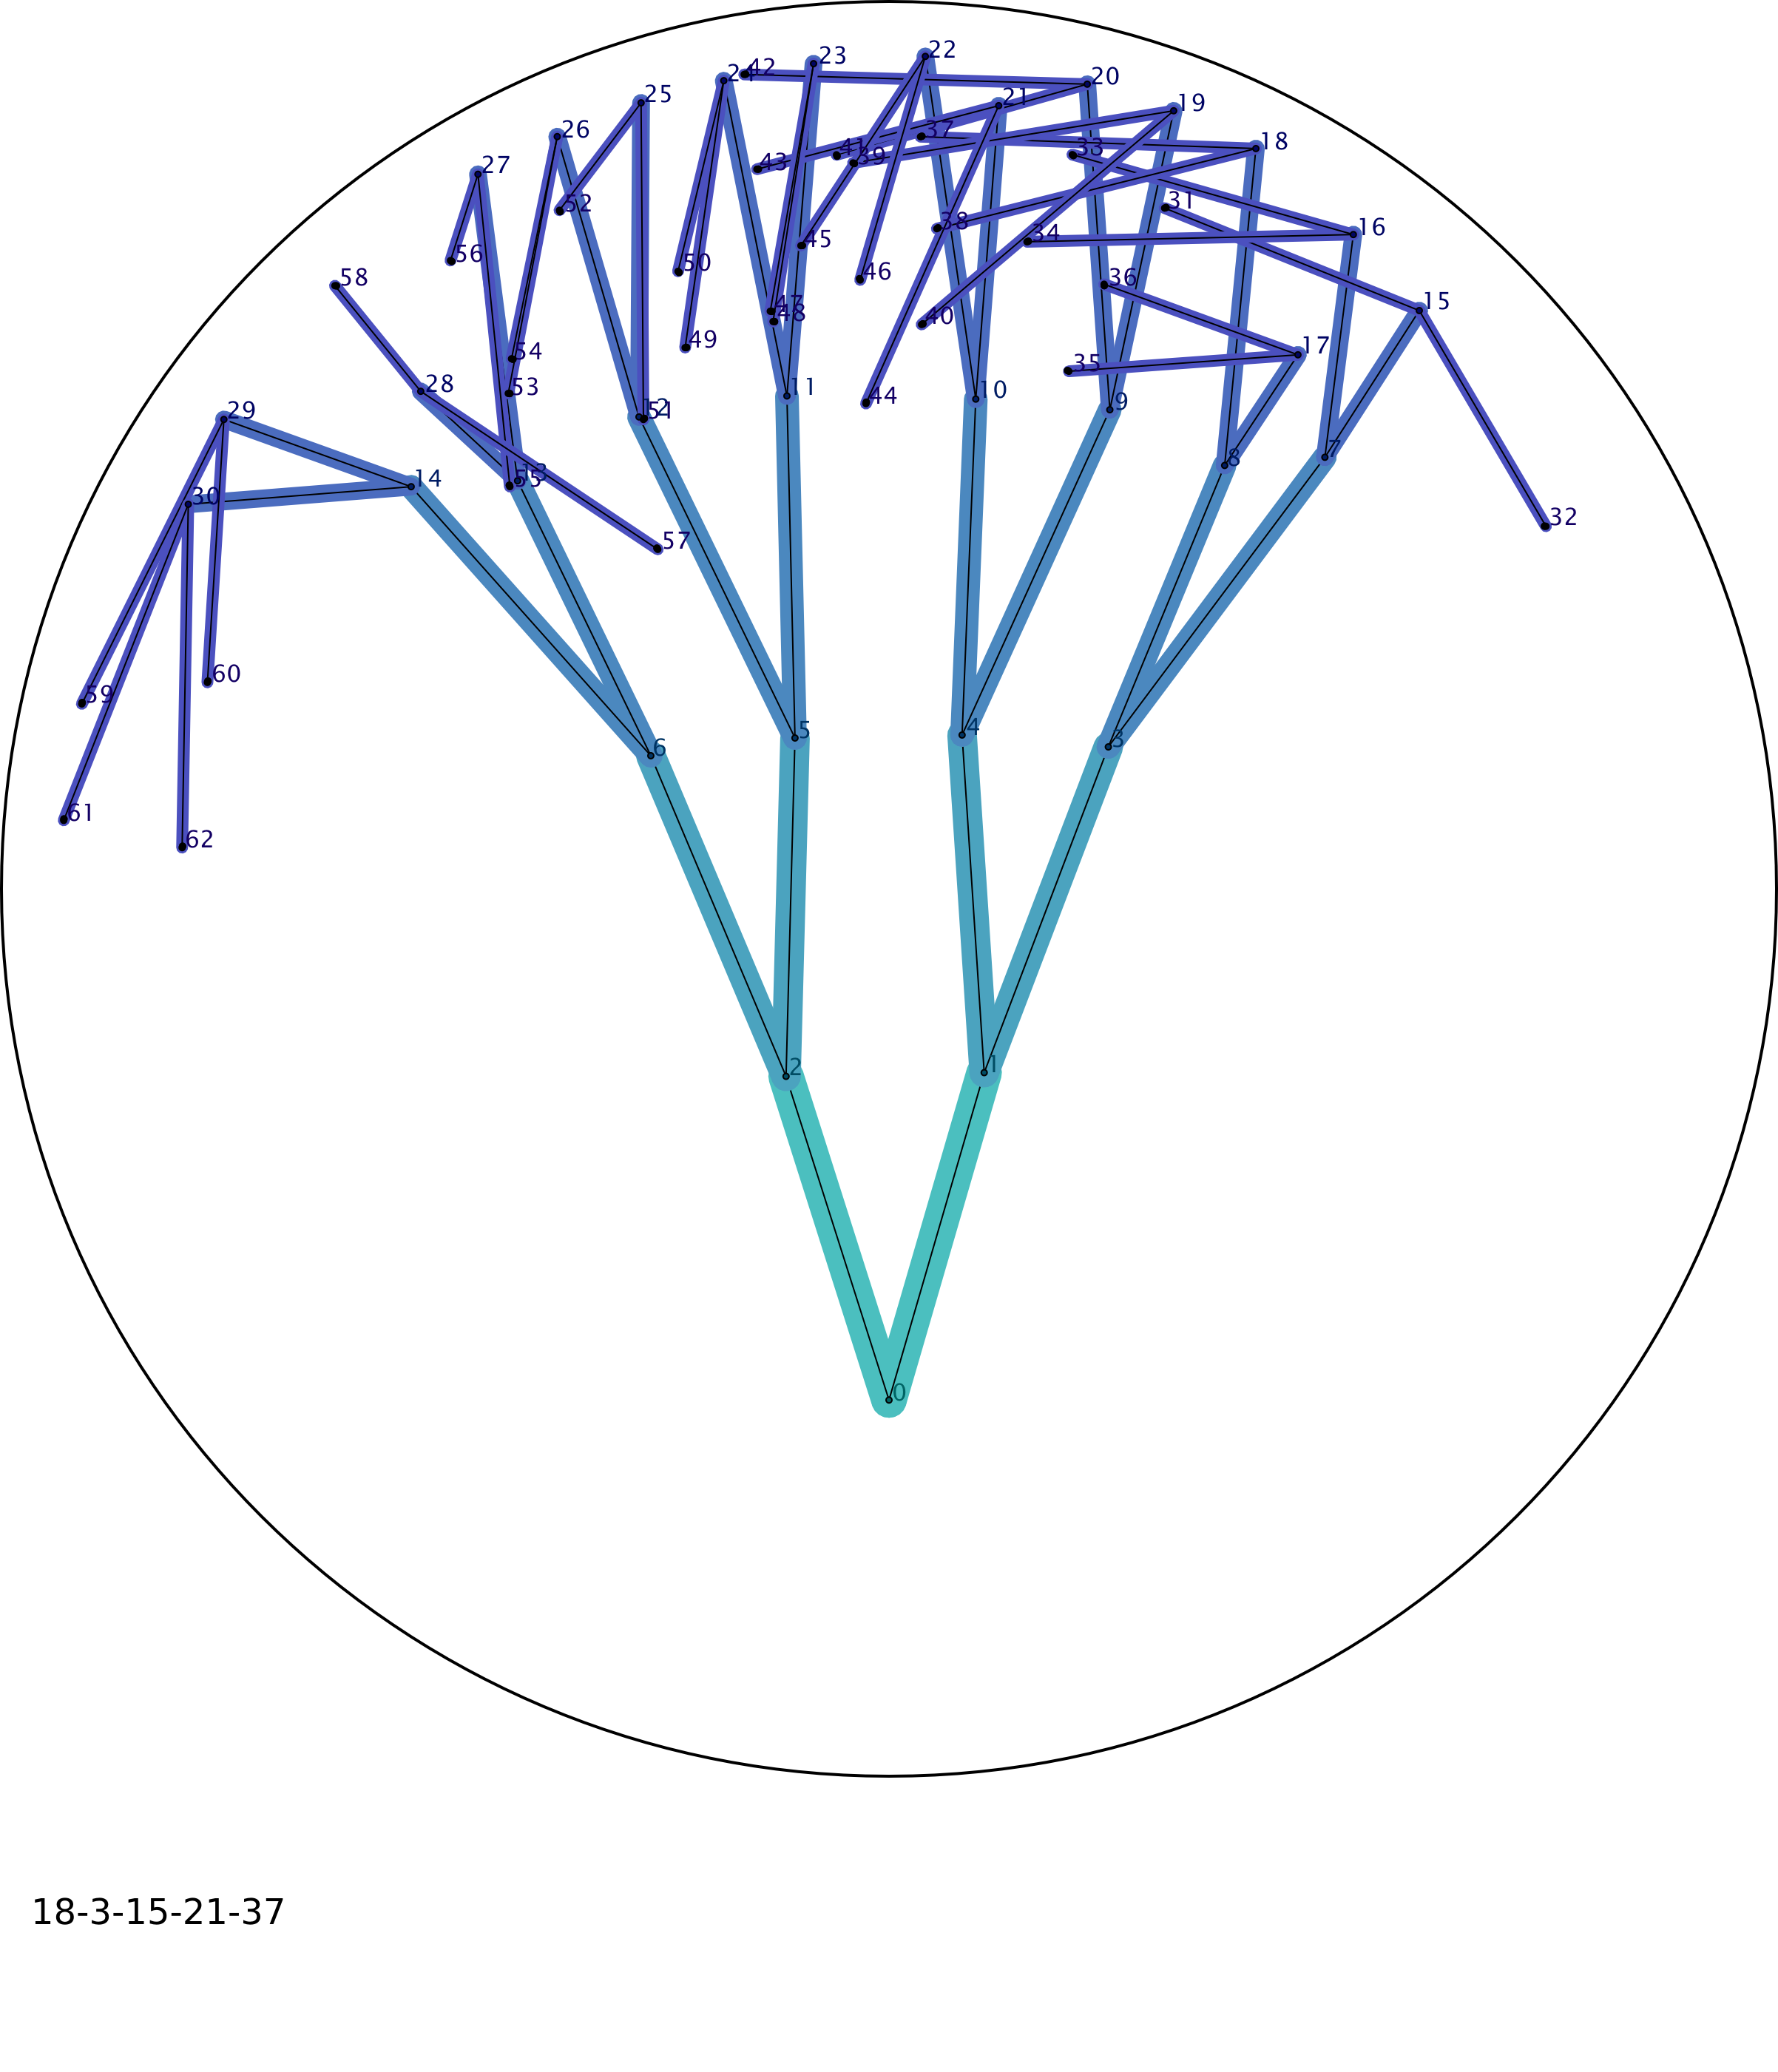
\includegraphics[width=\textwidth]{img_18-3-15-21-37}
\captionof{figure}{timetoSpawn = 4000}
\end{minipage}
\hspace{0.5cm}
\begin{minipage}[t]{\imgSize\textwidth}
\raisebox{0.175\totalheight}{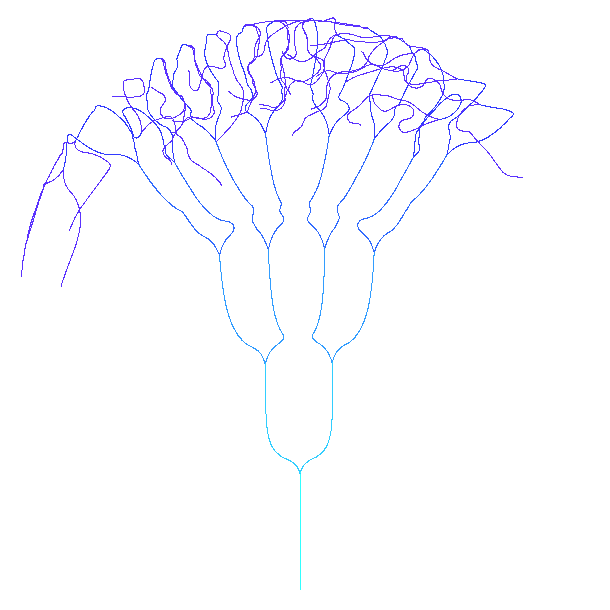
\includegraphics[width=\textwidth]{tank_timeToSpawn_trace_18-3-15-21-37_1}}
\captionof{figure}{timetoSpawn = 4000}
\end{minipage}
\vspace{0.5cm}

%5000
\begin{minipage}[t]{\imgSize\textwidth}
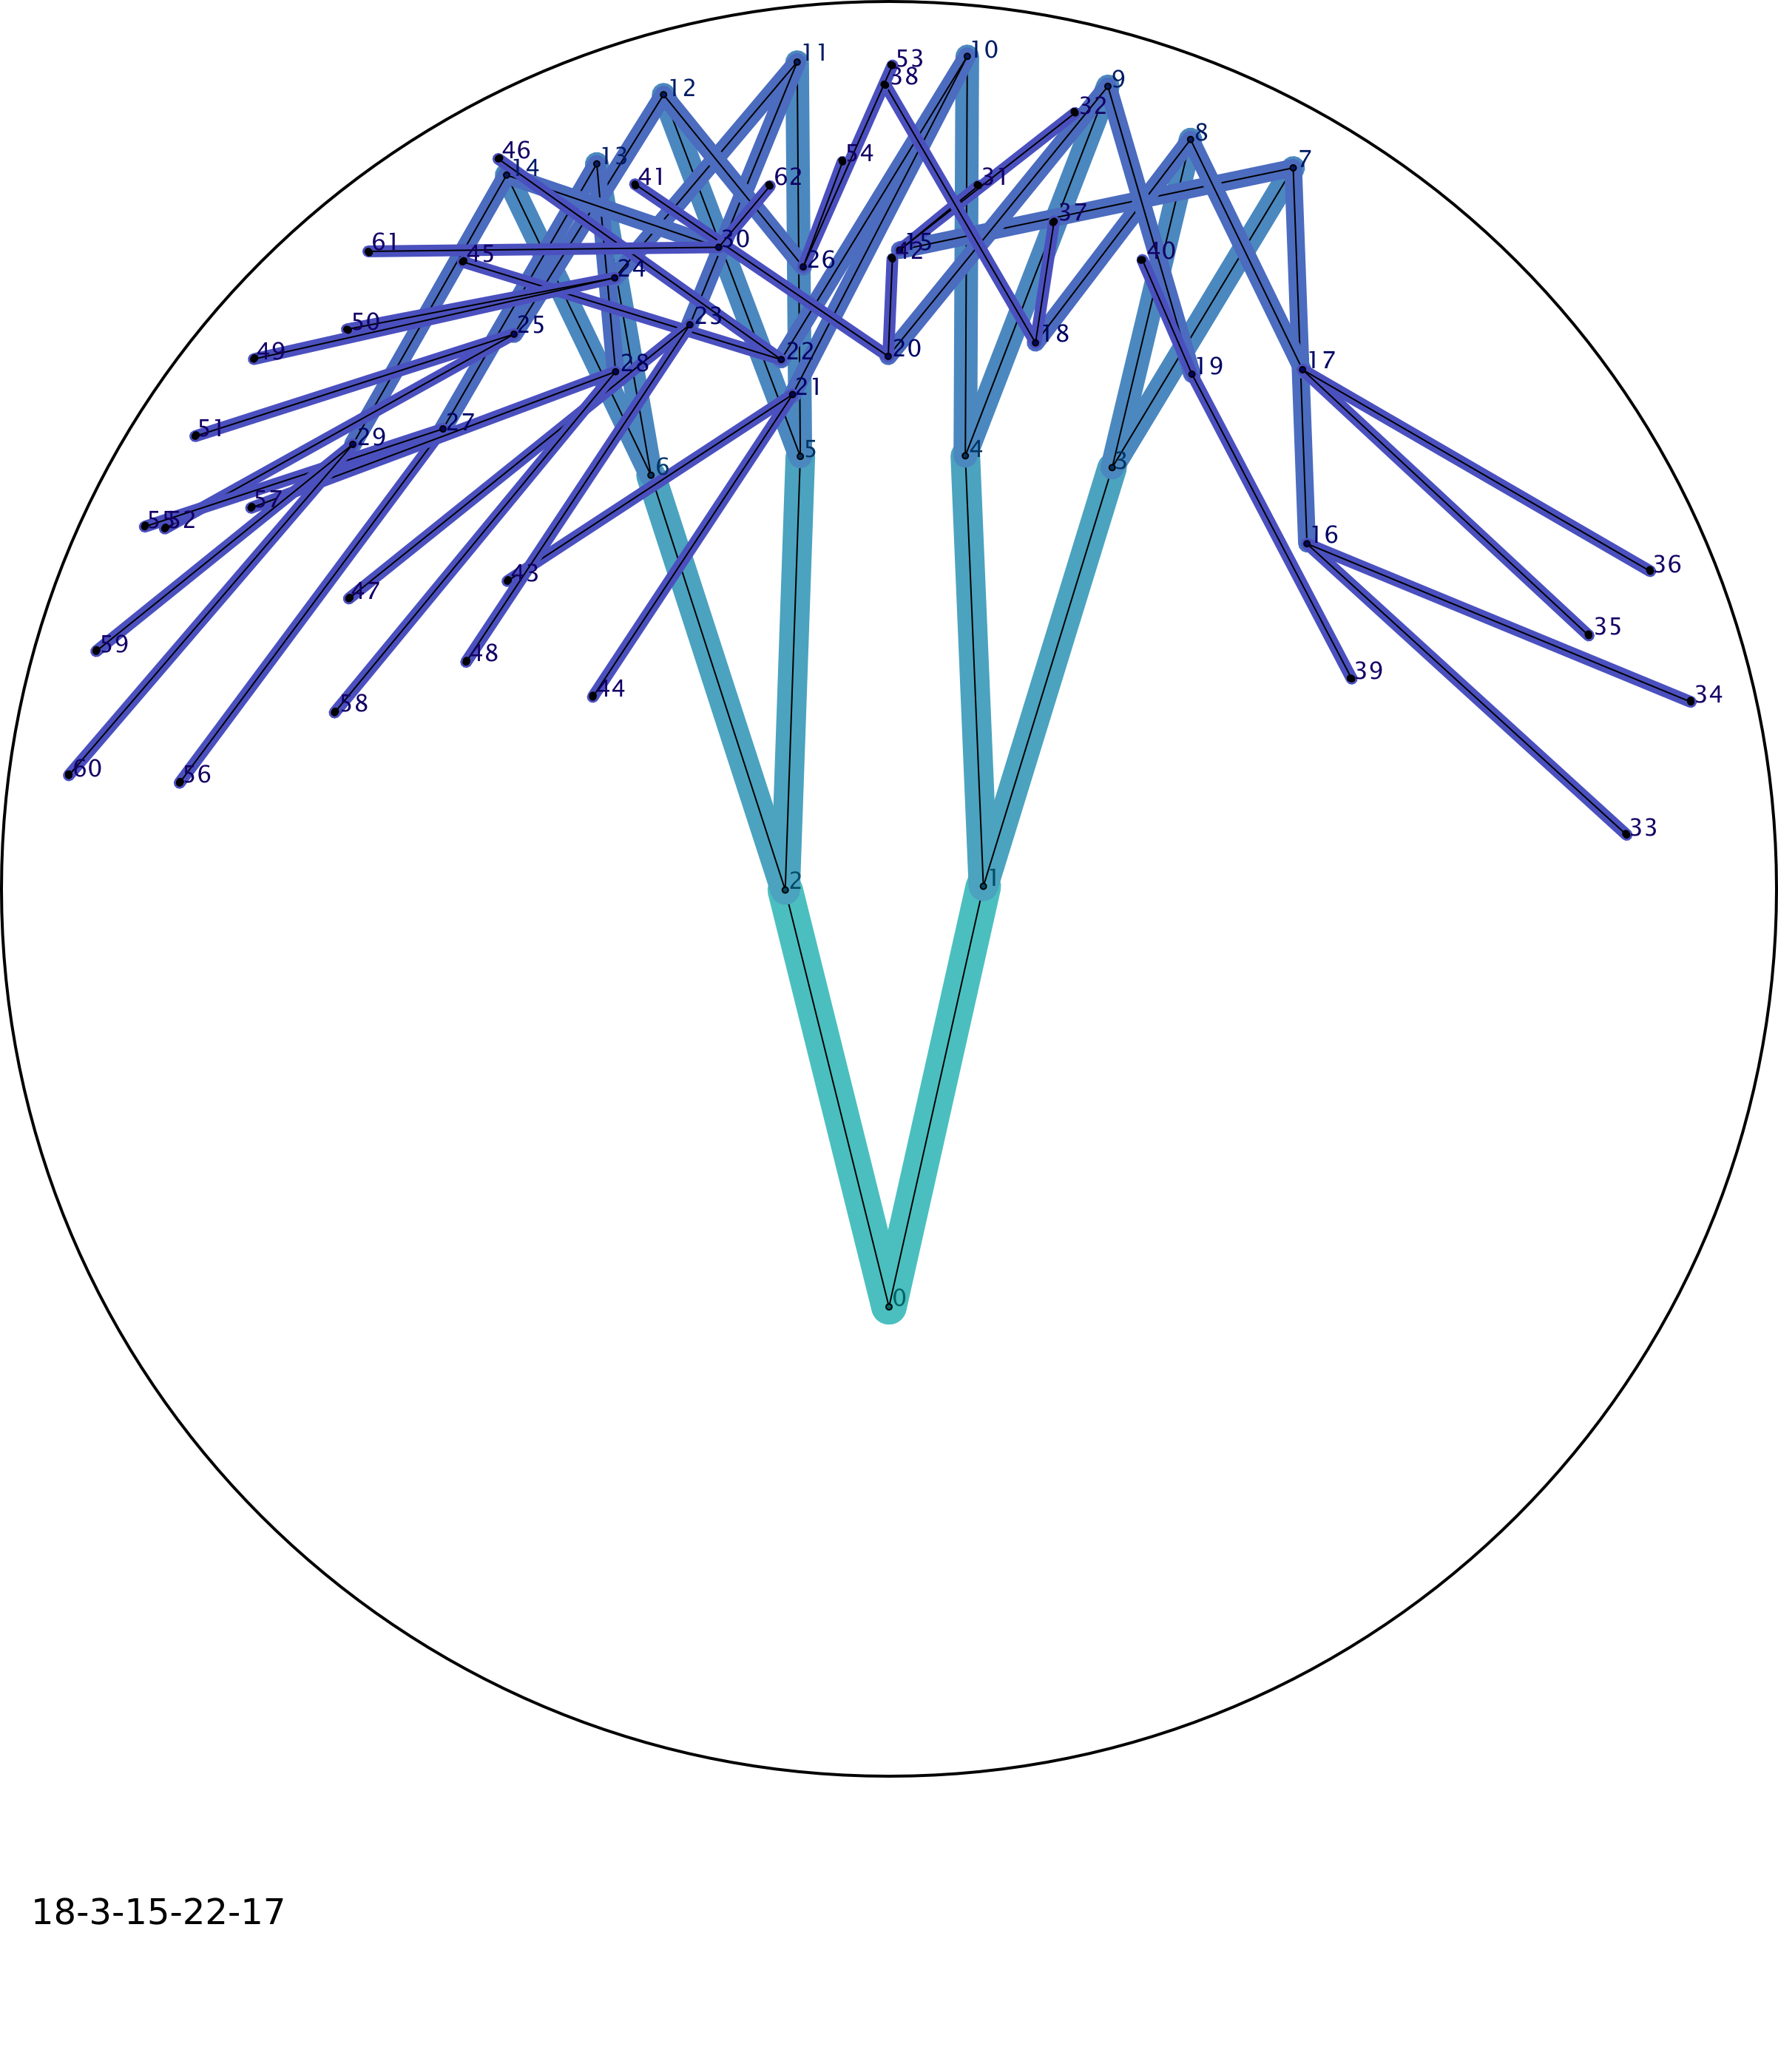
\includegraphics[width=\textwidth]{img_18-3-15-22-17}
\captionof{figure}{timetoSpawn = 5000}
\end{minipage}
\hspace{0.5cm}
\begin{minipage}[t]{\imgSize\textwidth}
\raisebox{0.175\totalheight}{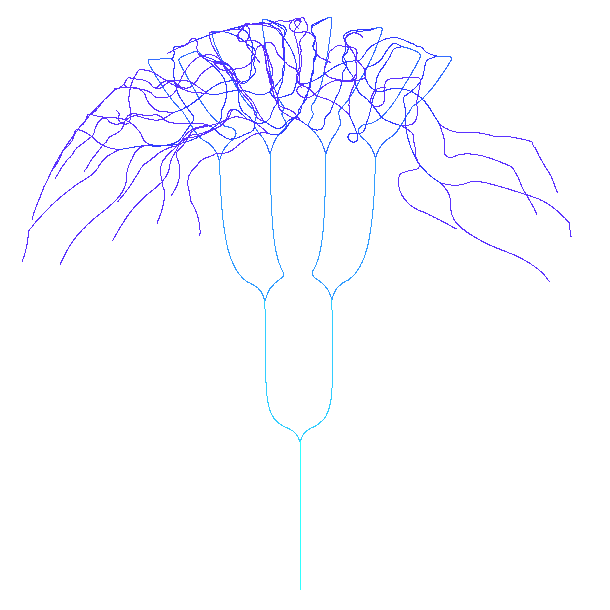
\includegraphics[width=\textwidth]{tank_timeToSpawn_trace_18-3-15-22-17_1}}
\captionof{figure}{timetoSpawn = 5000}
\end{minipage}
\vspace{0.5cm} 

%6000  def
\begin{minipage}[t]{\imgSize\textwidth}
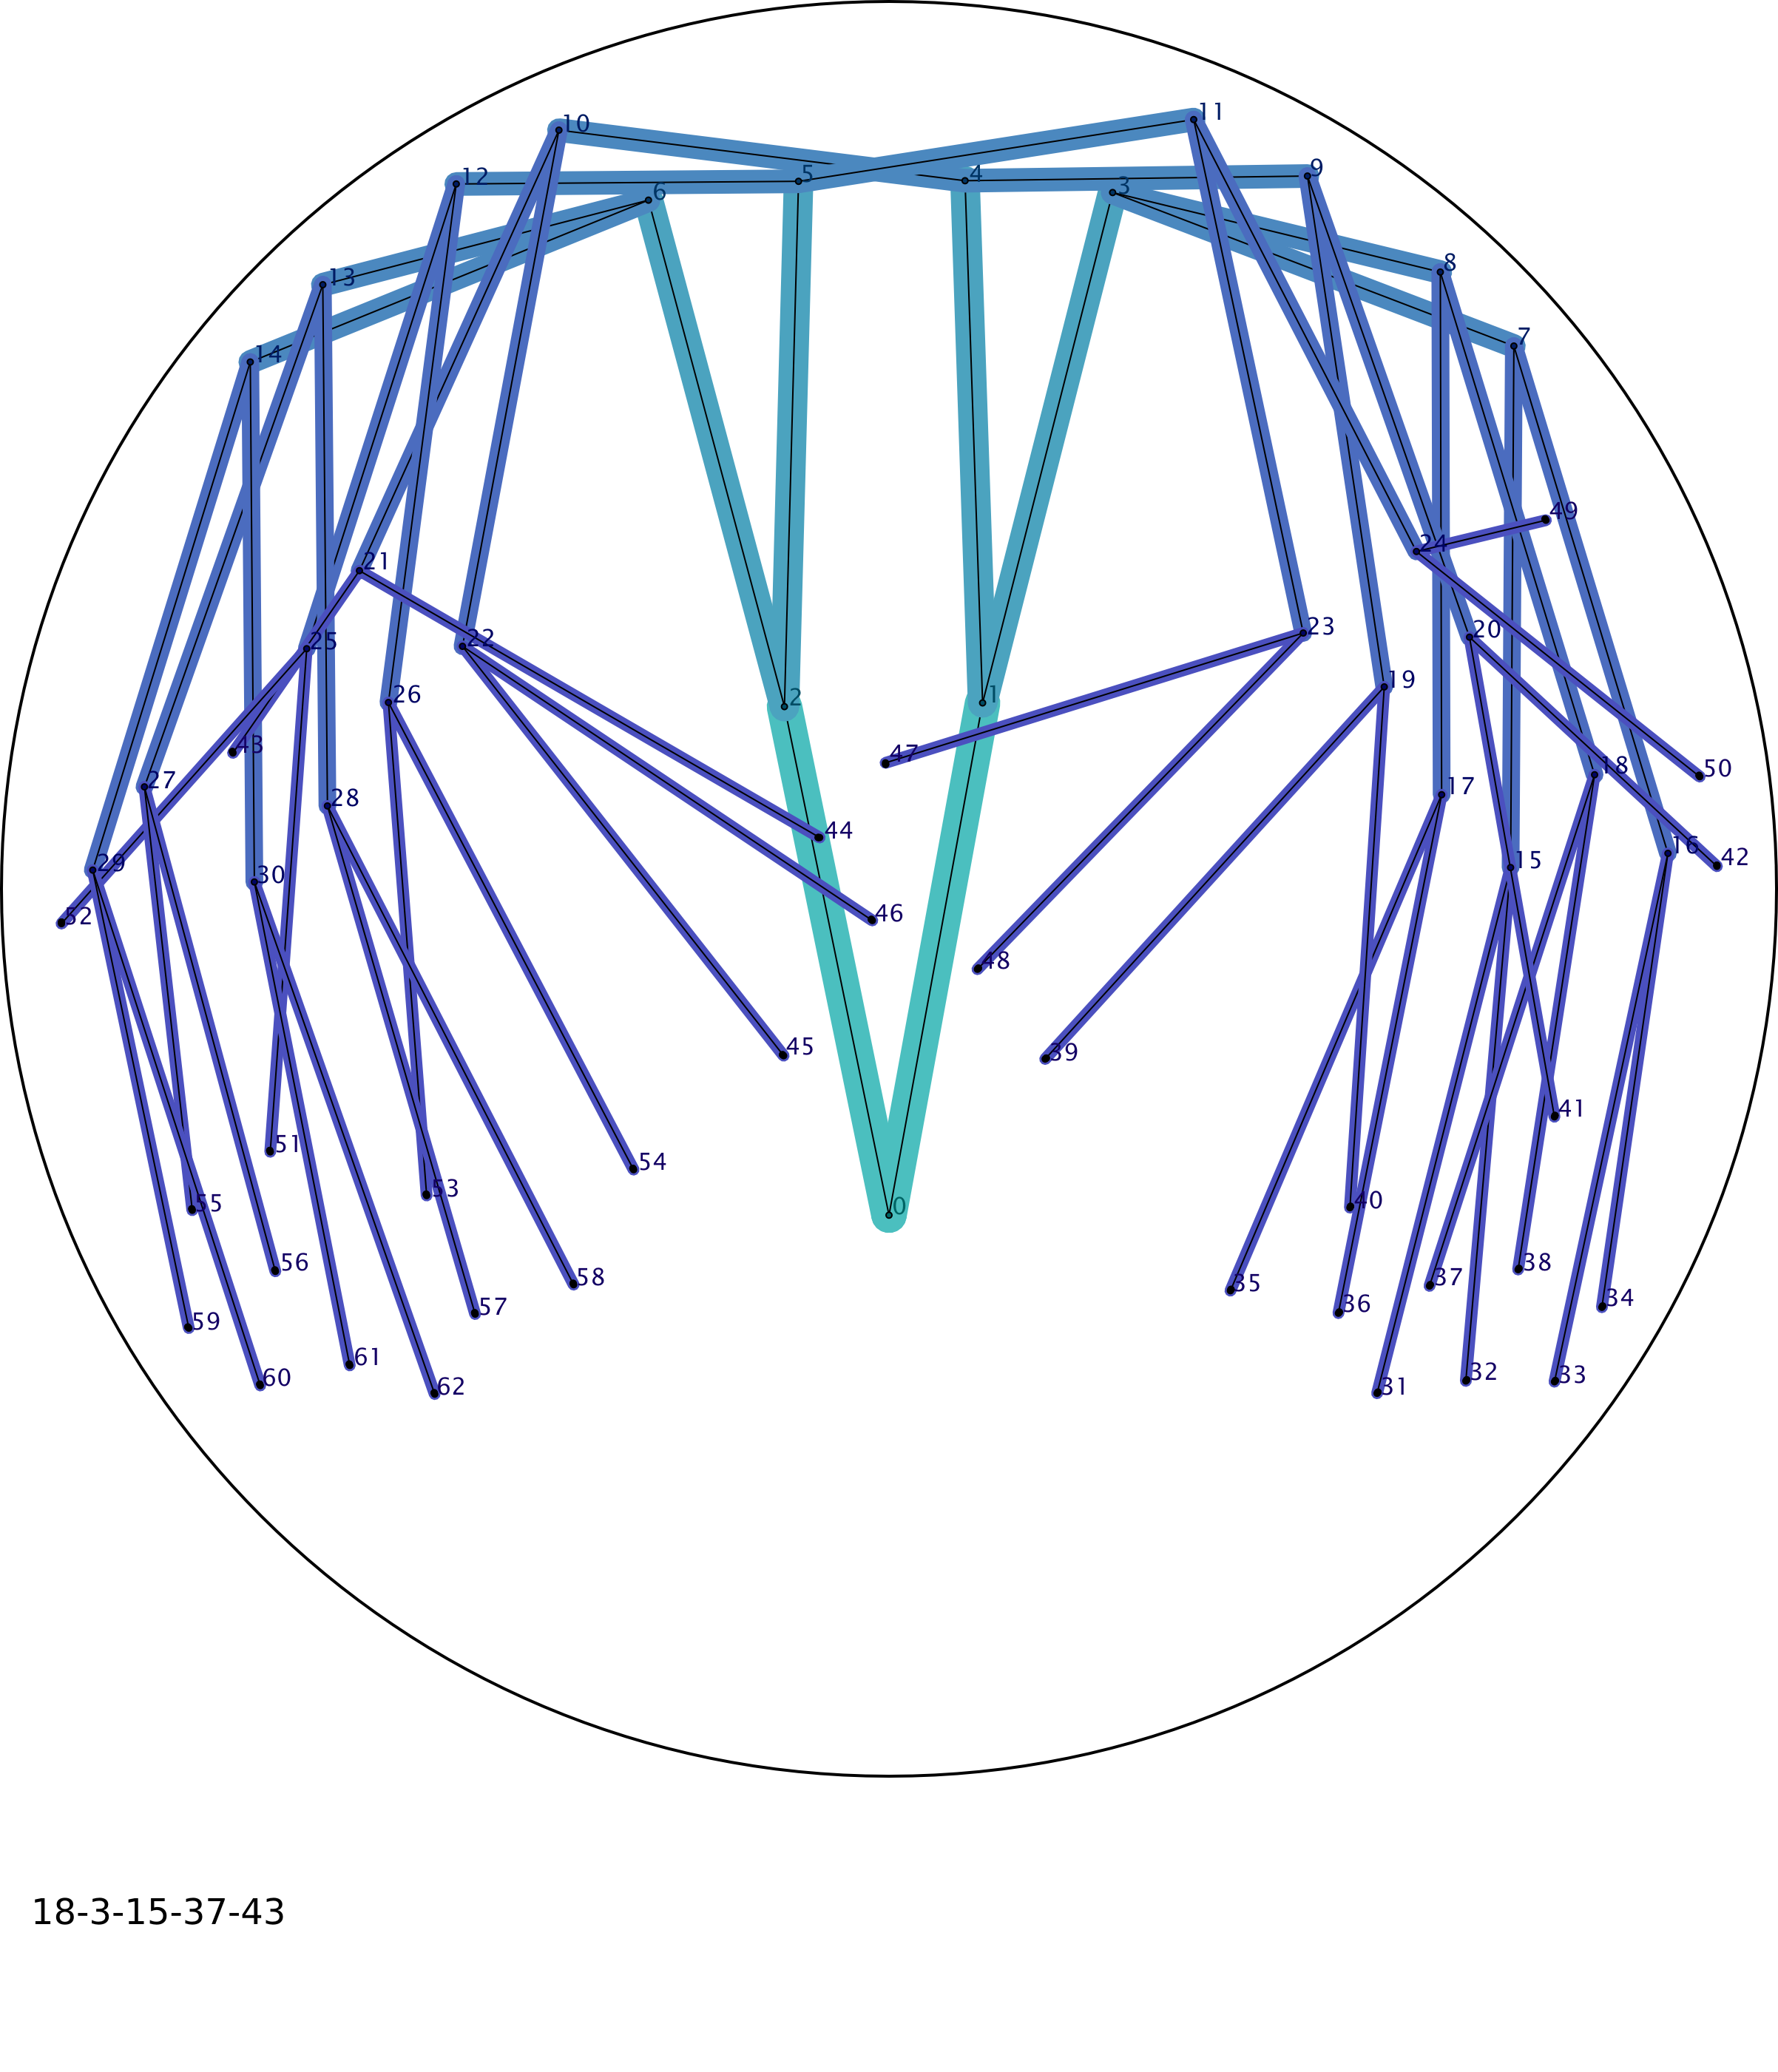
\includegraphics[width=\textwidth]{img_18-3-15-37-43}
\captionof{figure}{timetoSpawn = 6000 (default)}
\end{minipage}
\hspace{0.5cm}
\begin{minipage}[t]{\imgSize\textwidth}
\raisebox{0.175\totalheight}{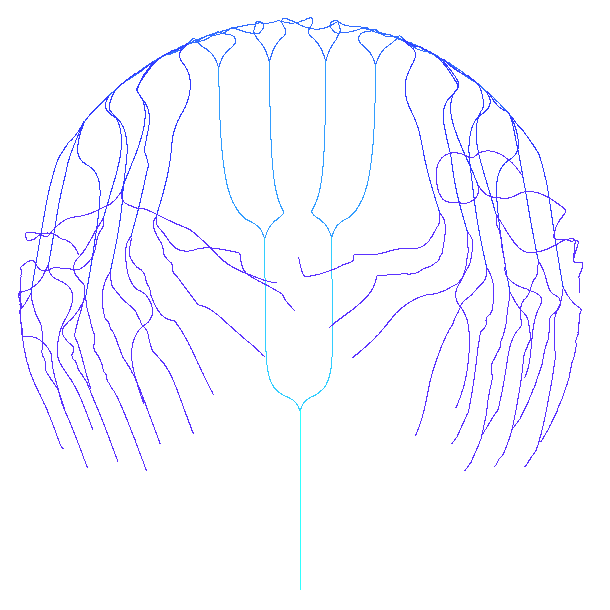
\includegraphics[width=\textwidth]{tank_default_trace_18-3-15-37-43_1}}
\captionof{figure}{timetoSpawn = 6000 (default)}
\end{minipage}
\vspace{0.5cm}

%8000
\begin{minipage}[t]{\imgSize\textwidth}
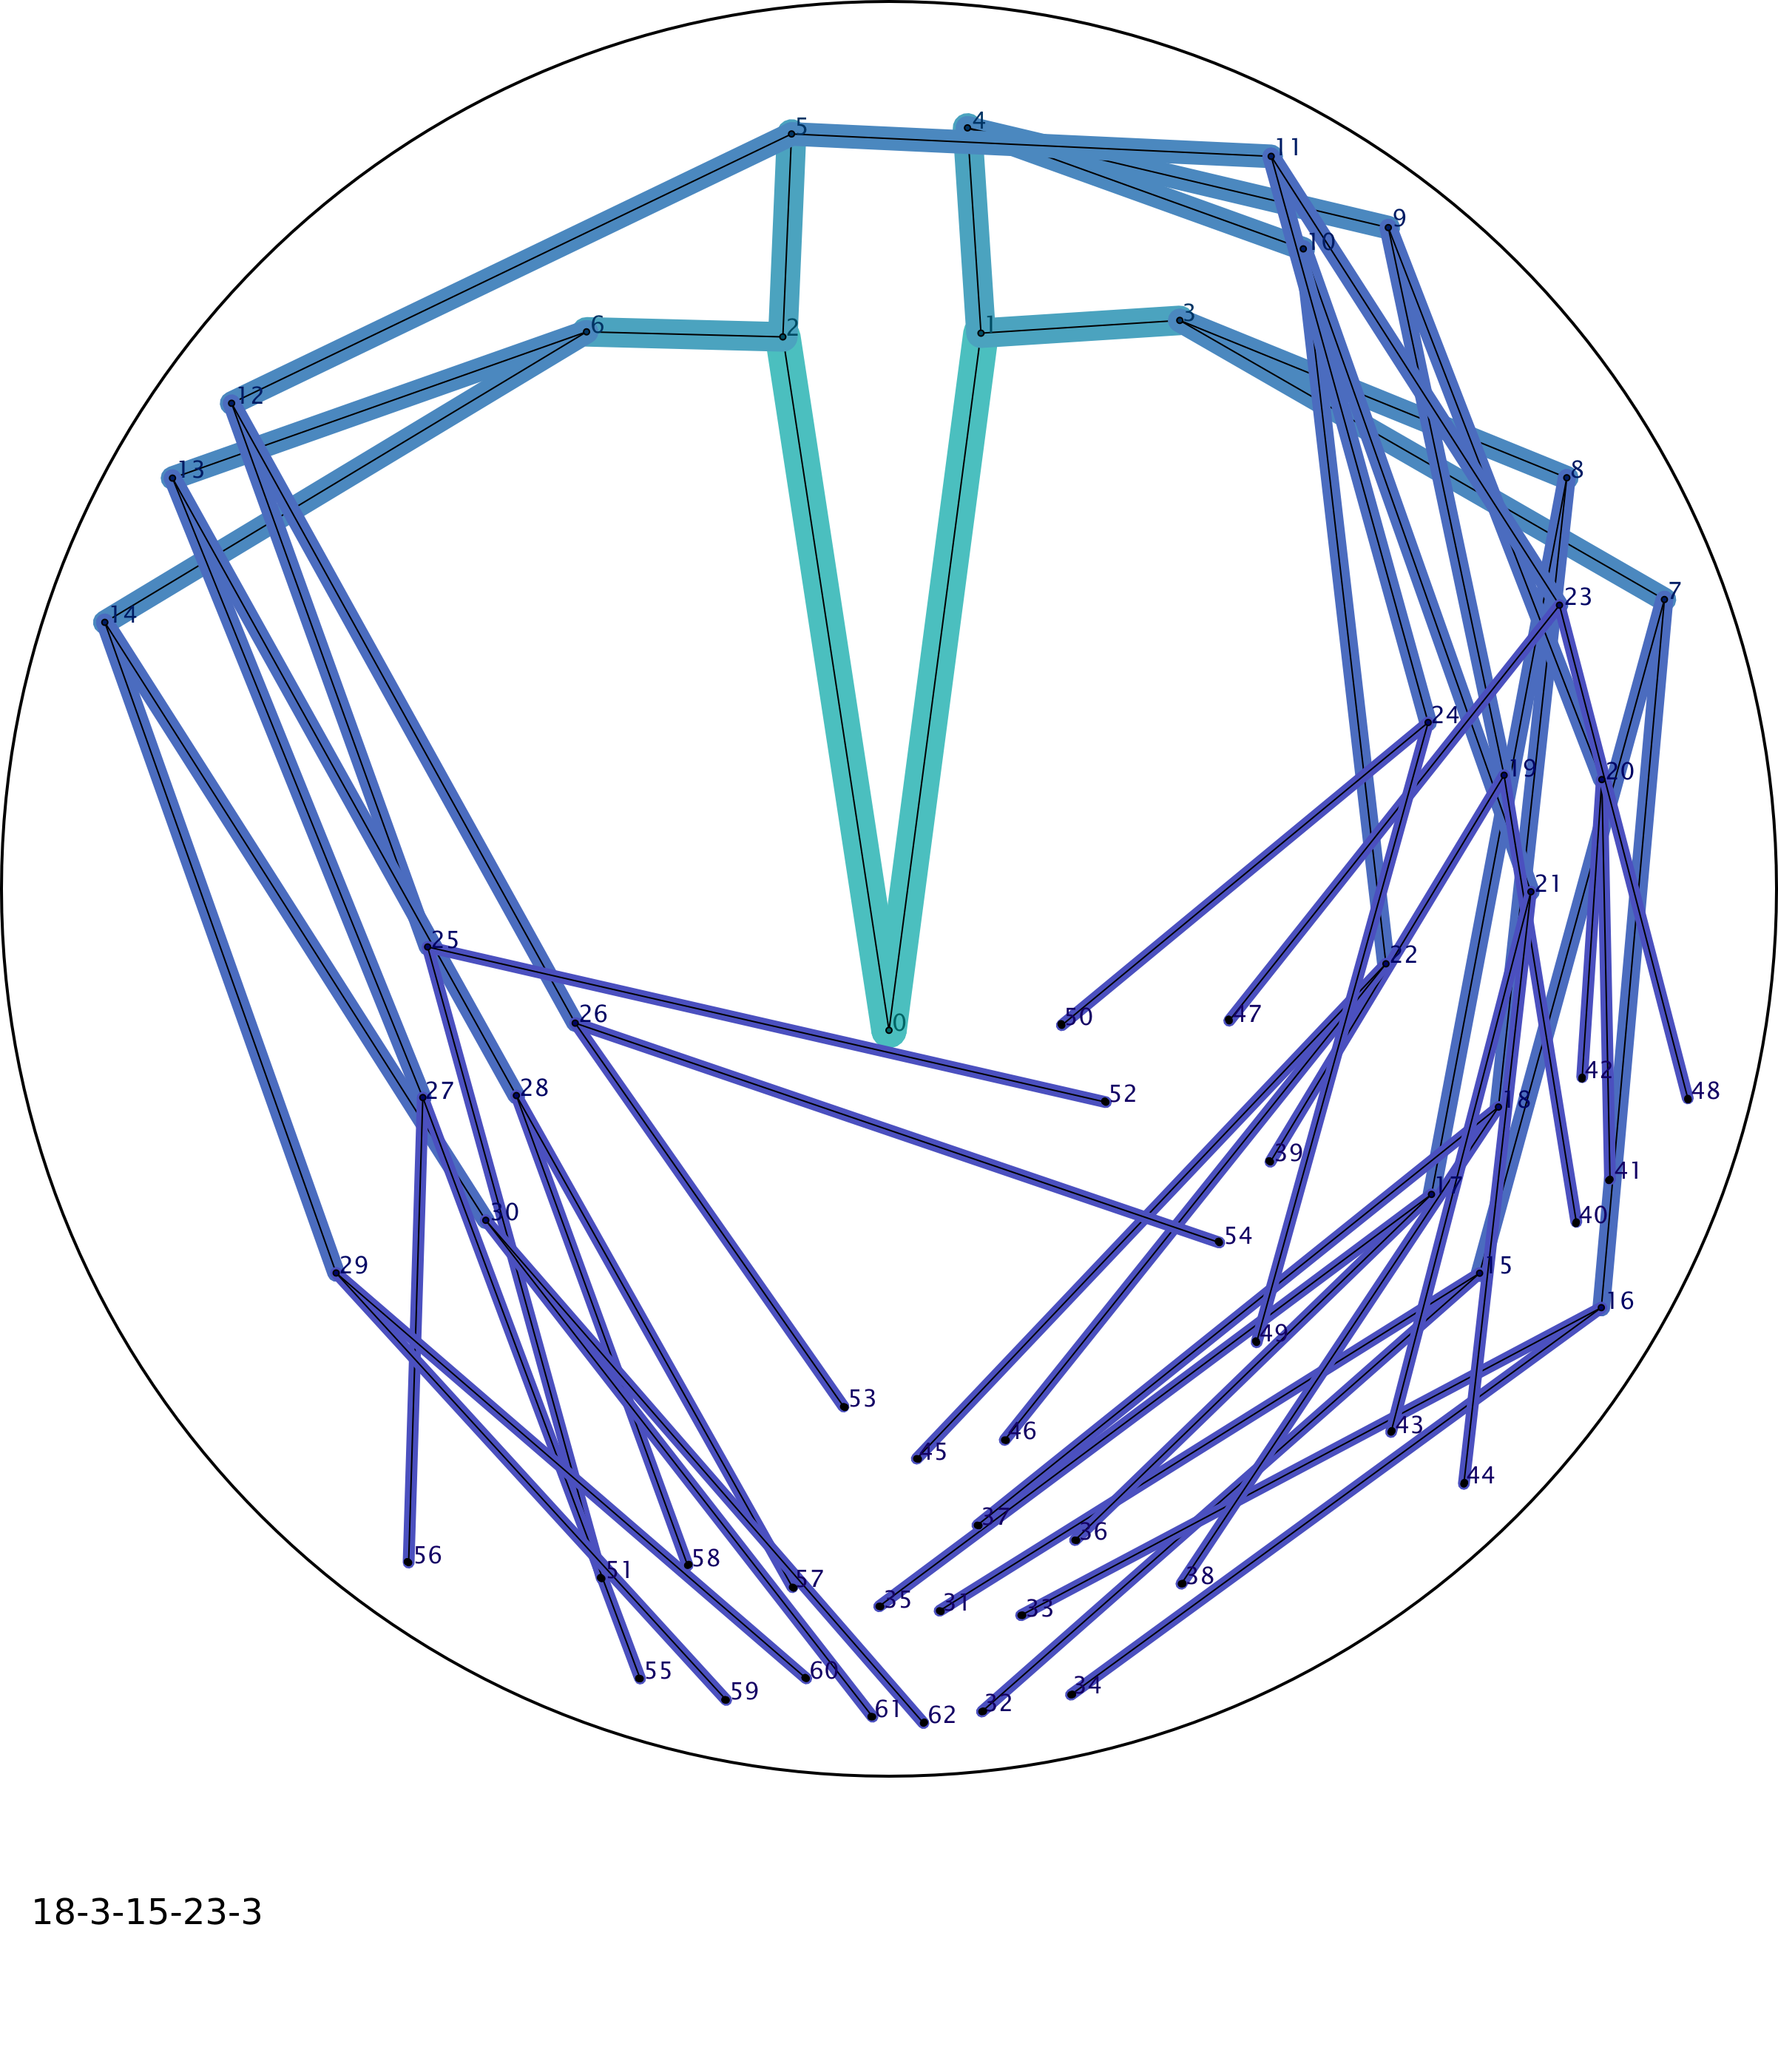
\includegraphics[width=\textwidth]{img_18-3-15-23-3}
\captionof{figure}{timetoSpawn = 8000}
\end{minipage}
\hspace{0.5cm}
\begin{minipage}[t]{\imgSize\textwidth}
\raisebox{0.175\totalheight}{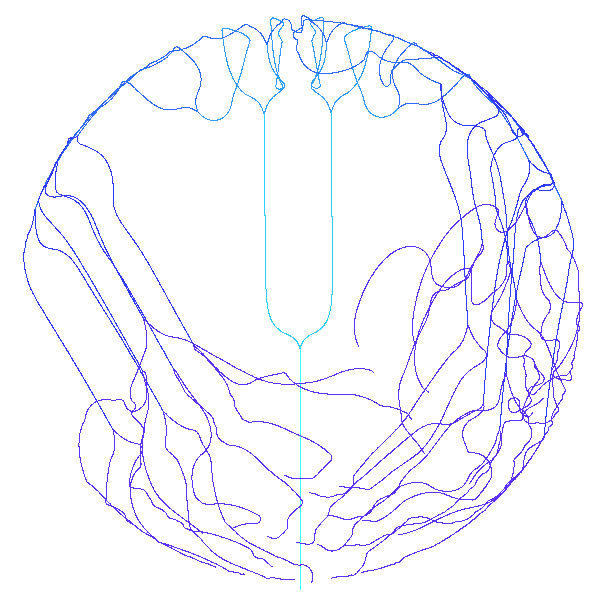
\includegraphics[width=\textwidth]{tank_timeToSpawn_trace_18-3-15-23-3_1}}
\captionof{figure}{timetoSpawn = 8000}
\end{minipage}
\vspace{0.5cm}

\newpage
\subsubsection{Variations of "spawnAnglesDegree"}
%0
\begin{minipage}[t]{\imgSize\textwidth}
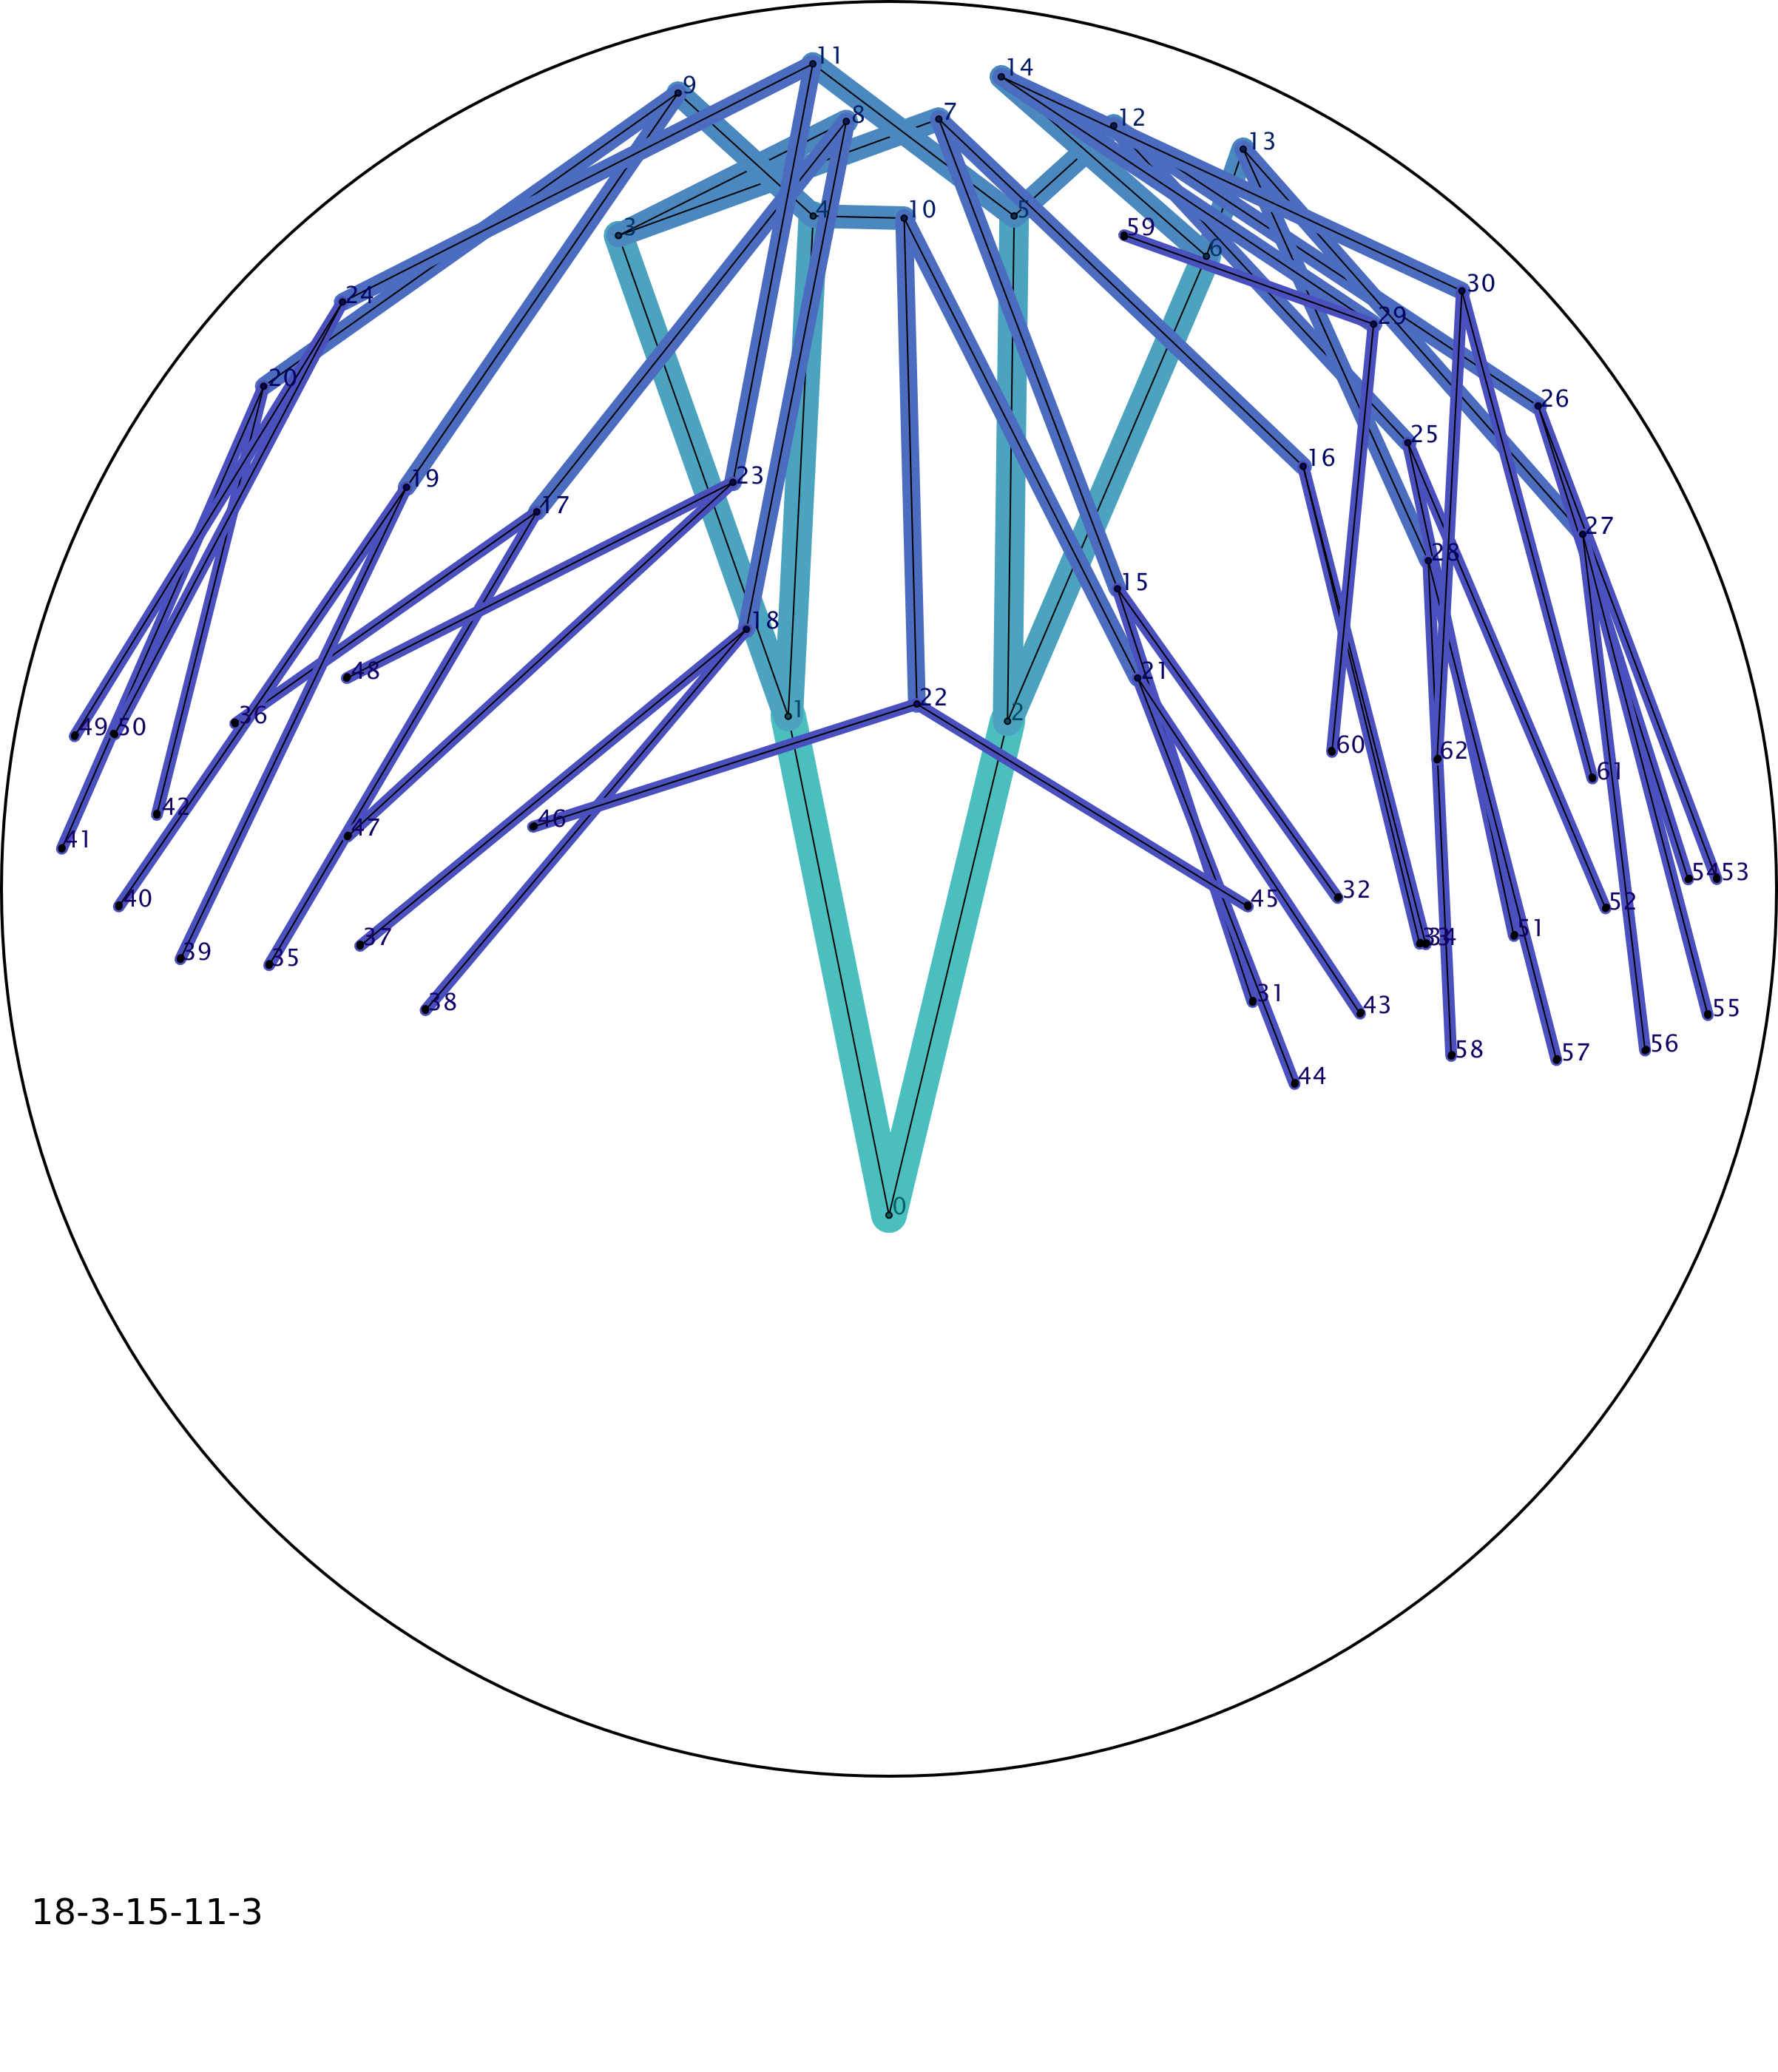
\includegraphics[width=\textwidth]{img_18-3-15-11-3}
\captionof{figure}{spawnAnglesDegree = +/-0}
\end{minipage}
\hspace{0.5cm}
\begin{minipage}[t]{\imgSize\textwidth}
\raisebox{0.175\totalheight}{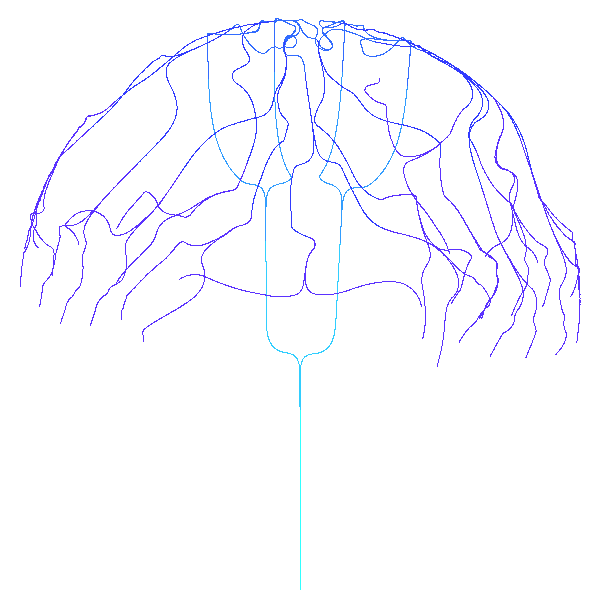
\includegraphics[width=\textwidth]{tank_spawnAnglesDegree_trace_18-3-15-11-3_1}}
\captionof{figure}{spawnAnglesDegree = +/-0}
\end{minipage}
\vspace{0.5cm} 

%20
\begin{minipage}[t]{\imgSize\textwidth}
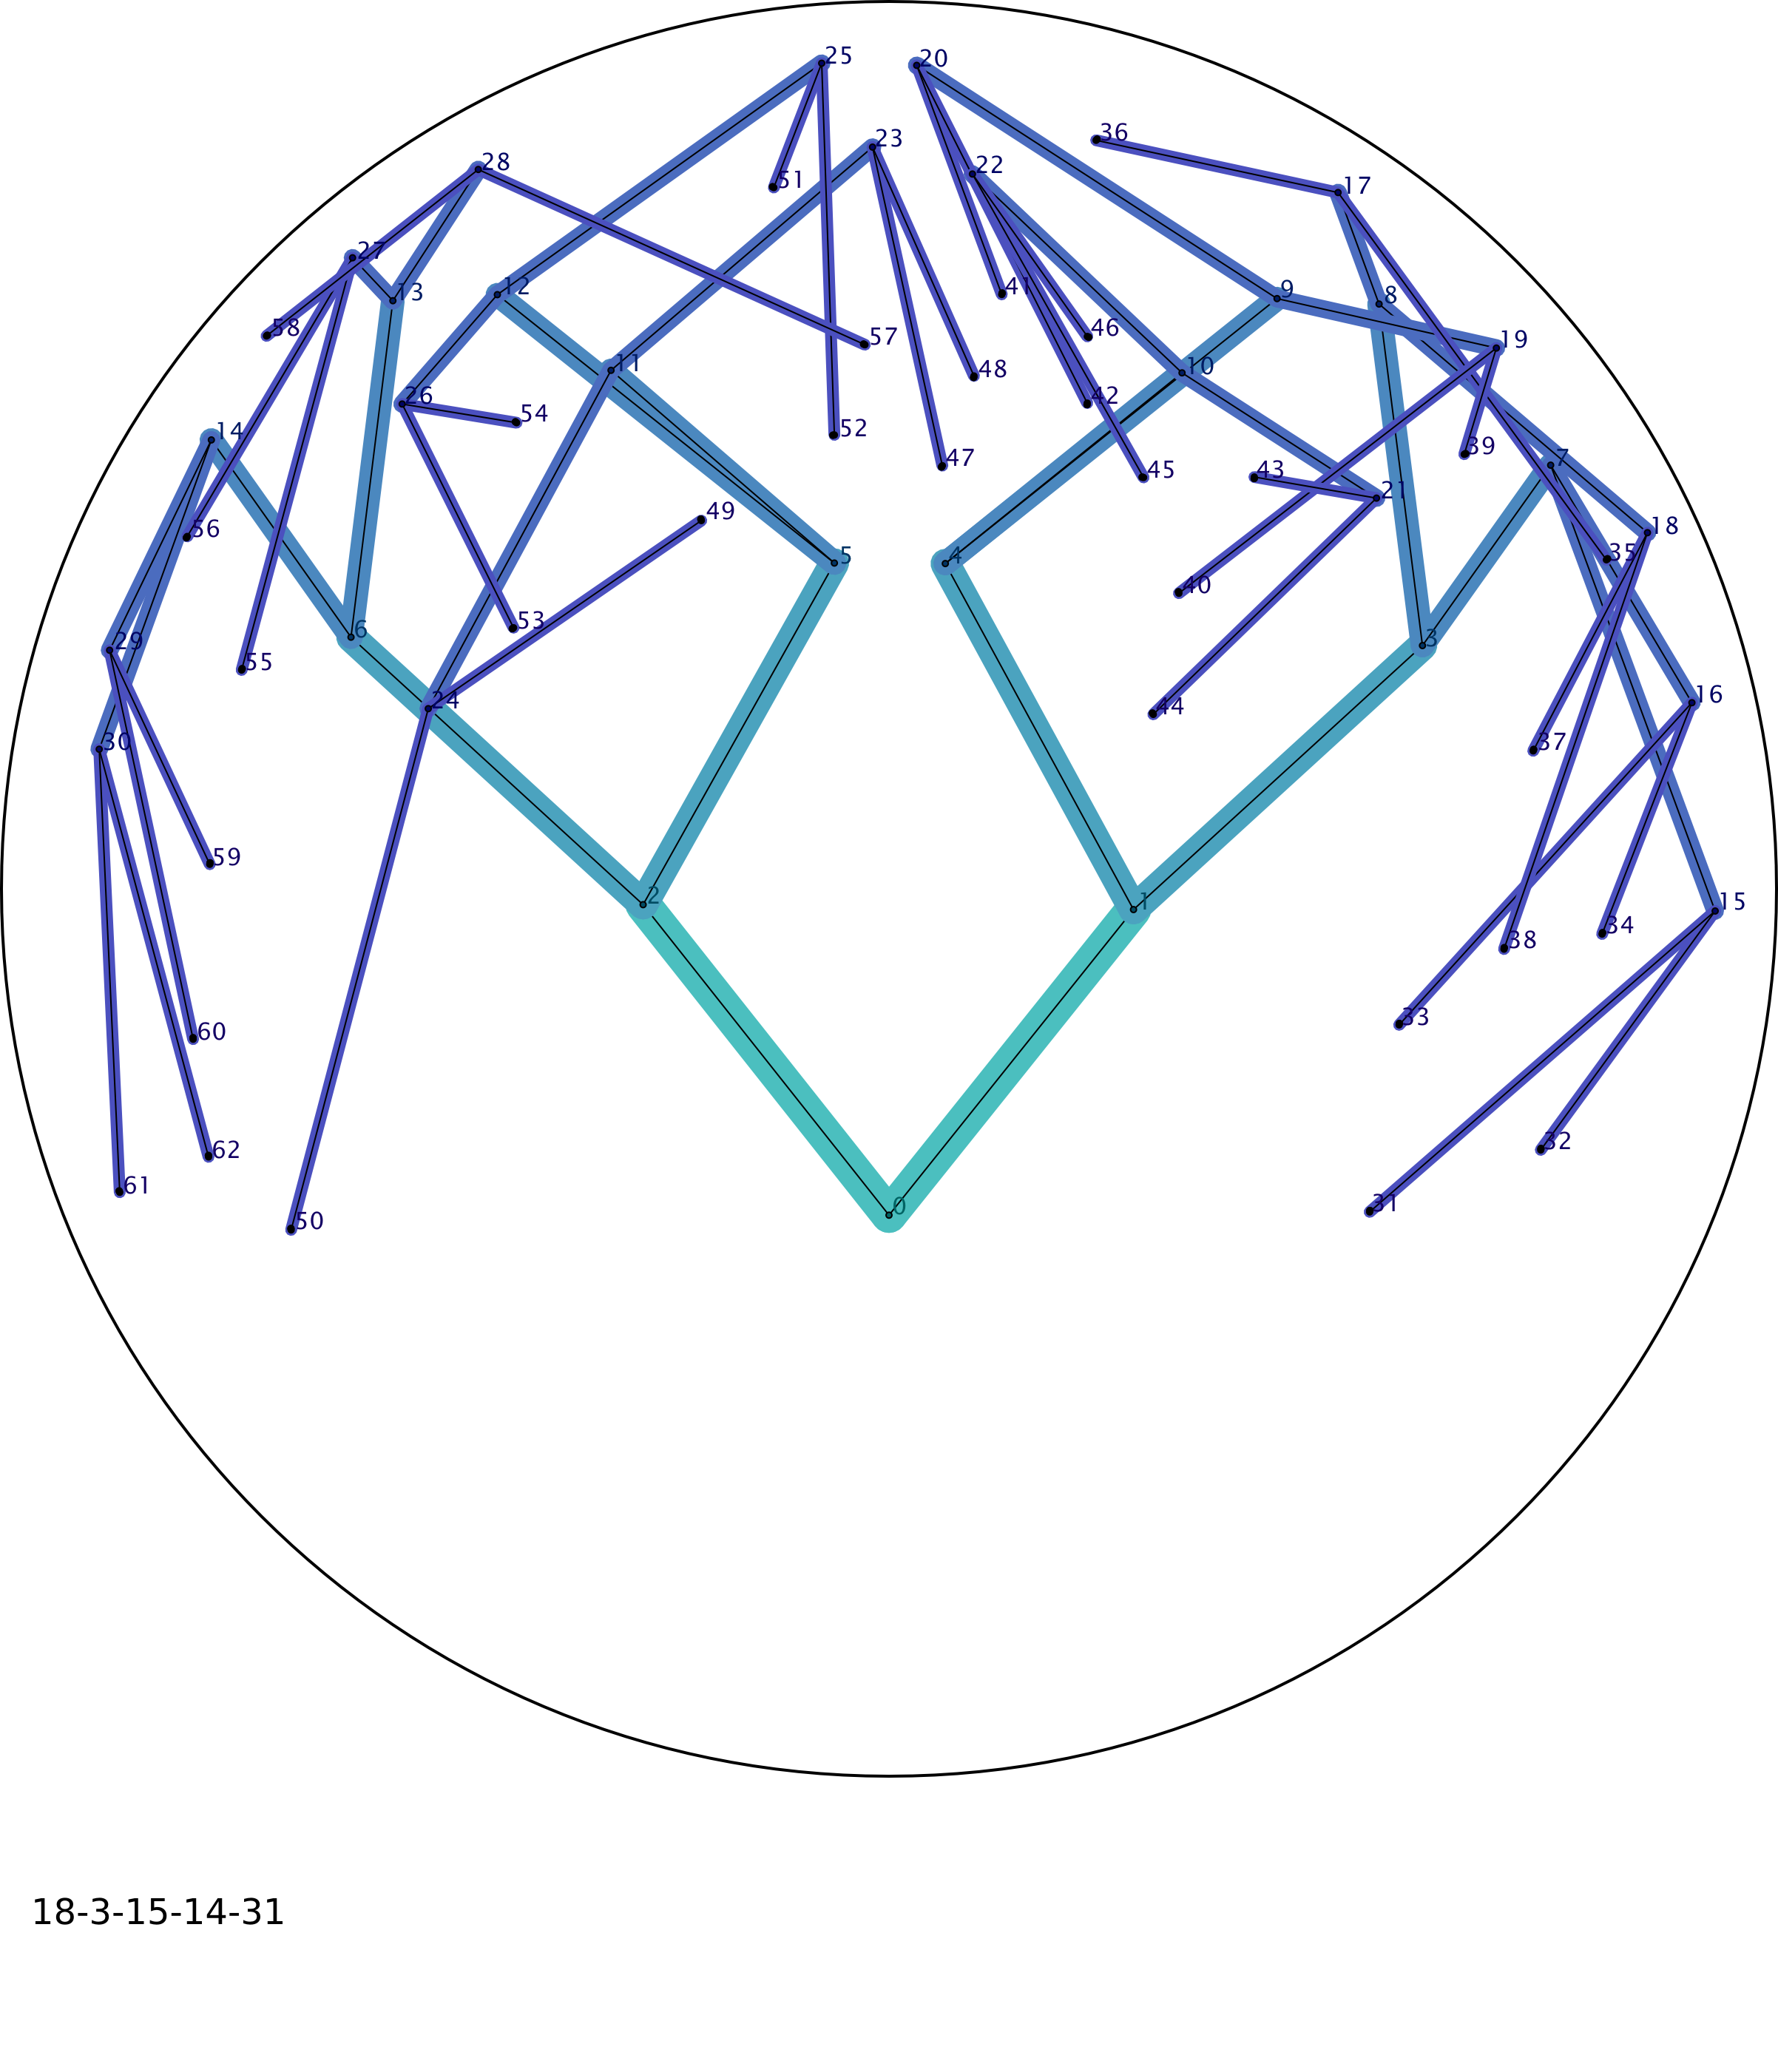
\includegraphics[width=\textwidth]{img_18-3-15-14-31}
\captionof{figure}{spawnAnglesDegree = +/-20}
\end{minipage}
\hspace{0.5cm}
\begin{minipage}[t]{\imgSize\textwidth}
\raisebox{0.175\totalheight}{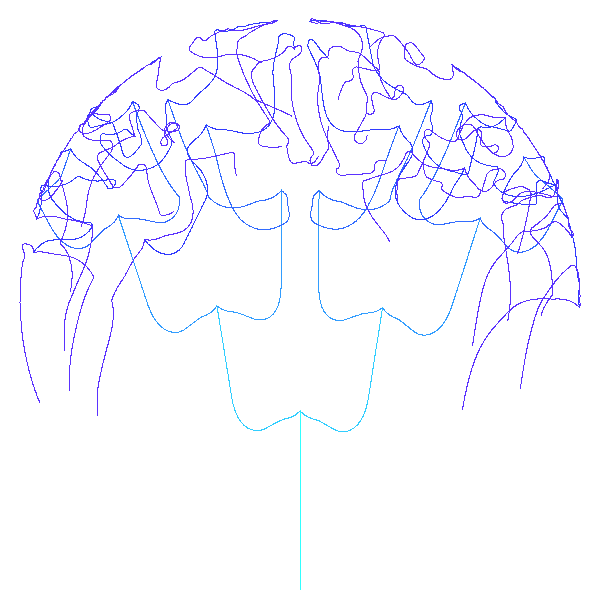
\includegraphics[width=\textwidth]{tank_spawnAnglesDegree_trace_18-3-15-14-31_1}}
\captionof{figure}{spawnAnglesDegree = +/-20}
\end{minipage}
\vspace{0.5cm} 

%45
\begin{minipage}[t]{\imgSize\textwidth}
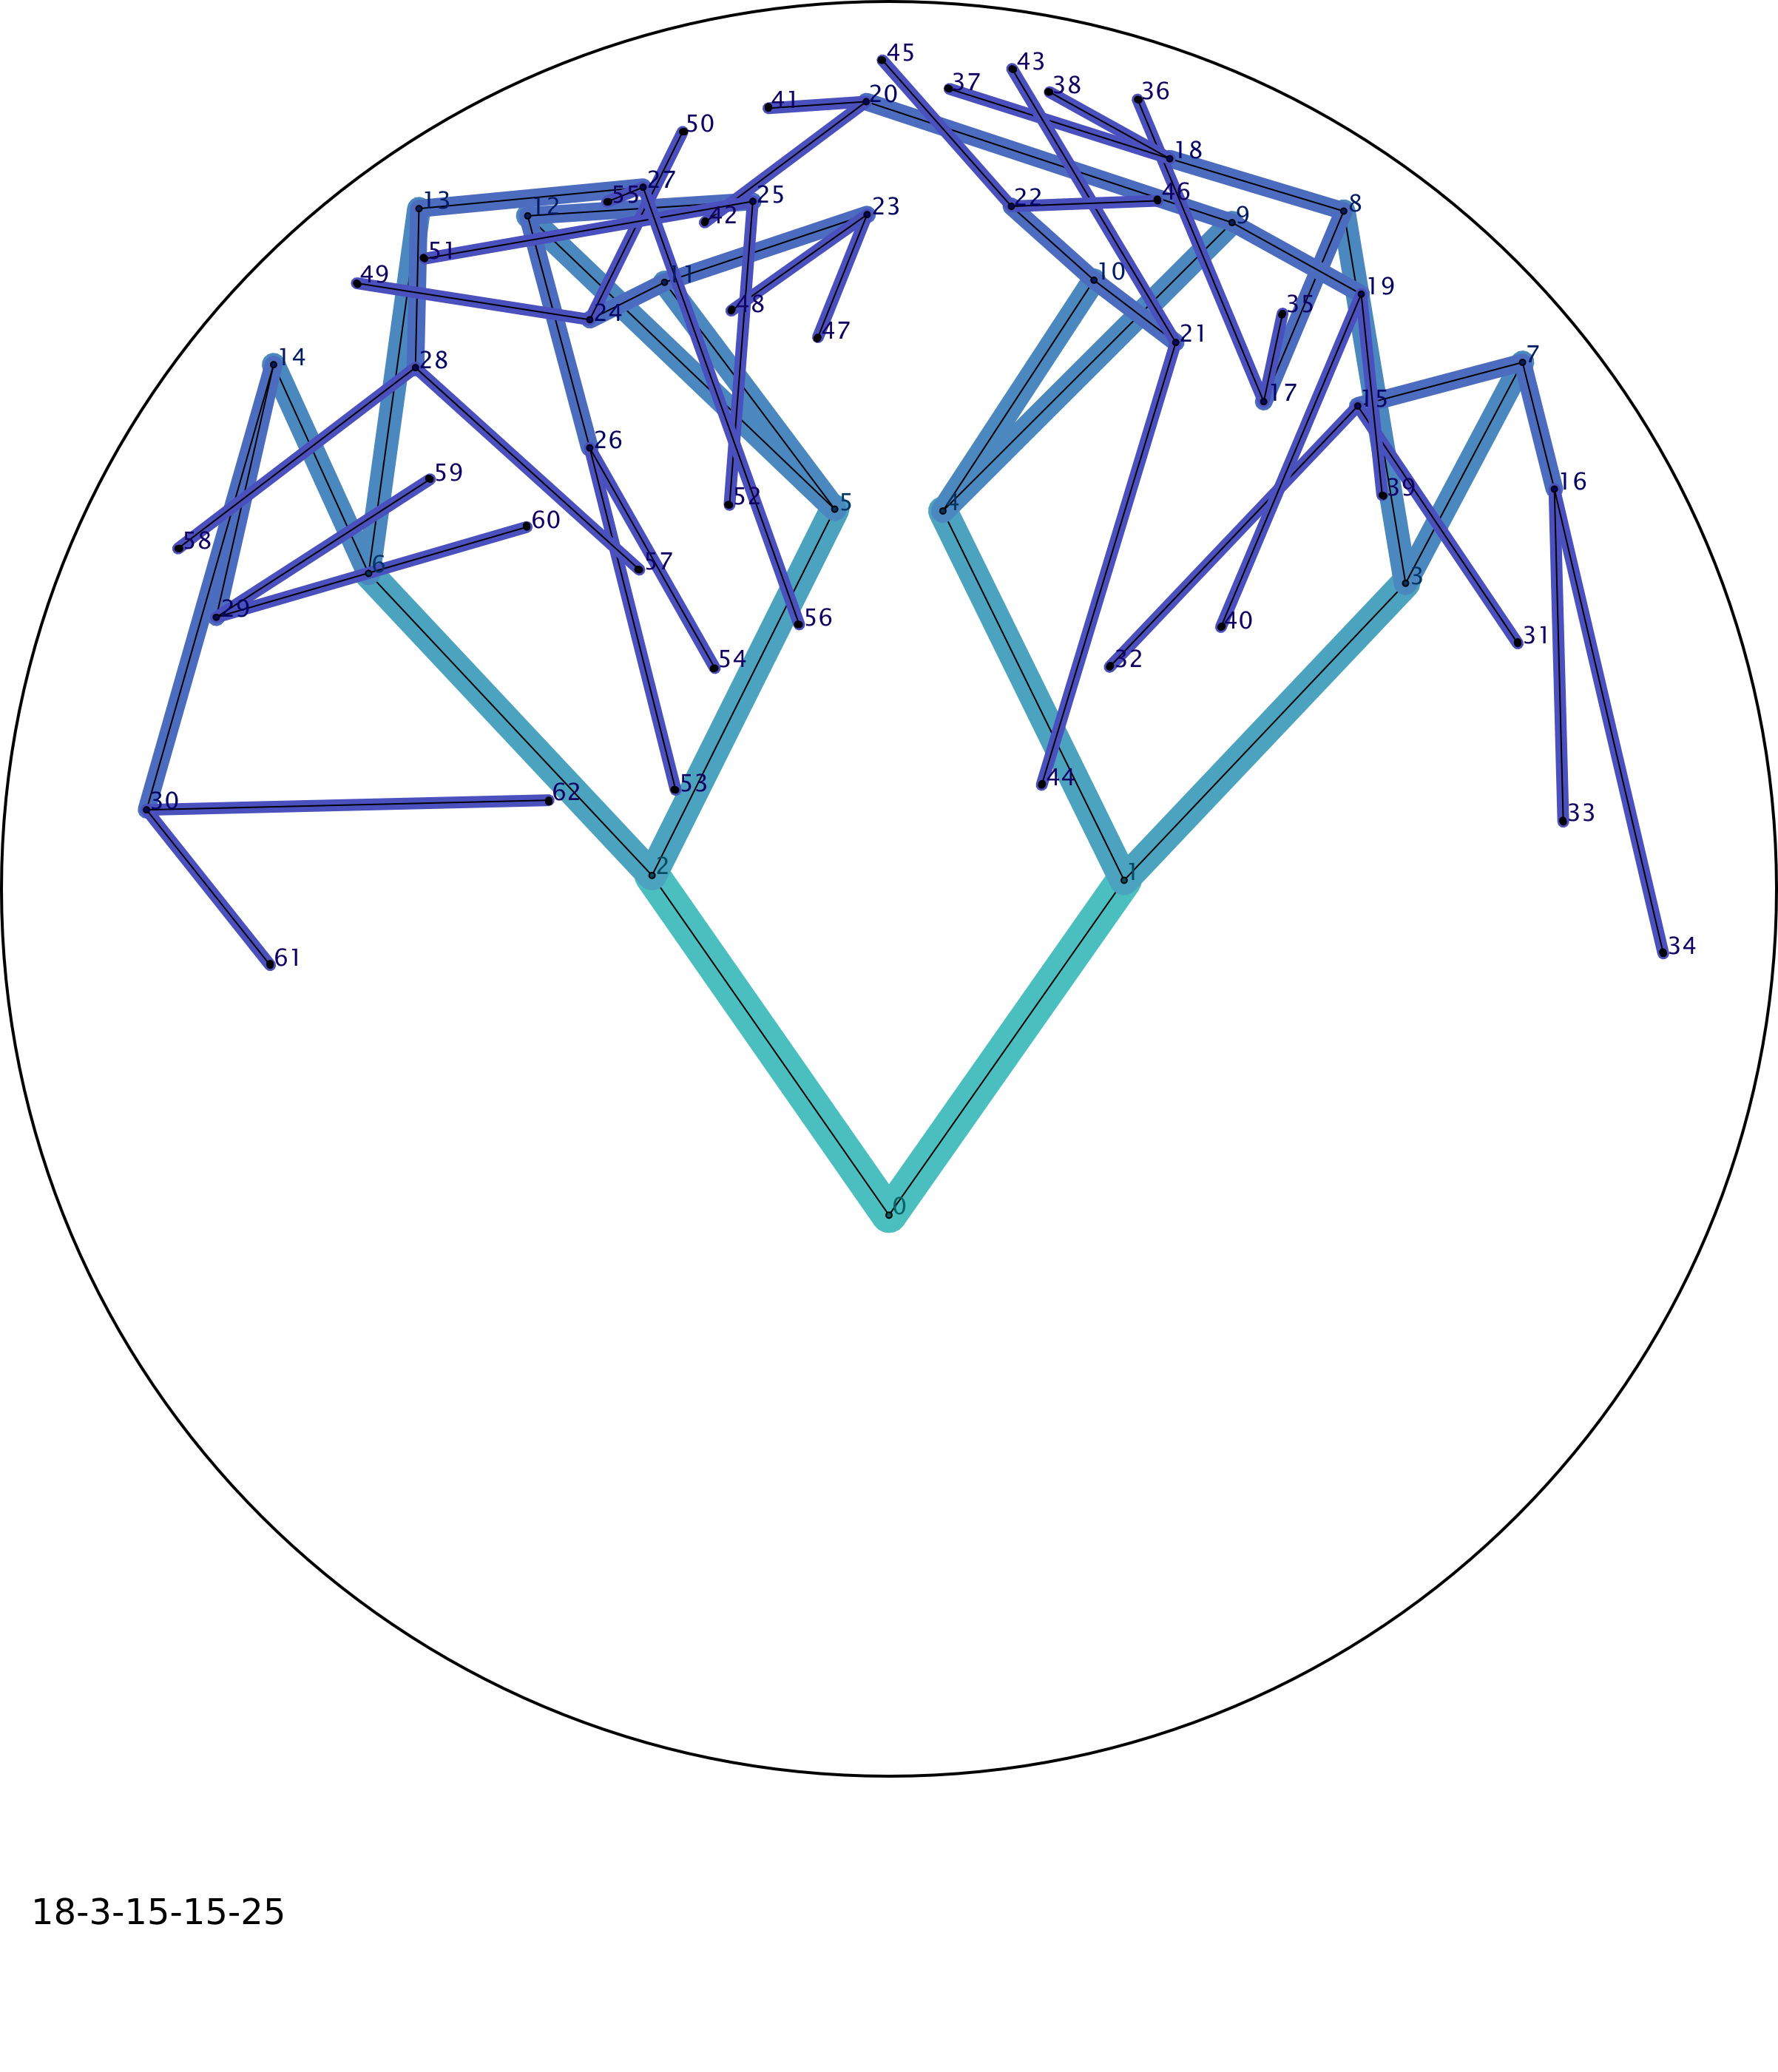
\includegraphics[width=\textwidth]{img_18-3-15-15-25}
\captionof{figure}{spawnAnglesDegree = +/-45}
\end{minipage}
\hspace{0.5cm}
\begin{minipage}[t]{\imgSize\textwidth}
\raisebox{0.175\totalheight}{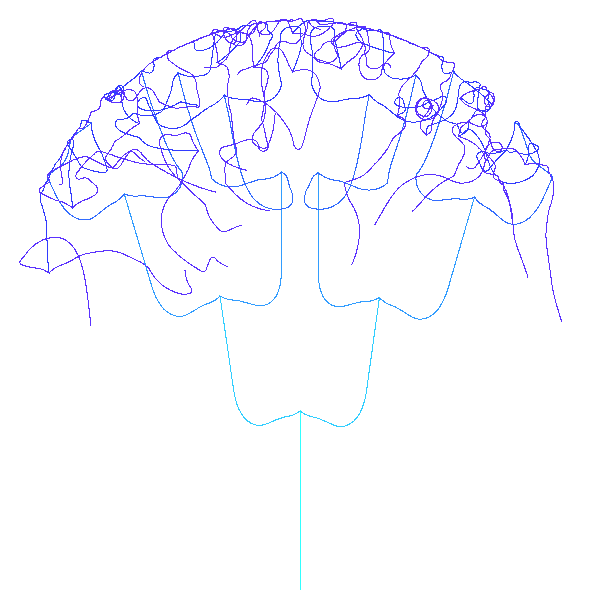
\includegraphics[width=\textwidth]{tank_spawnAnglesDegree_trace_18-3-15-15-25_1}}
\captionof{figure}{spawnAnglesDegree = +/-45}
\end{minipage}
\vspace{0.5cm}  

%90
\begin{minipage}[t]{\imgSize\textwidth}
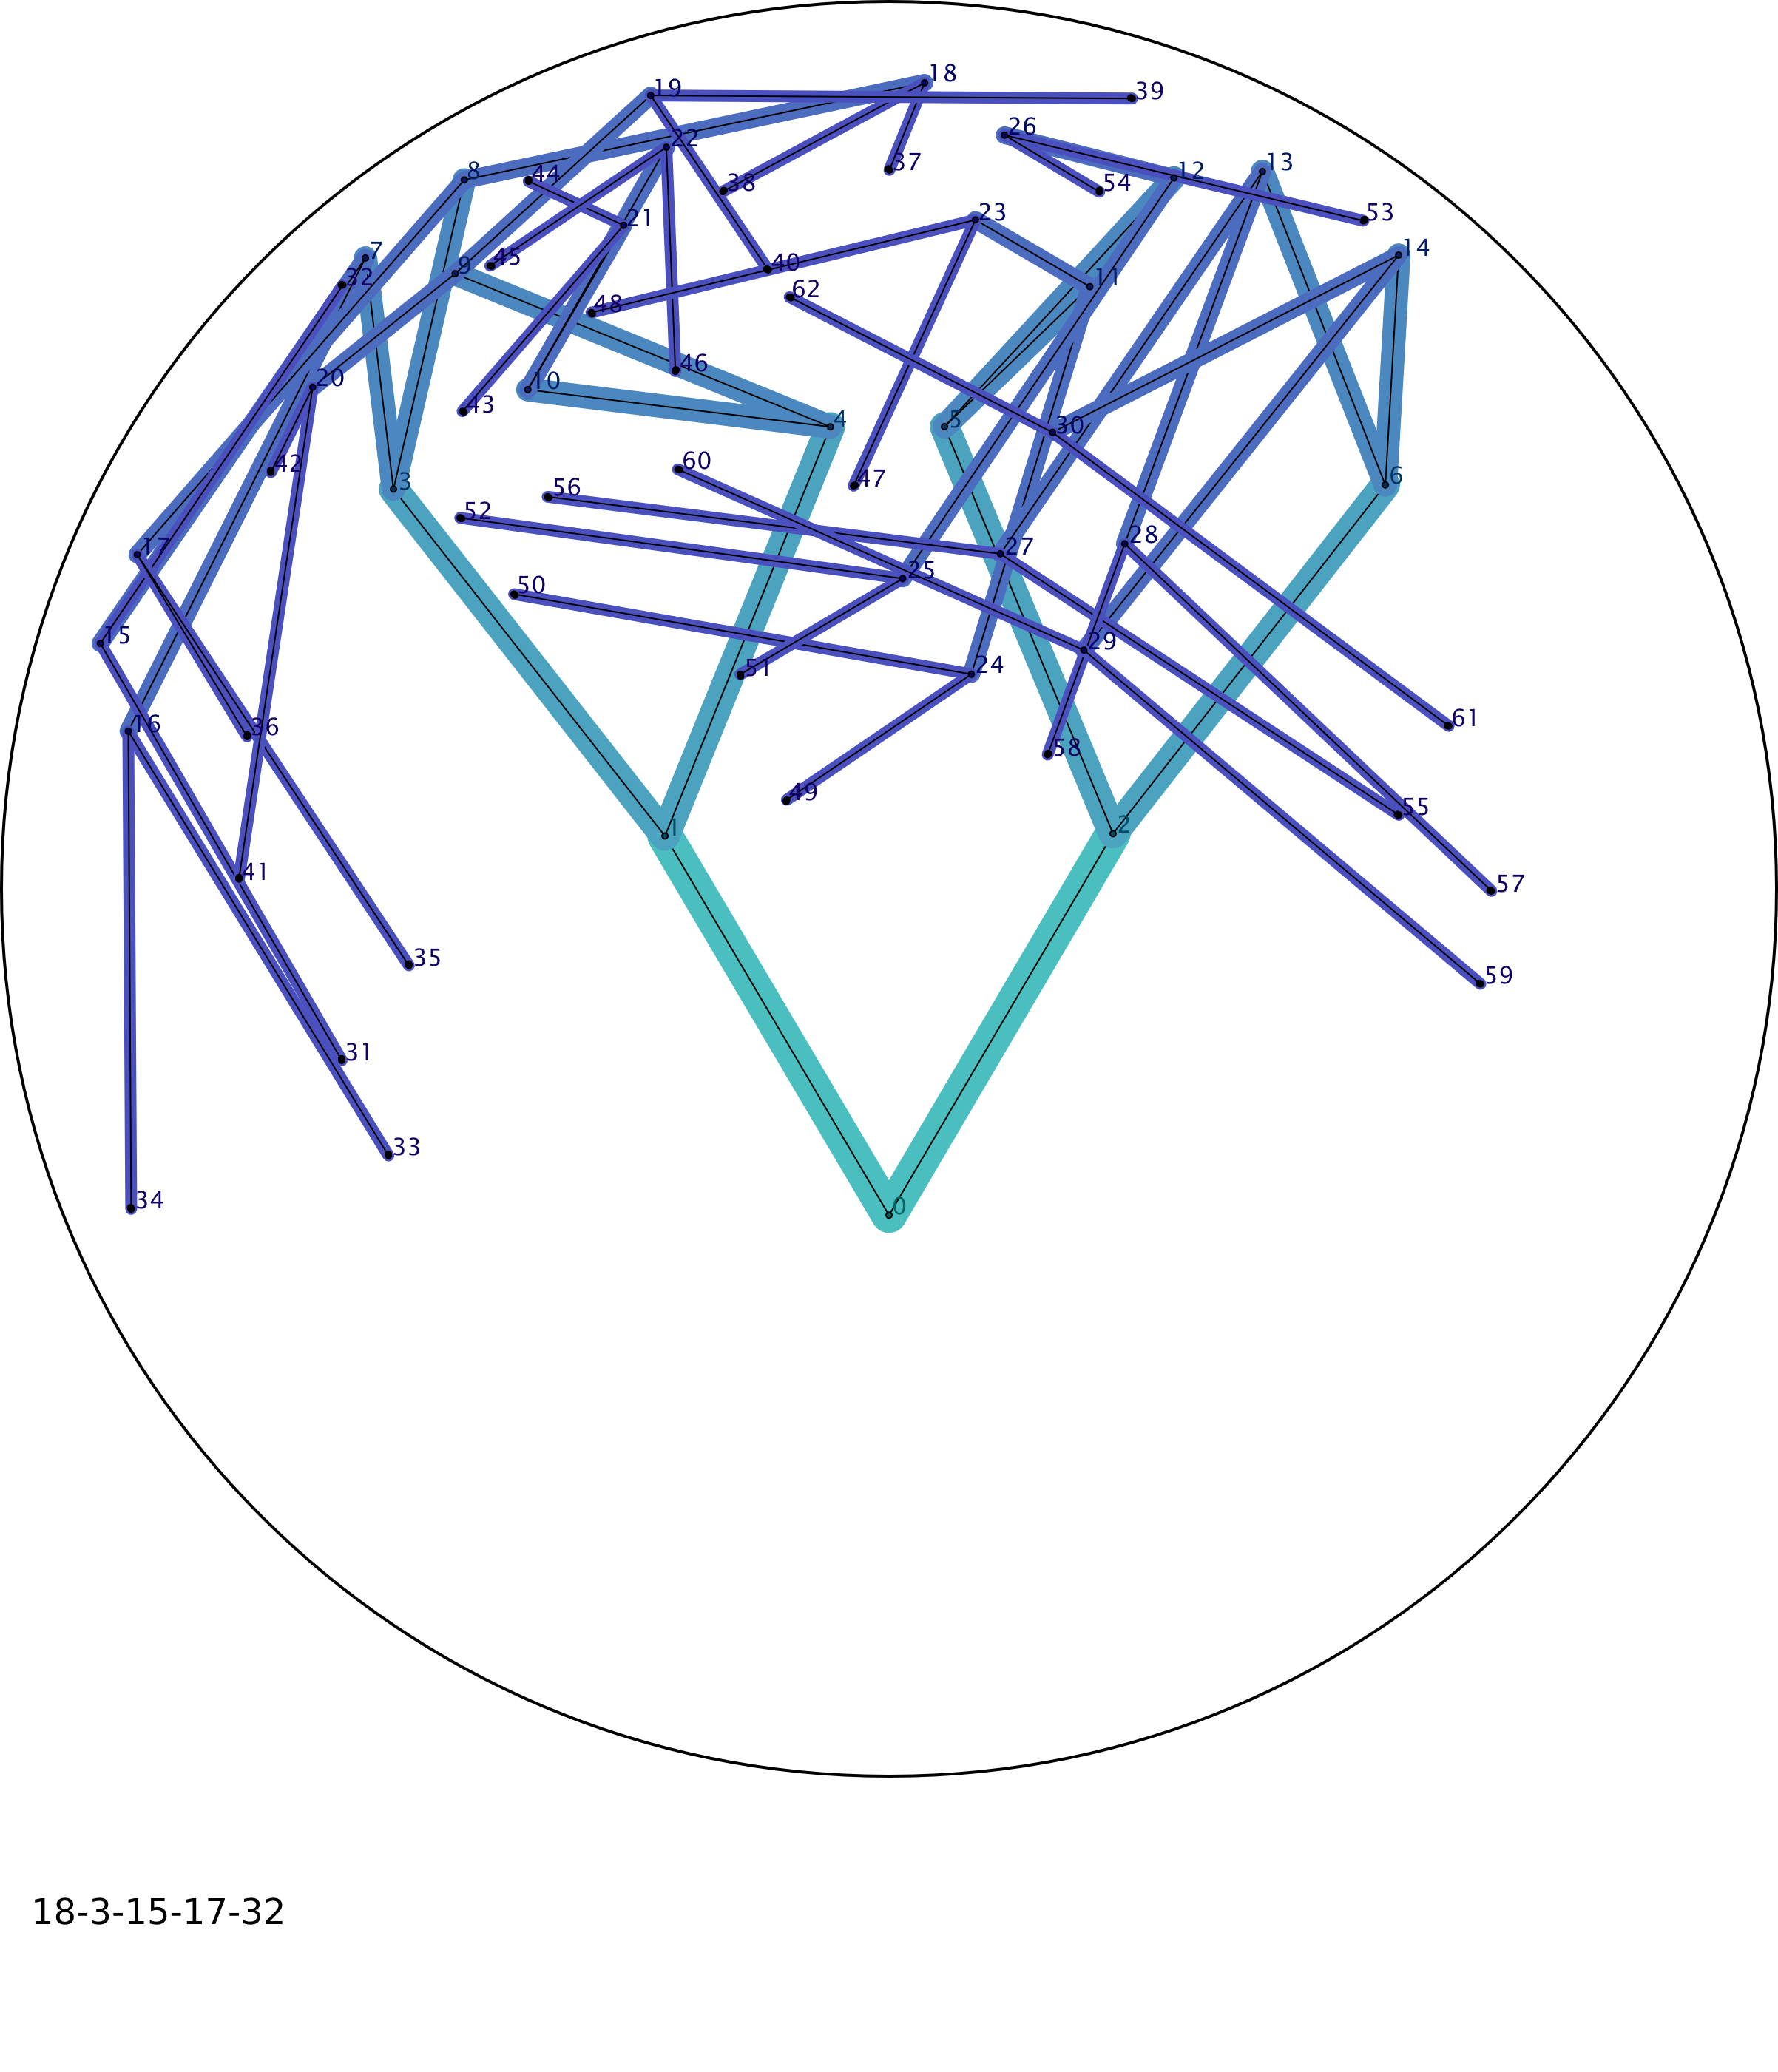
\includegraphics[width=\textwidth]{img_18-3-15-17-32}
\captionof{figure}{spawnAnglesDegree = +/-90}
\end{minipage}
\hspace{0.5cm}
\begin{minipage}[t]{\imgSize\textwidth}
\raisebox{0.175\totalheight}{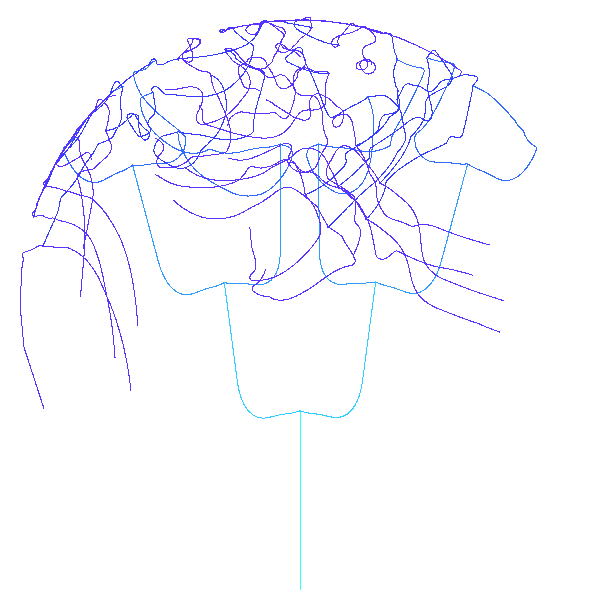
\includegraphics[width=\textwidth]{tank_spawnAnglesDegree_trace_18-3-15-17-32_1}}
\captionof{figure}{spawnAnglesDegree = +/-90}
\end{minipage}
\vspace{0.5cm} 

%135
\begin{minipage}[t]{\imgSize\textwidth}
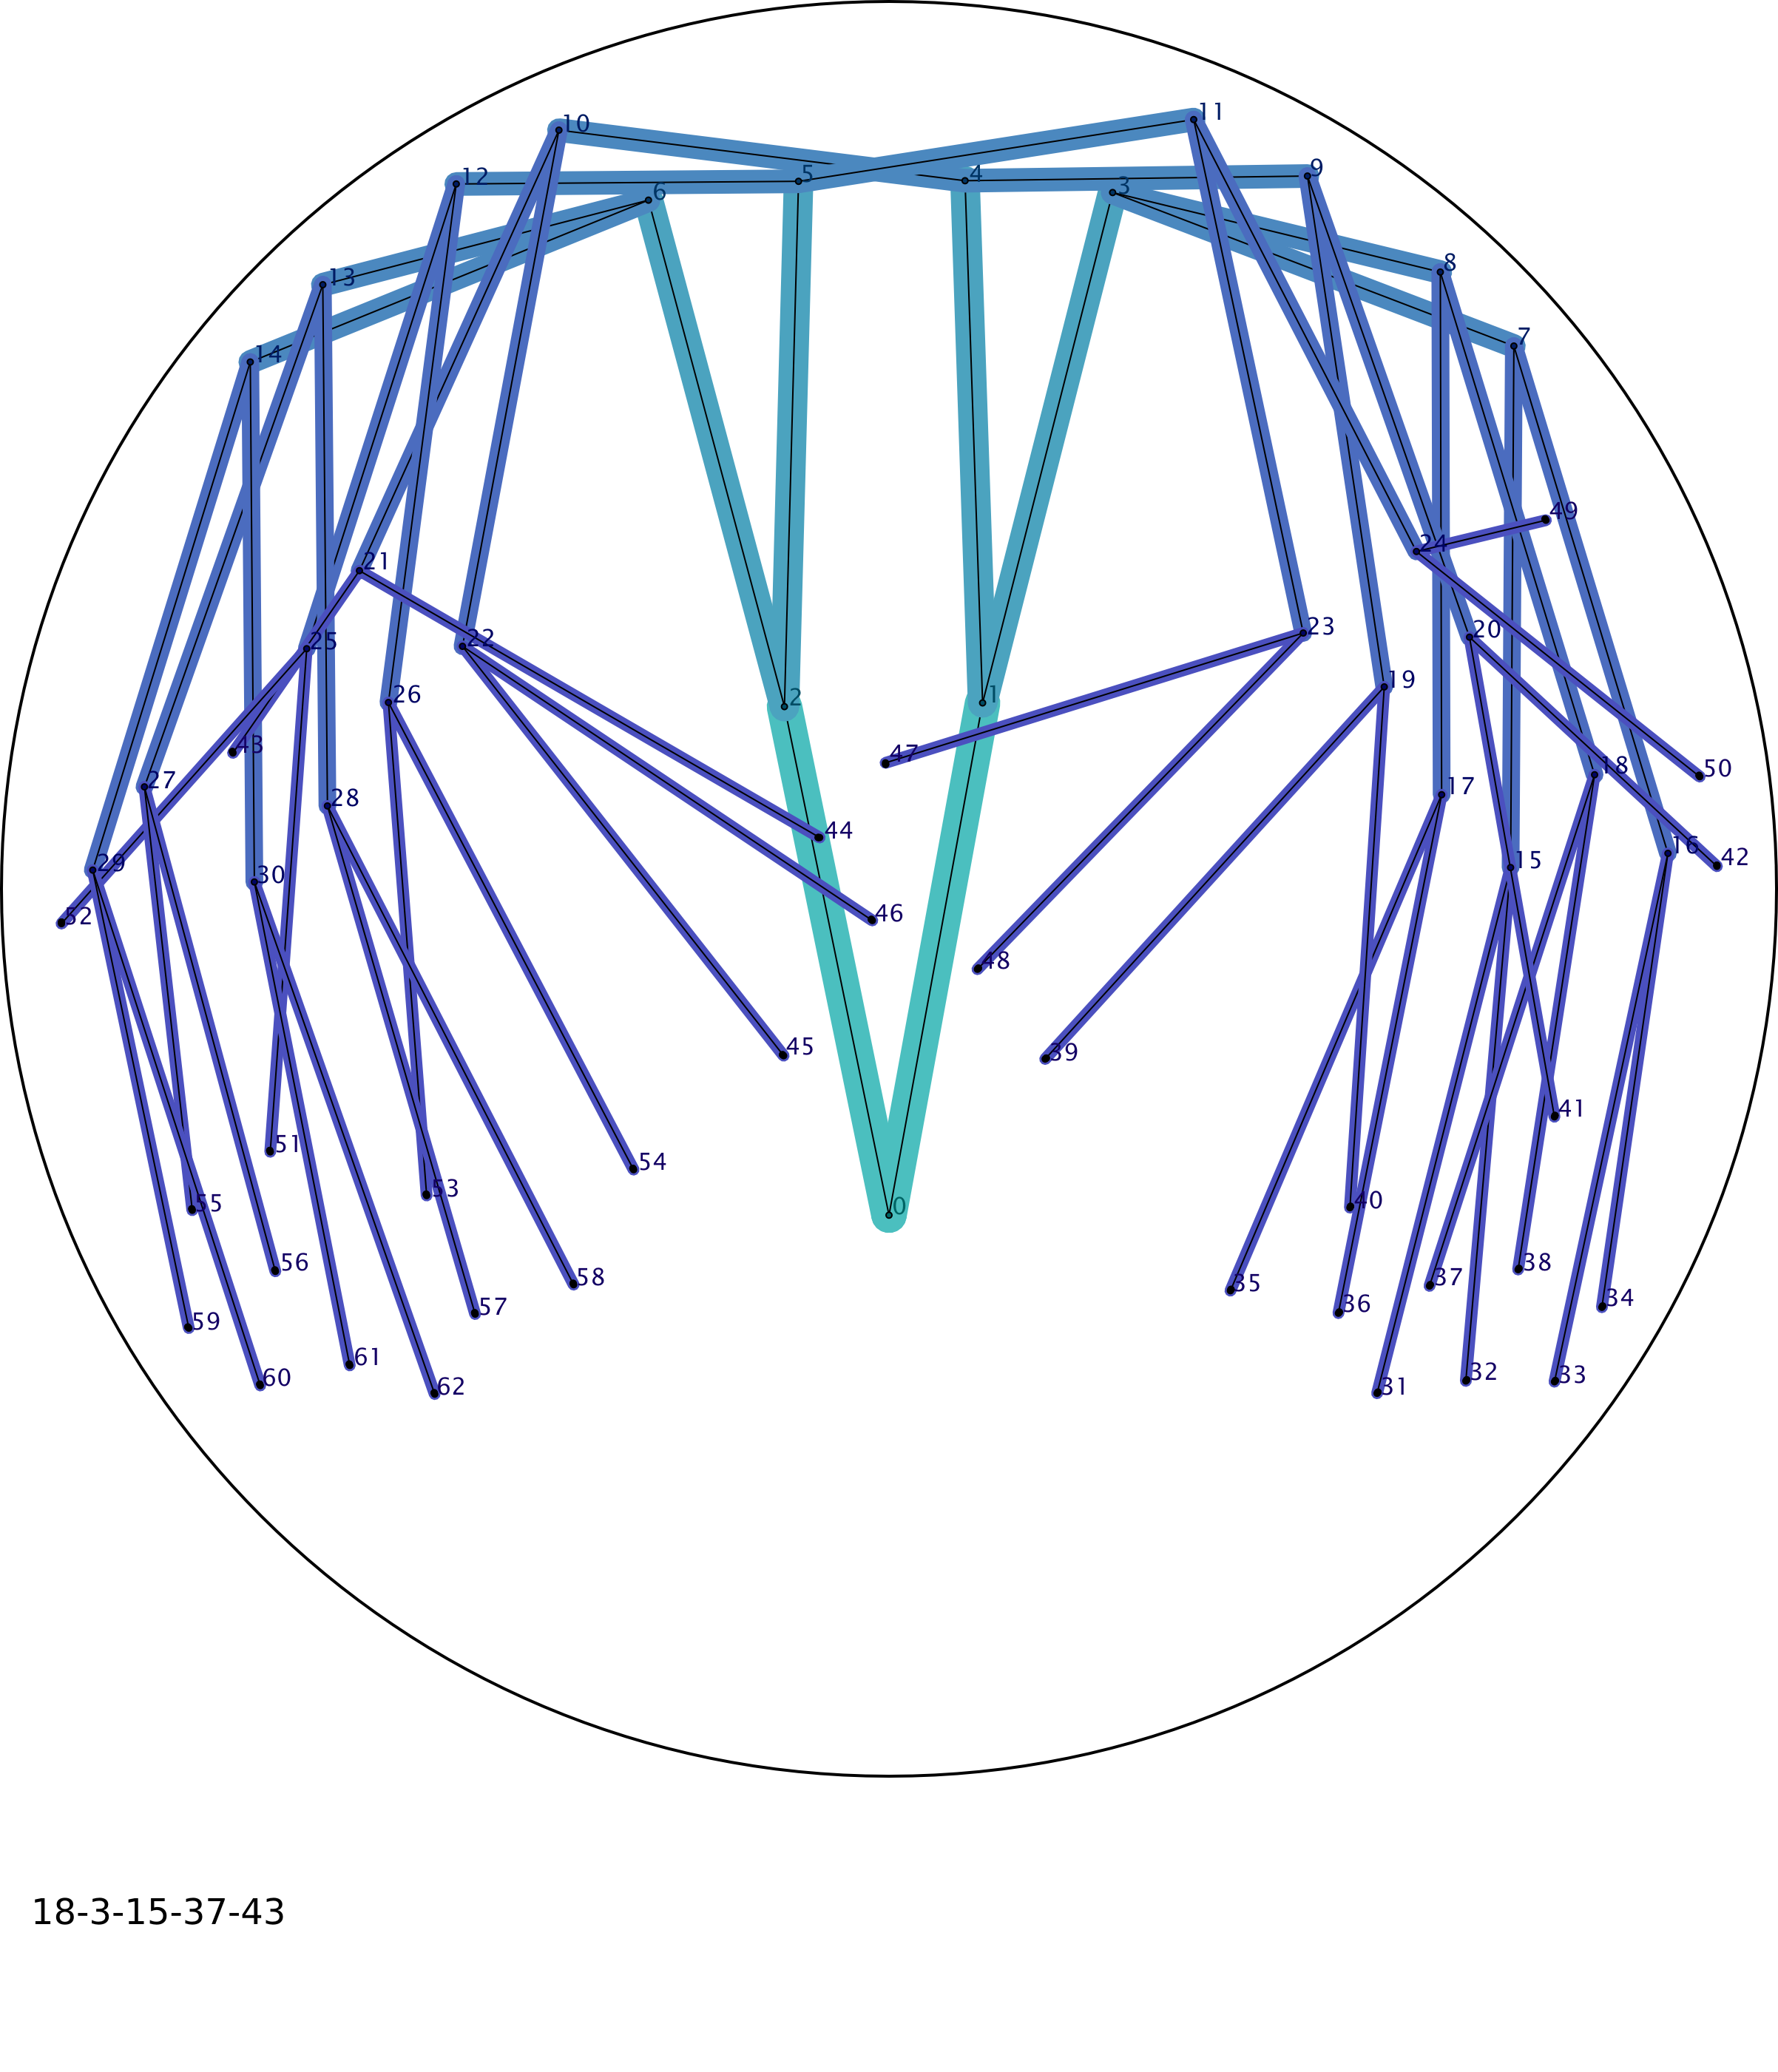
\includegraphics[width=\textwidth]{img_18-3-15-37-43}
\captionof{figure}{spawnAnglesDegree = +/-135 (default)}
\end{minipage}
\hspace{0.5cm}
\begin{minipage}[t]{\imgSize\textwidth}
\raisebox{0.175\totalheight}{\includegraphics[width=\textwidth]{tank_default_trace_18-3-15-37-43_1}}
\captionof{figure}{spawnAnglesDegree = +/-135 (default)}
\end{minipage}
\vspace{0.5cm}

%180
\begin{minipage}[t]{\imgSize\textwidth}
\includegraphics[width=\textwidth]{img_18-3-15-19-23}
\captionof{figure}{spawnAnglesDegree = +/-180}
\end{minipage}
\hspace{0.5cm}
\begin{minipage}[t]{\imgSize\textwidth}
\raisebox{0.175\totalheight}{\includegraphics[width=\textwidth]{tank_spawnAnglesDegree_trace_18-3-15-19-23_1}}
\captionof{figure}{spawnAnglesDegree = +/-180}
\end{minipage}
\vspace{0.5cm}

%--------------------------------------------------------------------
\section{Textile Implementation}
\subsection{Thoughts on Goals}

Throughout the whole development of the algorithms and parameter variations I played with several ideas on how to go from digital to textile. The basic idea was to use threads as entities or individuals. However, I was very indecisive about the details. Early ideas included just embroidering the movement of the fish or use the movements to (pseudo-) weave. I also came up with a Macramé-related knotting scheme, that resembled an RPG: each thread could win or lose in a fight against other threads. 

None of those concepts was interesting enough. All of them had a building or producing element in common, so I tried to turn that element upside down.
Working with textiles is usually constructing something, still there will be steps you have to reverse, because you made a mistake or the material was flawed. You have to untie the knot, unweave your cloth or just untangle the mess. Yet these unwanted destructive processes happen in favor of the final product.

I wanted to exaggerate the principle of destruction for my textile piece.
Still adhering to the threads as individuals it meant deconstructing the elements itself: one thread contains other, thinner threads.
The parent-child-relation between the fish in my tank fits in seamlessly with the construction-by-deconstruction-concept. The parent fish contains all the material needed to form the children, which then again contain everything for their children.

I will use a thread and split it up into subthreads, which match the connection between parent and children.


\subsection{Textile Piece I}
\subsubsection{Method and Tools}

\begin{minipage}[t]{0.48\textwidth}
    \raisebox{-0.9\totalheight}{\includegraphics[width=\textwidth]{stoffraster}}
    \captionof{figure}{Base material as canvas}
\end{minipage}
\hspace{0.5cm}
\begin{minipage}[t]{0.48\textwidth}
    For my first practical trial run I used evenweave with approximately 2mm per unit. To limit the size I scaled down the computed positions to fit a 100 by 100 grid (resulting in appr. 20cm by 20cm for the finished piece). The yellow thread was used as a counting help.
\end{minipage}
\vspace{0.5cm}
\begin{minipage}[t]{0.48\textwidth}
    \raisebox{-0.9\totalheight}{\includegraphics[width=\textwidth]{fadendetail}}
	\captionof{figure}{Applied material}
\end{minipage}
\hspace{0.5cm}
\begin{minipage}[t]{0.48\textwidth}
	Because my generations of fish are based on the number 2, I also need thread based on number 2. So I used cotton wool threads each already containing 8 ($=2^3$) sub-threads when feazed.\\
	To be able to manage the threads and associate them with one fish id I simply attached some paper to the string groups. The positions are directly read from the text in the log file.
\end{minipage}
\vspace{0.5cm}

\begin{minipage}[t]{\textwidth}
\scriptsize
\begin{verbatim}
tank cx,cy,radius: 300.0 300.0 300.0
starter fish: 1
start dir: 1.0 1.0
start pos: 300.0, 300.0
wall/neighbor 0.9/0.1
maxGenerations 7
maxChildren 2

spawnTime 5000ms
spawnAnglesDegree 135.0 -135.0
turnSpeed 0.0051/ms
private radius / company radius 40.0 / 75.0

fish:
0 g:0 born 300.0 300.0 : 140 140 c: 
0 g:0 died 409.58185 409.58185 : 191 191 c: 1 2 
1 g:1 died 434.7048 547.7104 : 203 256 c: 3 4 
2 g:1 died 547.1275 435.0458 : 255 203 c: 5 6 
3 g:2 died 299.06696 479.5542 : 140 224 c: 7 8 
4 g:2 died 290.70502 579.7467 : 136 271 c: 9 10 
5 g:2 died 578.5094 290.45987 : 270 136 c: 11 12 
6 g:2 died 474.91296 301.06262 : 222 140 c: 13 14
...
\end{verbatim}
\captionof{figure}{First part of the used log file}
\end{minipage}
\vspace{0.5cm}

\begin{minipage}[t]{0.46\textwidth}
\includegraphics[width=\textwidth]{img_17-3-10-2-8}
\captionof{figure}{Connection lines between (dead) fish of 7 generations}
\end{minipage}
\hspace{0.5cm}
\begin{minipage}[t]{0.46\textwidth}
\includegraphics[width=\textwidth]{tankA_trace_17-3-10-2-8_1}
\captionof{figure}{Traces of the movement of the fish while living}
\end{minipage}
\vspace{0.5cm}
\begin{minipage}[t]{\textwidth}
    \includegraphics[width=\textwidth]{frontback}
	\captionof{figure}{Total view of the experiment and details on the back. For 7 generations of fish, each having 2 children I need $2^7$ threads (128). Using the $2^3$ cotton strings, I need 16 strings in total - which is quite thick. I tried to fit it through one "grid point" - even when I succeeded the accuracy of the grid was physically compromised, so I decided to dilute the positions for the first maybe also for the second generation of fish. The starting point for the fish is 50/50. After dividing the thick 16-strings-cord into 4 subcords with 4 strings each, the starting points are 51/50, 49/50, 50/49, 50/51.}
	\label{trial1}
\end{minipage}
\vspace{0.5cm}

\subsubsection{Outcome and Conclusion}
The left of Fig.\ref{trial1} shows the state of the first experiment when I decided I was not getting anywhere near to what I wanted. One reason was a simple mistake when determining the thread count: For 7 generations I actually would only have needed $2^6$ instead of $2^7$ single threads in the end, because I forgot to start counting at $2^0$. This would have reduced the thickness of the starting thread by half and also changed the appearance significantly.\\
A more serious problem for me was that the visual outcome was somehow off. Maybe I chose the evenweave's units too large or the wrong color, but most importantly the intermediate result did not have the properties I expected it to have: it was neither 2D nor 3D, neither did I get the threads to be stiff and straight enough for the connections of the fish nor did they show the actual movement of a fish during its life cycle.
This first piece was an unsatisfying accumulation of imprecise craftsmanship, so I thought about other possibilities to work with the pattern in the material world.

\subsection{Textile Piece II}
\subsubsection{Method and Tools}
Unlike techniques such as stitching or weaving were the interaction between up and down movements is crucial, the destruction concept I want to explore is independent from that. That means I need a more robust canvas. I decided to use a non-textile base, namely a semi-see-through PVC sheet. Although I thought about cutting holes in the PVC to guide the threads, as said before, this would artificially add something to the concept that does not belong to it. Instead, a hot glue gun was used to fixate the splitting points and keep the strings neatly in place.
Pieces of a series can be stacked and the viewer can easily compare the different layouts of the strings.

- same cotton wool, but only 6 generations, meaning $2^5 = 32$ sub-threads which equals 4 of the normal threads. Hand-dyed to achieve a color gradient from dark blue to green to yellow to white. The gradient helps the viewer to distinguish the generations.

\subsubsection{Outcome and Conclusion}
- glue points add a subtle touch.

\section{Summary}

%what did I discover/explore?


%----------------------------------------------------------------------------------------------------

%====================================================================================================
\newpage
\section*{Code?}

%put the code here:
%\begin{lstlisting}
%\end{lstlisting}

%\bibliographystyle{plain}
%\bibliography{references}
\end{document}

